\documentclass[12pt,a4paper]{article}

%%%%%%%%% Preamble
\usepackage[paperheight=29.7cm, paperwidth=21cm,nomarginpar,textwidth=19cm,headheight=2.5cm,top=1.5cm,bottom=1.5cm]{geometry}
% used for figures:
\usepackage{graphicx}
% math fonts etc.:
\usepackage{amsmath,amsfonts,amsthm,latexsym,amssymb}
\usepackage{pdfpages}
\usepackage{caption,subcaption}
\usepackage{hyperref}
\hypersetup{
	colorlinks,
	citecolor=black,
	filecolor=black,
	linkcolor=blue,
	urlcolor=black
}
\usepackage{wrapfig}
\setlength\intextsep{2pt} % avoid too much space around figure (can be set to 0pt at maximum)

\graphicspath{ {figures/} }
%%%%%%%%%%

\begin{document}
	\tableofcontents
	\listoffigures
	\newpage
	\begin{center}
		\textcolor{orange}{\Large {\bf{Car accidents case study}}}
	\end{center}
	
	\section{Business context}
Car crashes are a leading cause of injury and death worldwide, making the improvement of vehicle safety a critical concern for car manufacturers. With advancements in technology and engineering, manufacturers are continuously seeking ways to design safer vehicles to reduce fatalities and severe injuries in the event of a crash. Despite these efforts, understanding the precise factors that contribute to survival in car crashes remains a complex challenge.

The problem arises from the nature of car accidents, where various elements such as impact speed, the use of safety features, the type of collision, and the demographics of the occupants all play significant roles. Each crash is unique, and even minor variations can significantly affect the outcome for the occupants. This complexity necessitates a detailed analysis to identify which factors are most influential in determining survival outcomes. Solving the problem of car crash survival is essential for several reasons:
\begin{itemize}
	\item Safety Regulations: Enhanced understanding of crash dynamics informs the development of stricter safety regulations and standards, ensuring that all vehicles on the road meet minimum safety requirements.
	\item Design Improvements: Insights from crash data drive innovations in vehicle design, leading to the creation of safer cars that better protect occupants during accidents.
	\item Public Health: Reducing fatalities and severe injuries from car crashes has a significant impact on public health, decreasing the burden on healthcare systems and improving overall community well-being.
	\item Consumer Confidence: As manufacturers improve vehicle safety, consumer confidence in the automotive industry increases. Buyers are more likely to invest in vehicles that are proven to offer better protection in the event of a crash.
\end{itemize}
Over the last year, the Department of Road Transport has witnessed a 15\% year-over-year rise in the number of car crashes happening in urban areas. While they have identified the causes of these accidents post-facto, their goal is to preempt the risk and increase road safety.

We have been hired as data scientists and provided with a sample of historical car crash data spanning five years. This dataset includes various attributes of the cars and the occupants relevant to the crashes. Our objective is to analyze this data, identify patterns in car crashes, and build a predictive model to determine the likelihood of survival in car crashes based on these factors. Additionally, we aim to identify the most critical factors that influence survival outcomes. This analysis will help the department develop necessary safety regulations that must be adopted by all vehicle manufacturers and users.
	
	\section{Exploratory data analysis}
	\subsection{Data set description}
	\begin{figure}[h]
		\centering
		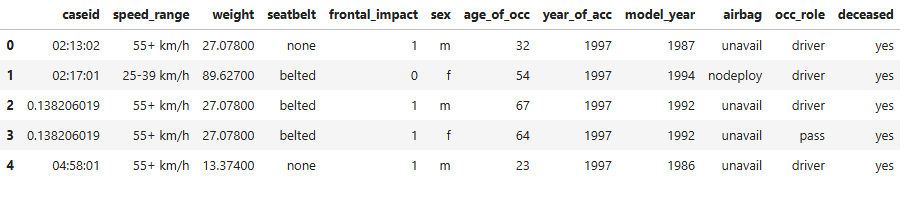
\includegraphics[width=0.85\textwidth]{dataset.png}
		\caption{A snapshot of data set used for analysis.}
		\label{fig:dataset}
	\end{figure}
The dataset provided gives detailed information on automobile accidents, with each row representing a different case. Here are the key points:

Accident Details: Includes speed range, vehicle weight, and whether the impact was frontal.
Driver Information: Records the sex and age of the driver, as well as seatbelt usage.
Vehicle Information: Contains the year of the accident and the model year of the vehicle.
Outcome: Indicates if an airbag was deployed and whether the occupant was released from the hospital or deceased.

The description of each field is as follows : 
caseid: A unique identifier for each accident case.
speed\_range: The speed range of the vehicle at the time of the accident (e.g., 55+ km/h, 25-39 km/h).
weight: The weight of the vehicle involved in the accident.
seatbelt: Indicates whether the occupant was using a seatbelt (e.g., belted, none).
frontal\_impact: A binary indicator showing if the impact was frontal (1 for yes, 0 for no).
sex\_of\_driver: The gender of the driver (e.g., m for male, f for female).
age\_of\_occ: The age of the occupant at the time of the accident.
year\_of\_acc: The year when the accident occurred.
model\_year: The model year of the vehicle involved in the accident.
airbag: Indicates whether the airbag was deployed (e.g., deploy, nodeploy).
occ\_role: The role of the occupant in the vehicle (e.g., driver, passenger).
deceased: Indicates whether the occupant was deceased as a result of the accident (yes or no). There are total 11,217 records in our dataset. We did not find any irregularities or missing values in the data set, therefore we will move to analysis with out much description of data cleaning and treatment. We created one derived column veh\_usage\_duration to indicate how much time the vehicle had been used before the accident.	
	\begin{figure}[h]
		\centering
		\begin{subfigure}[t]{0.24\textwidth}
			\centering
			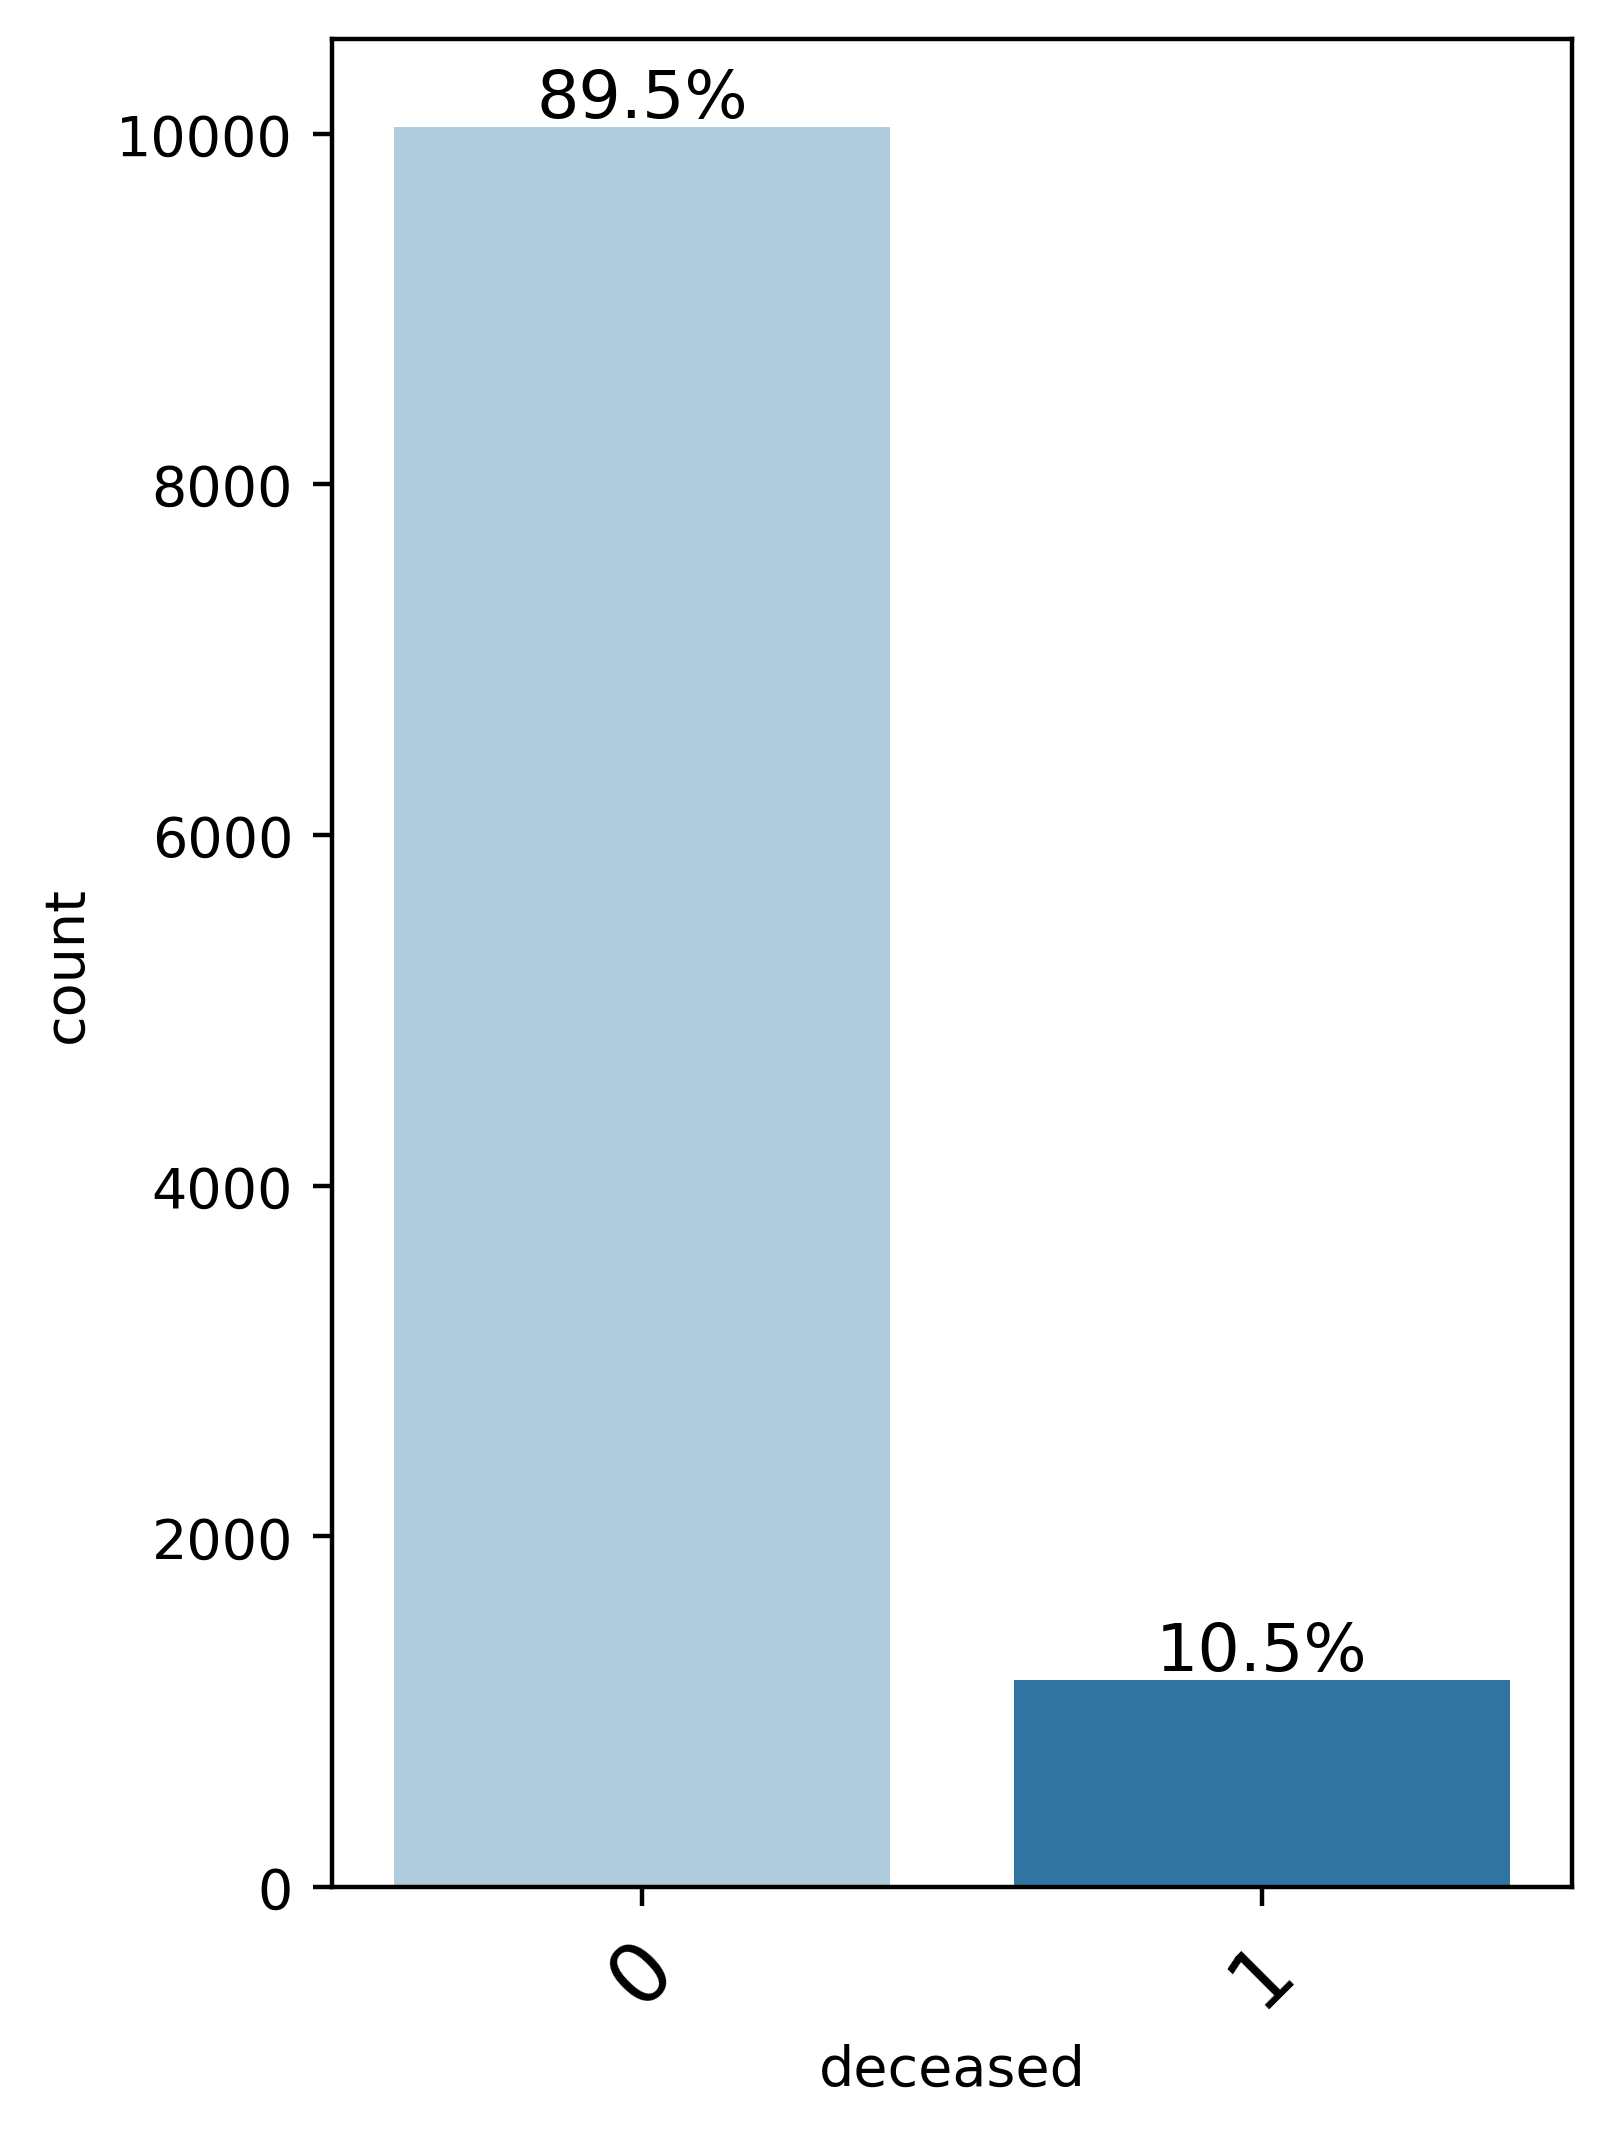
\includegraphics[width=4cm]{deceased_dist.png}
			\caption{}
			\label{fig:deceased_dist}
		\end{subfigure}
		\hfill
		\begin{subfigure}[t]{0.24\textwidth}
			\centering
			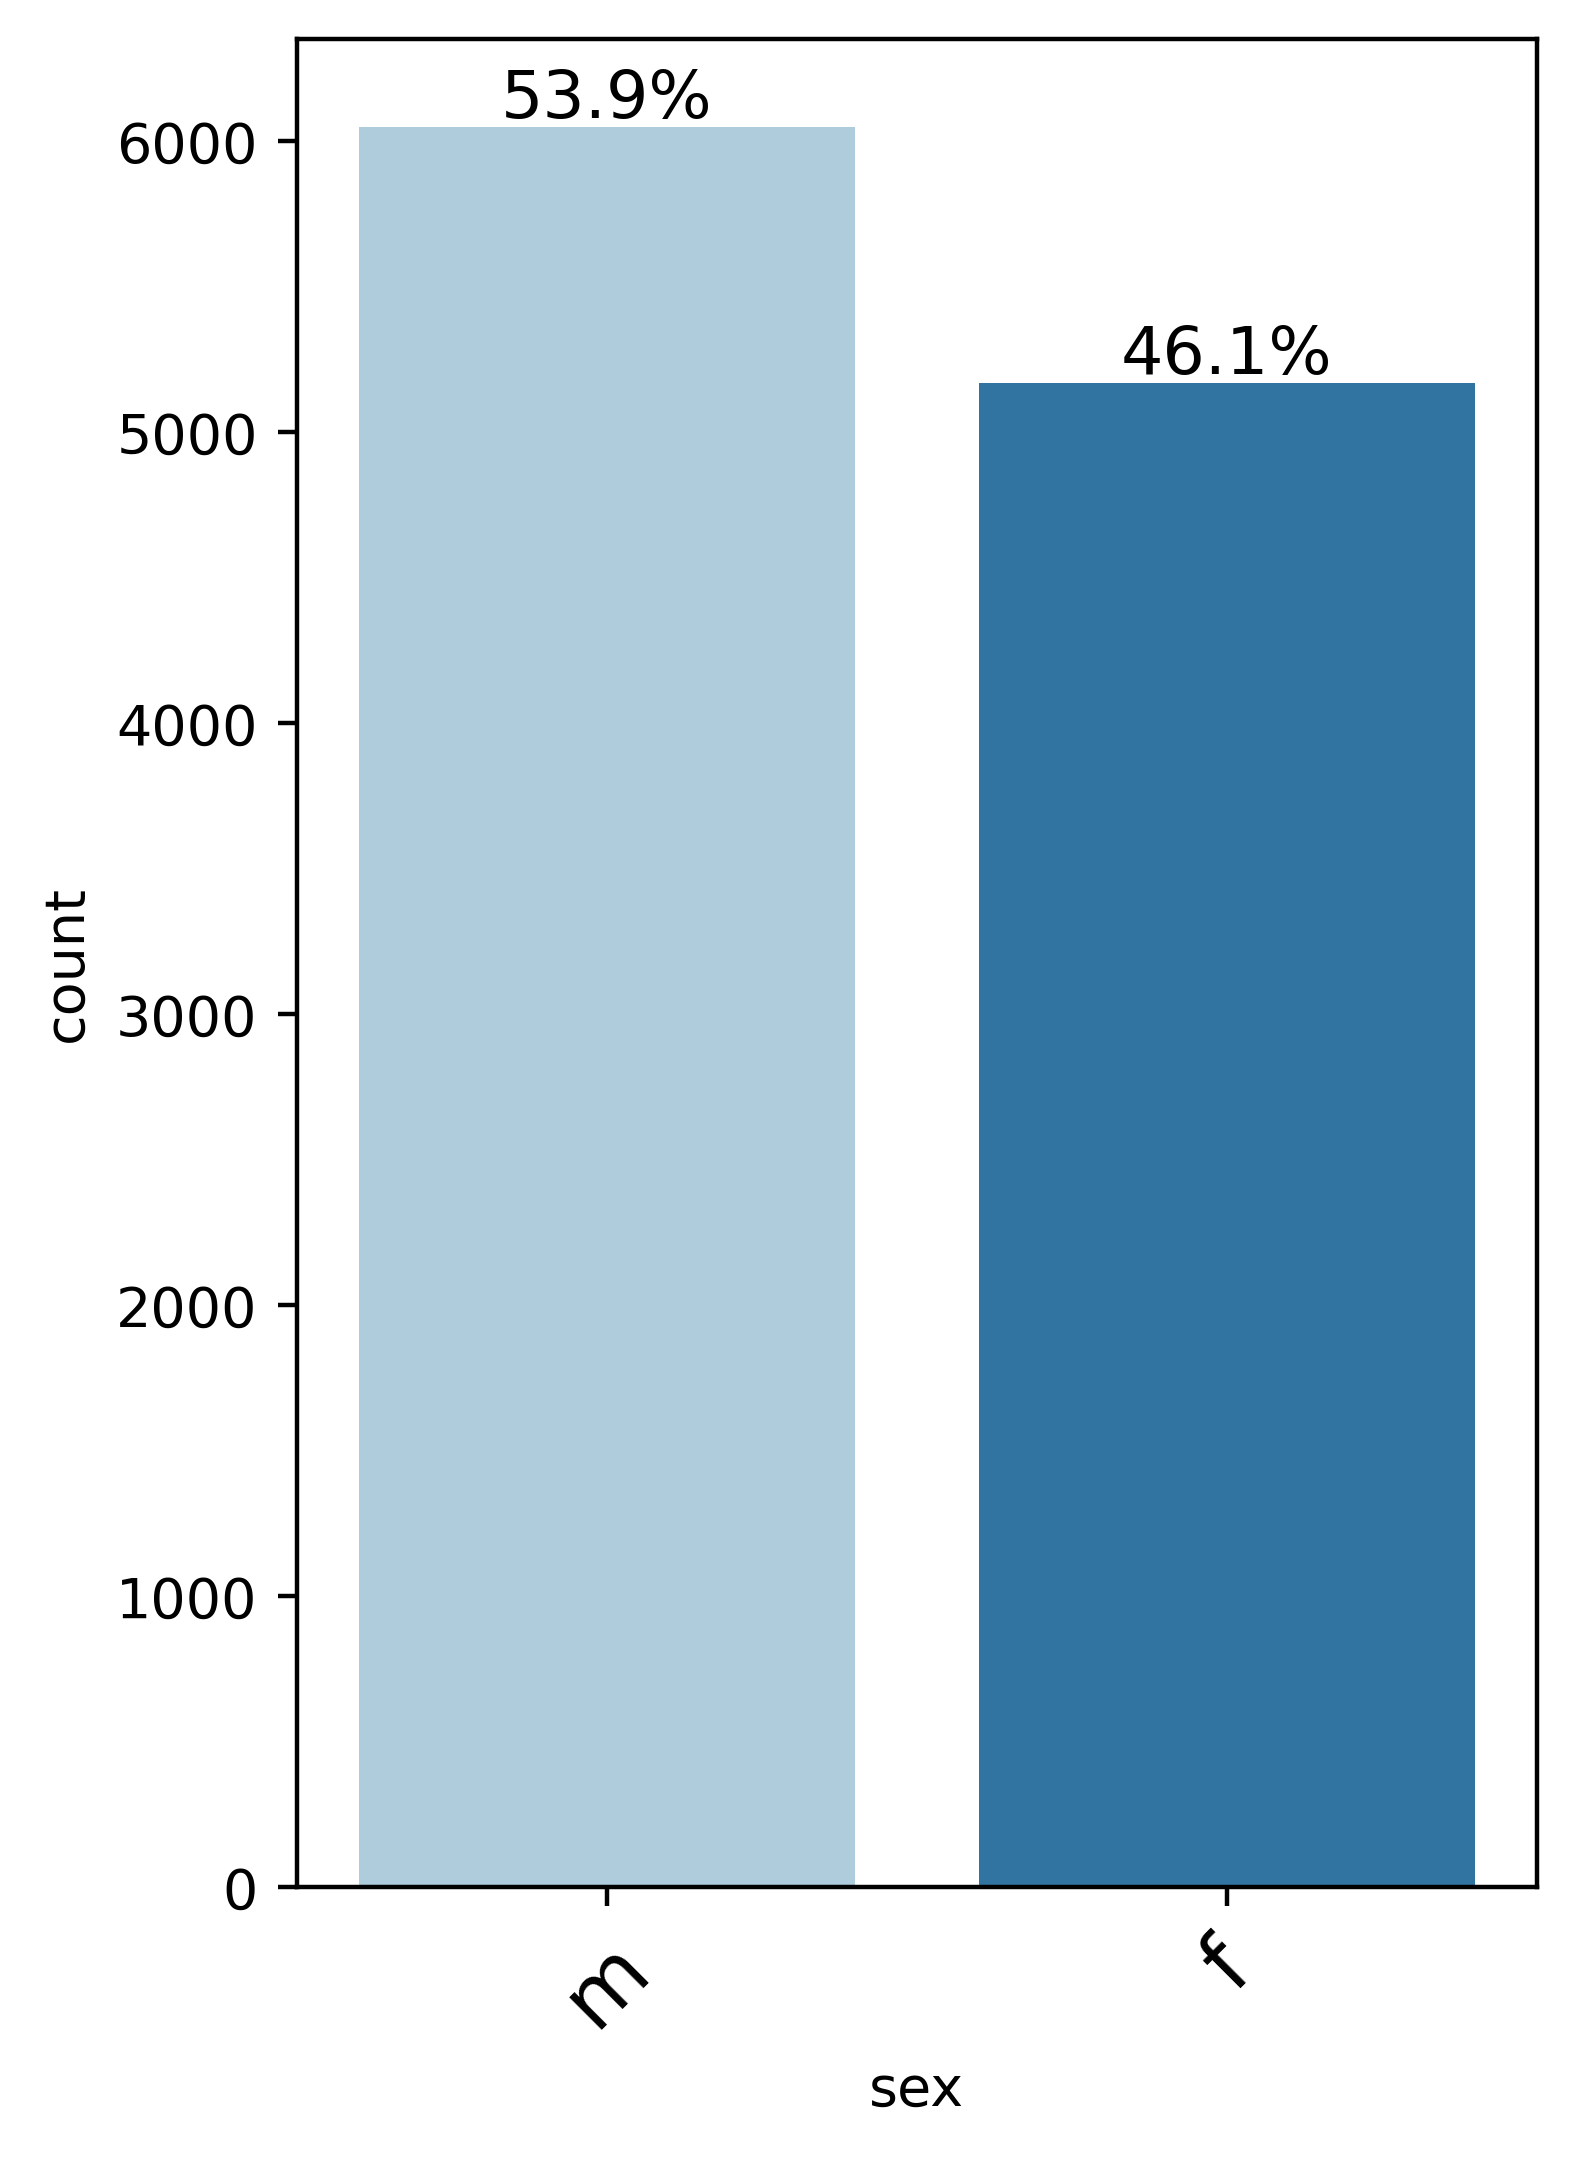
\includegraphics[width=4cm]{sex_dist.png}
			\caption{}
			\label{fig:sex_dist}
		\end{subfigure}
		\hfill
		\begin{subfigure}[t]{0.24\textwidth}
			\centering
			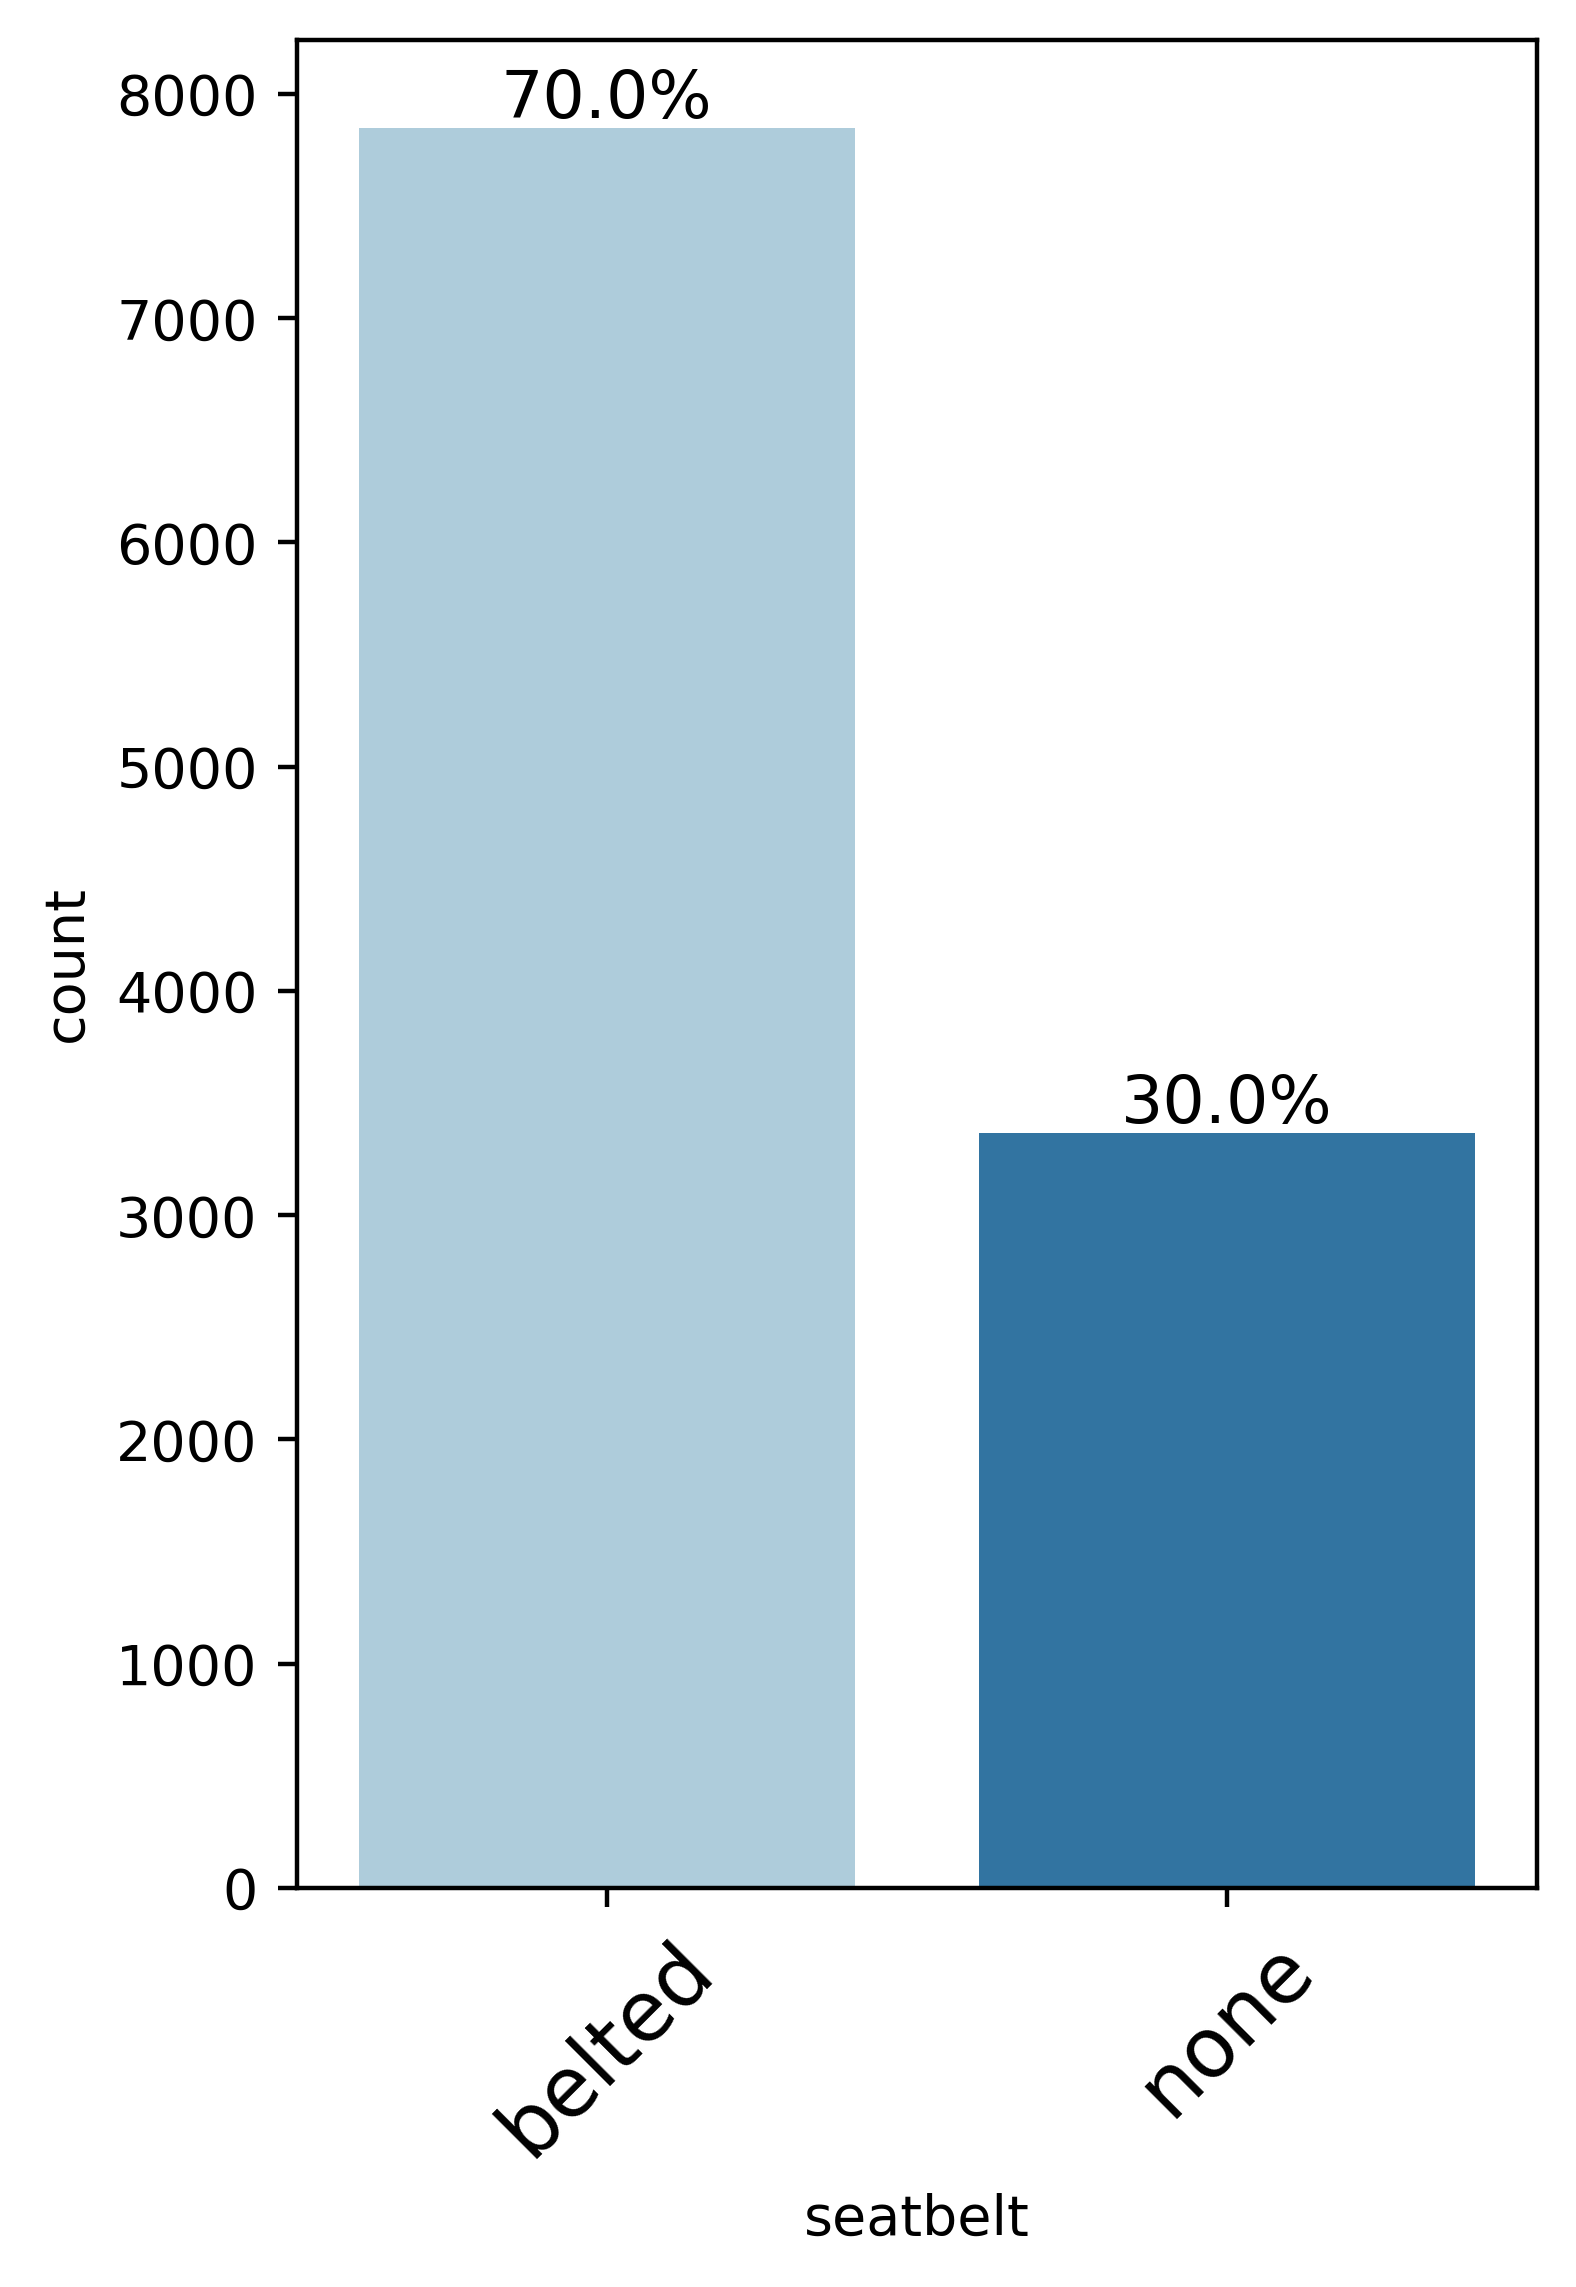
\includegraphics[width=4cm]{seatbelt_dist.png}
			\caption{}
			\label{fig:seatbelt_dist}
		\end{subfigure}
		\hfill
		\begin{subfigure}[t]{0.24\textwidth}
			\centering
			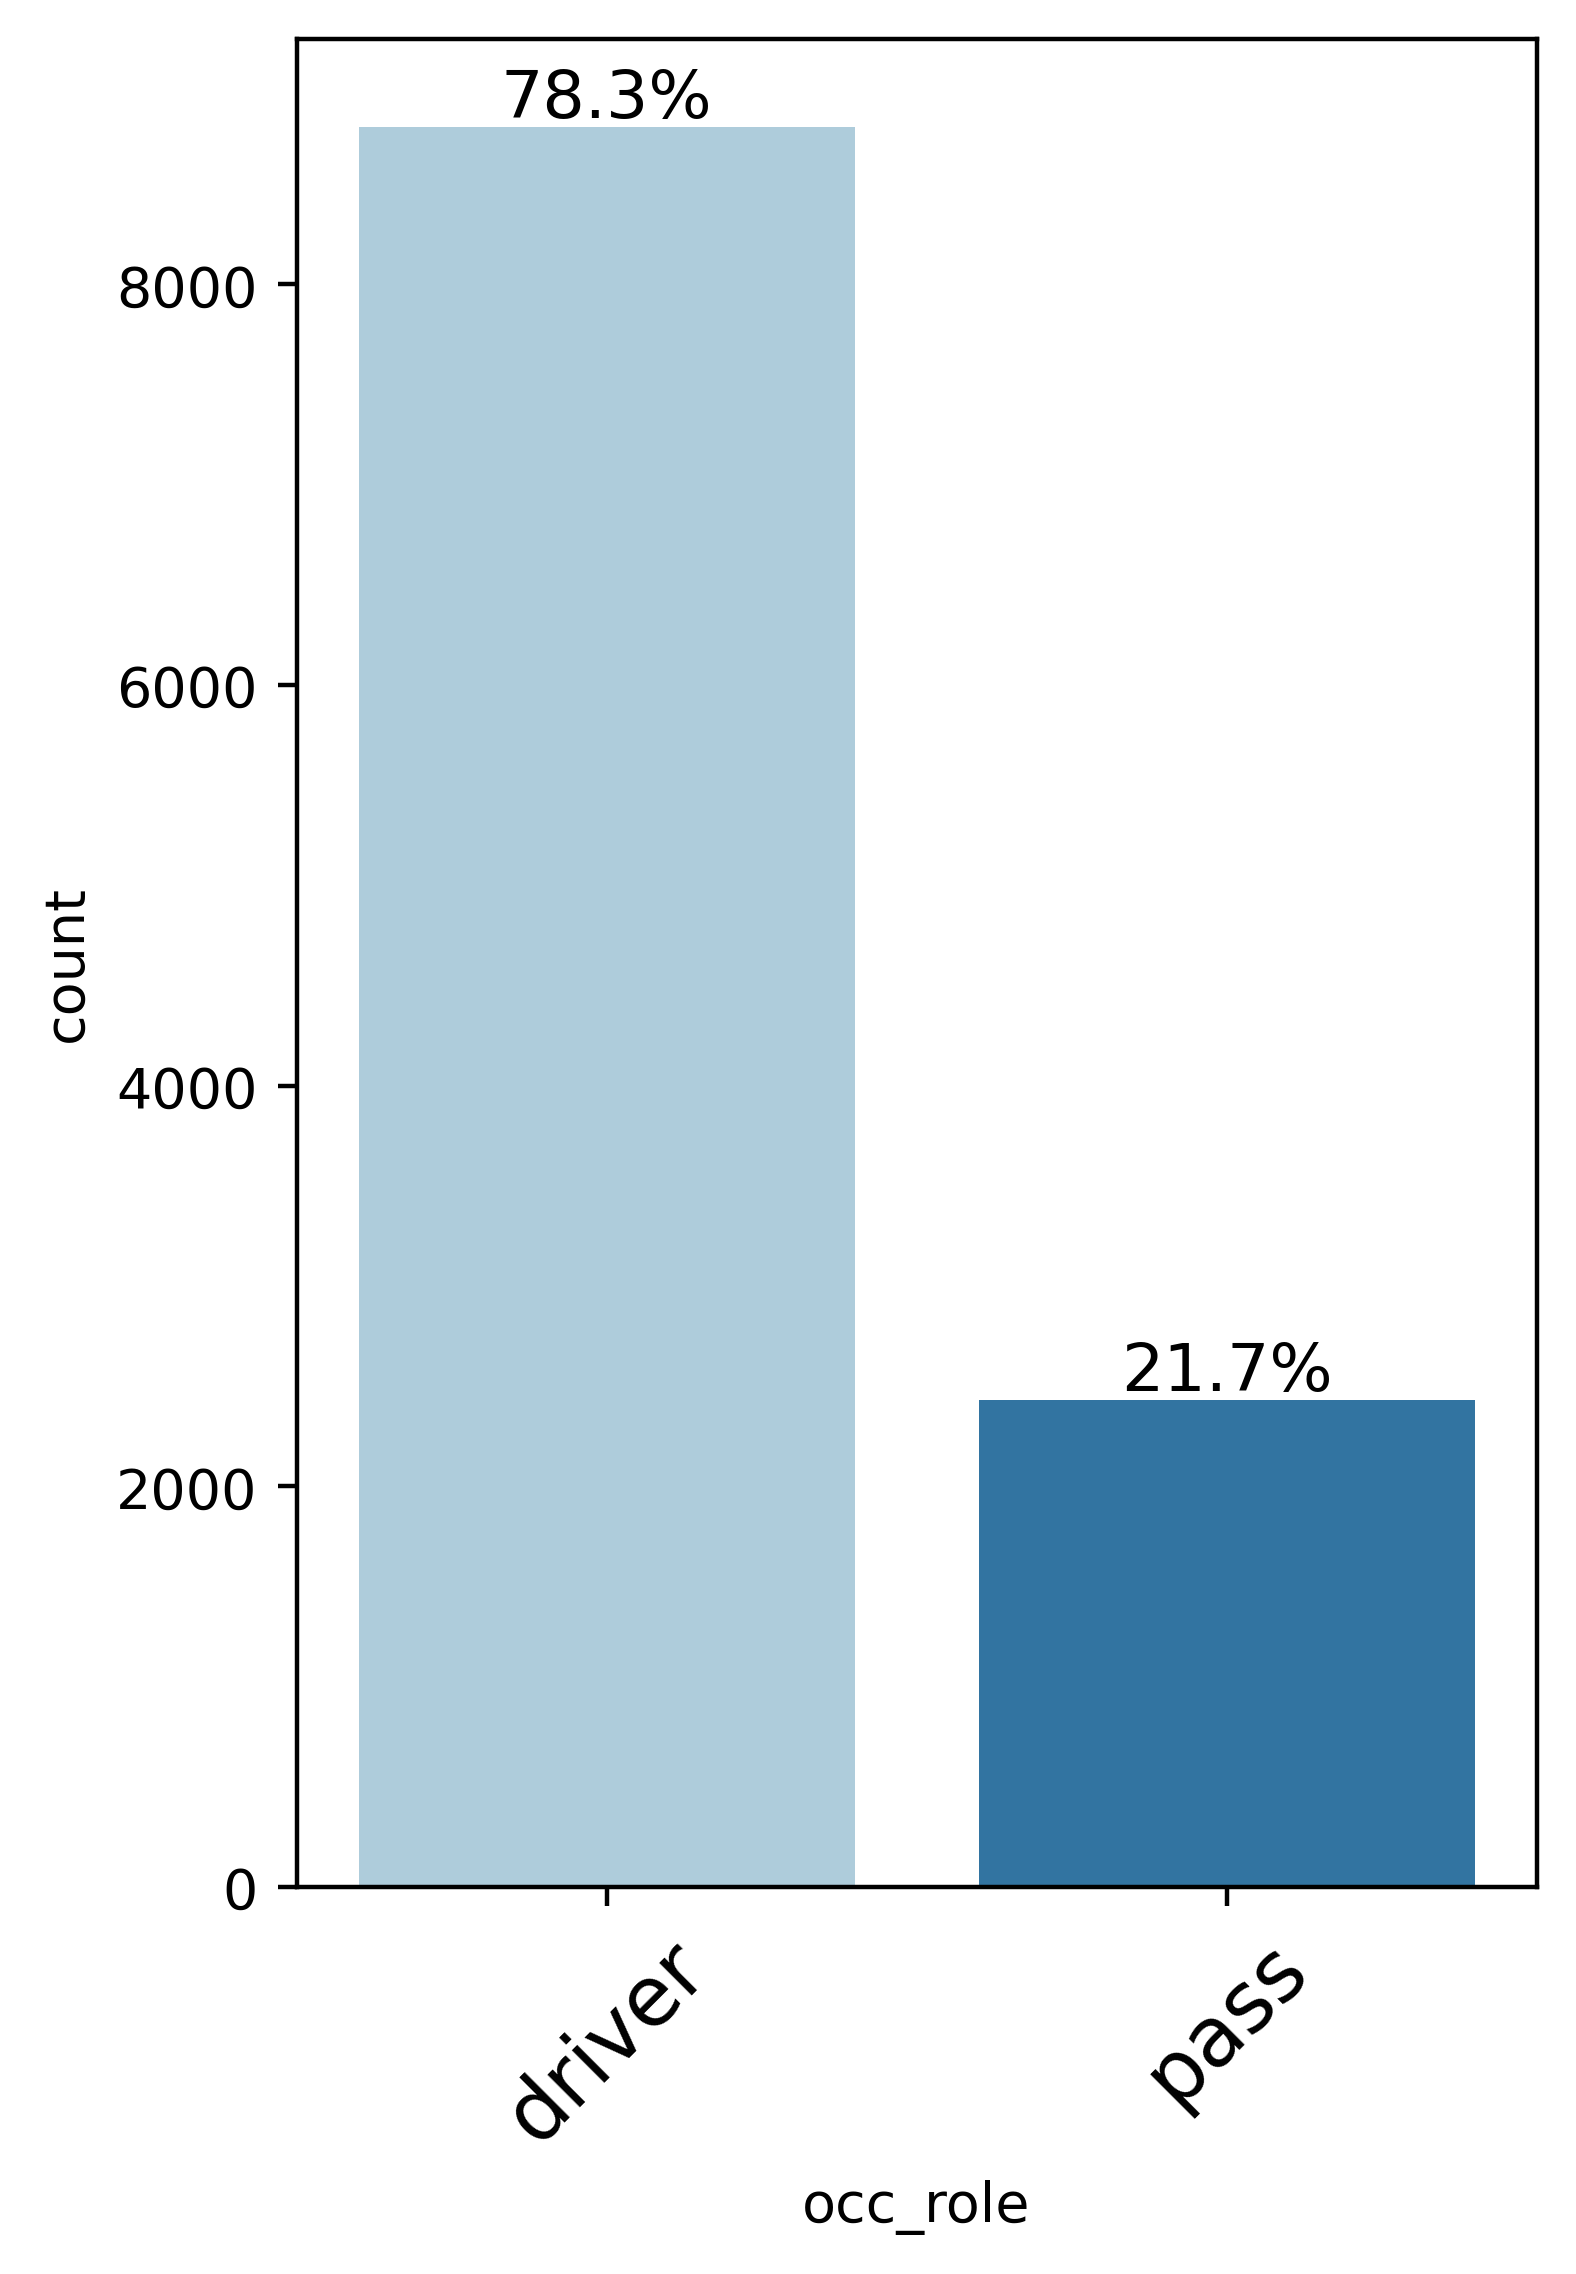
\includegraphics[width=4cm]{occ_role_dist.png}
			\caption{}
			\label{fig:occ_role_dist}
		\end{subfigure}
		\hfill
		\begin{subfigure}[t]{0.24\textwidth}
			\centering
			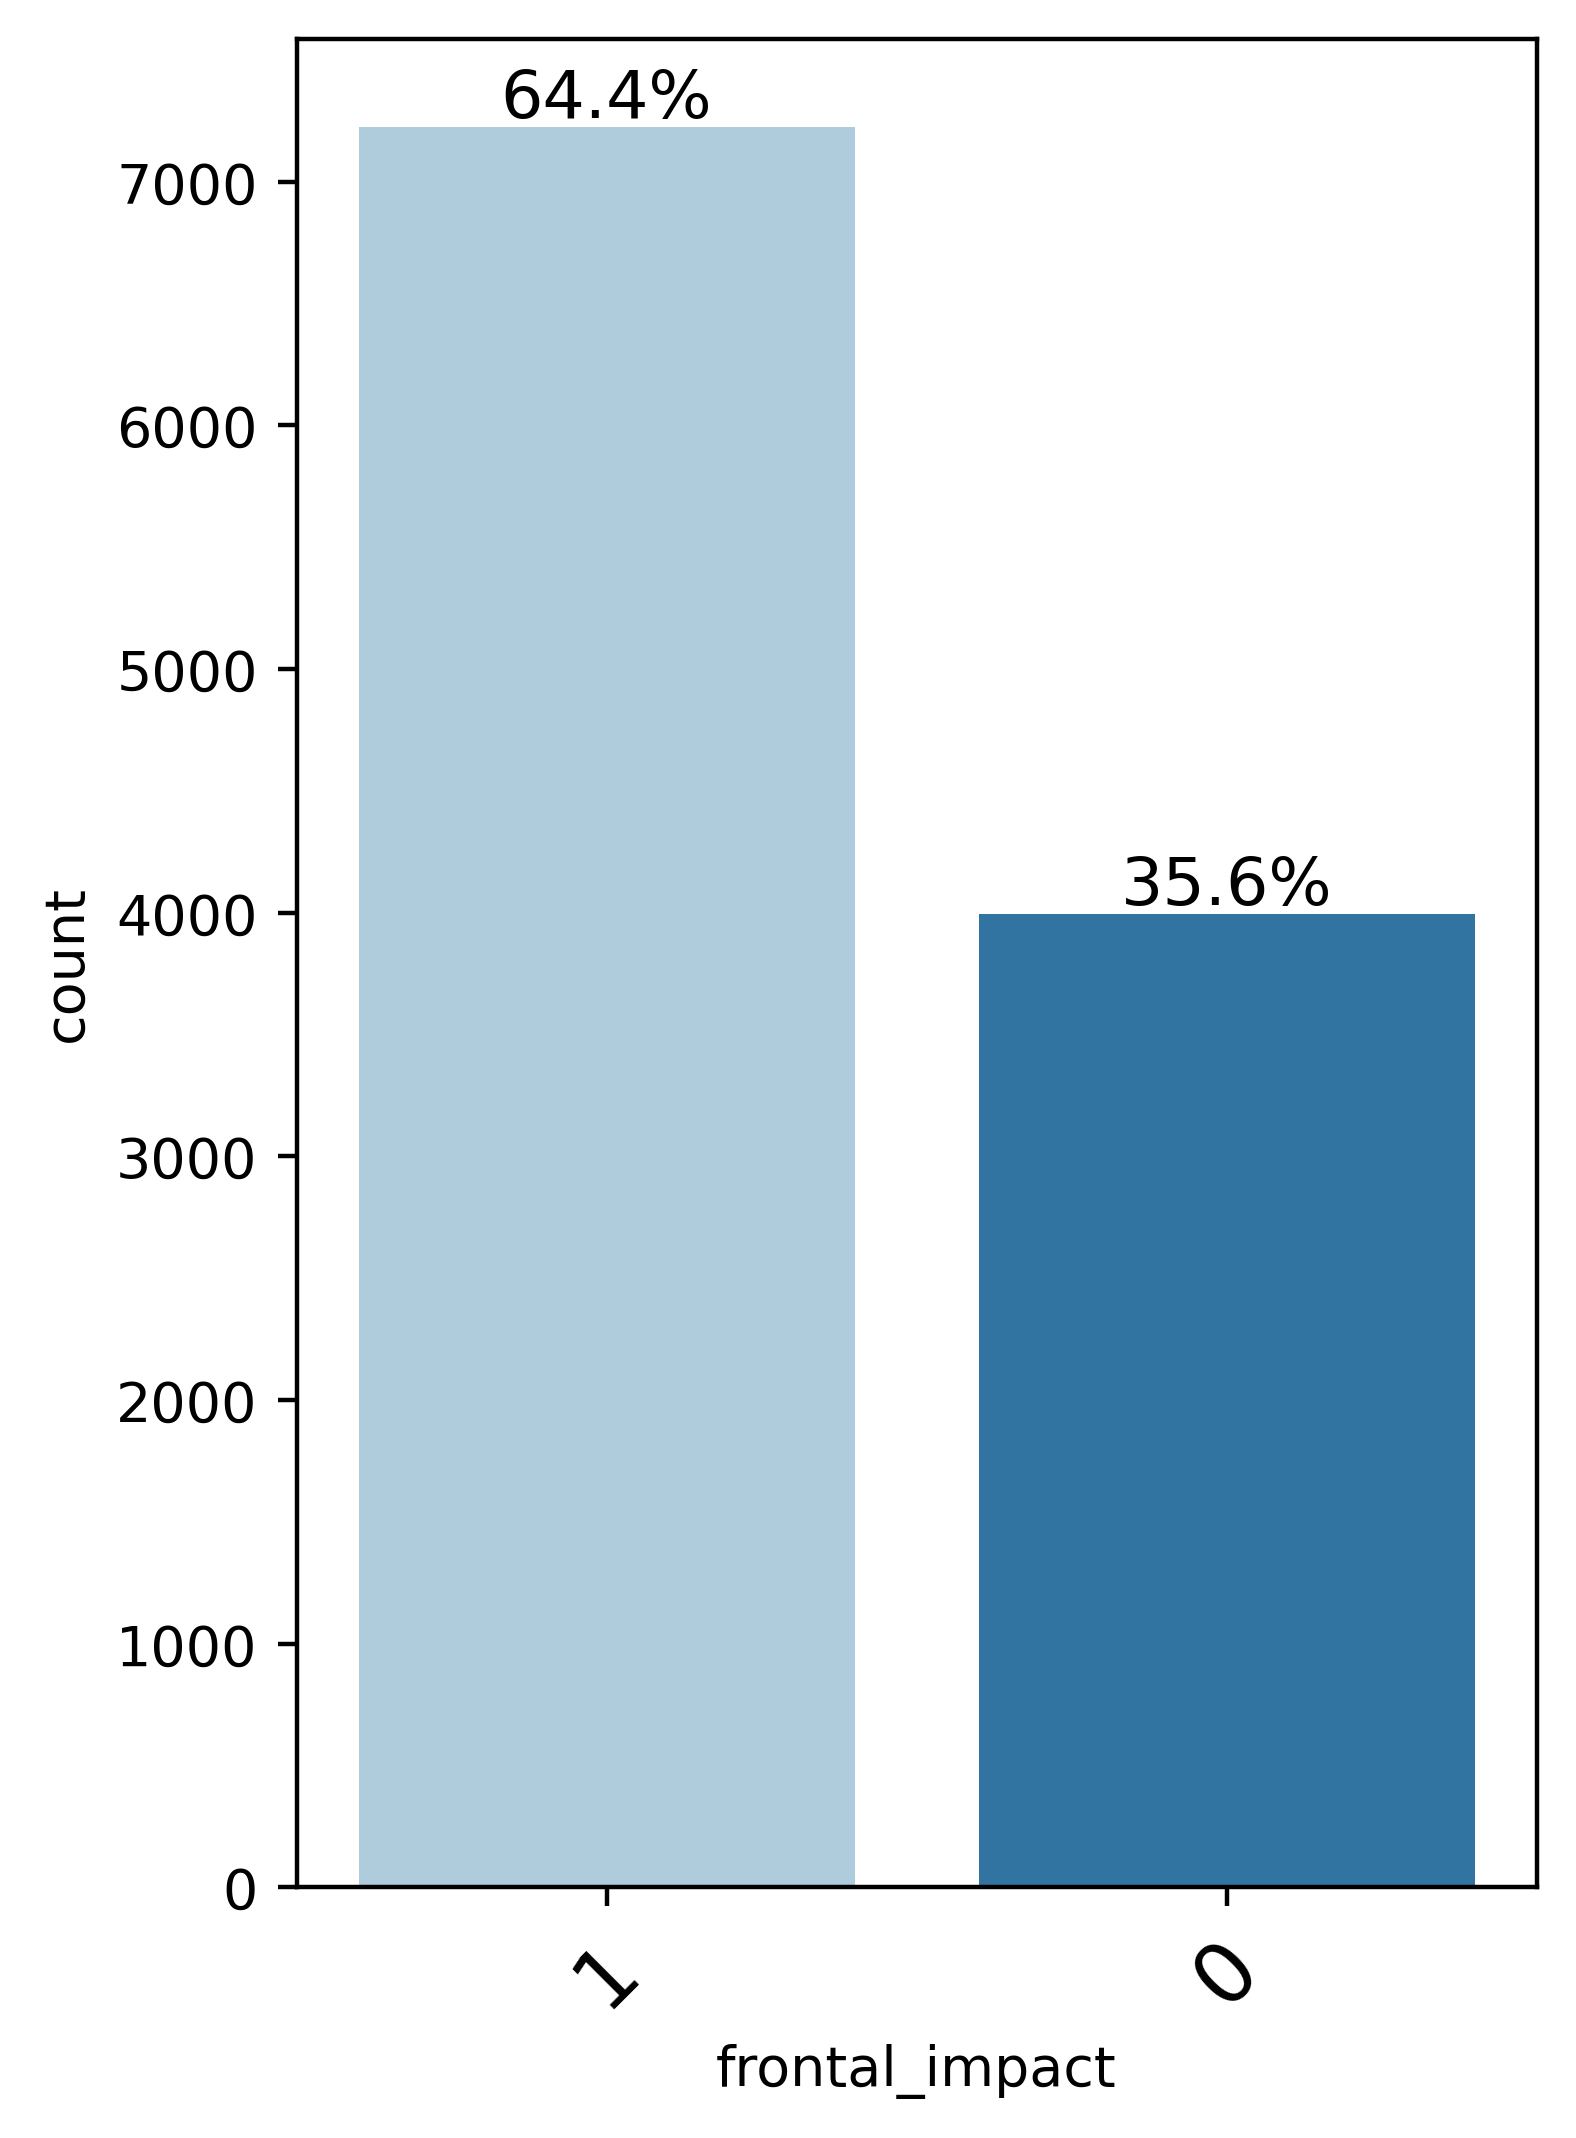
\includegraphics[width=4cm]{frontal_impact_dist.png}
			\caption{}
			\label{fig:frontal_impact_dist}
		\end{subfigure}
		\hfill
		\begin{subfigure}[t]{0.35\textwidth}
			\centering
			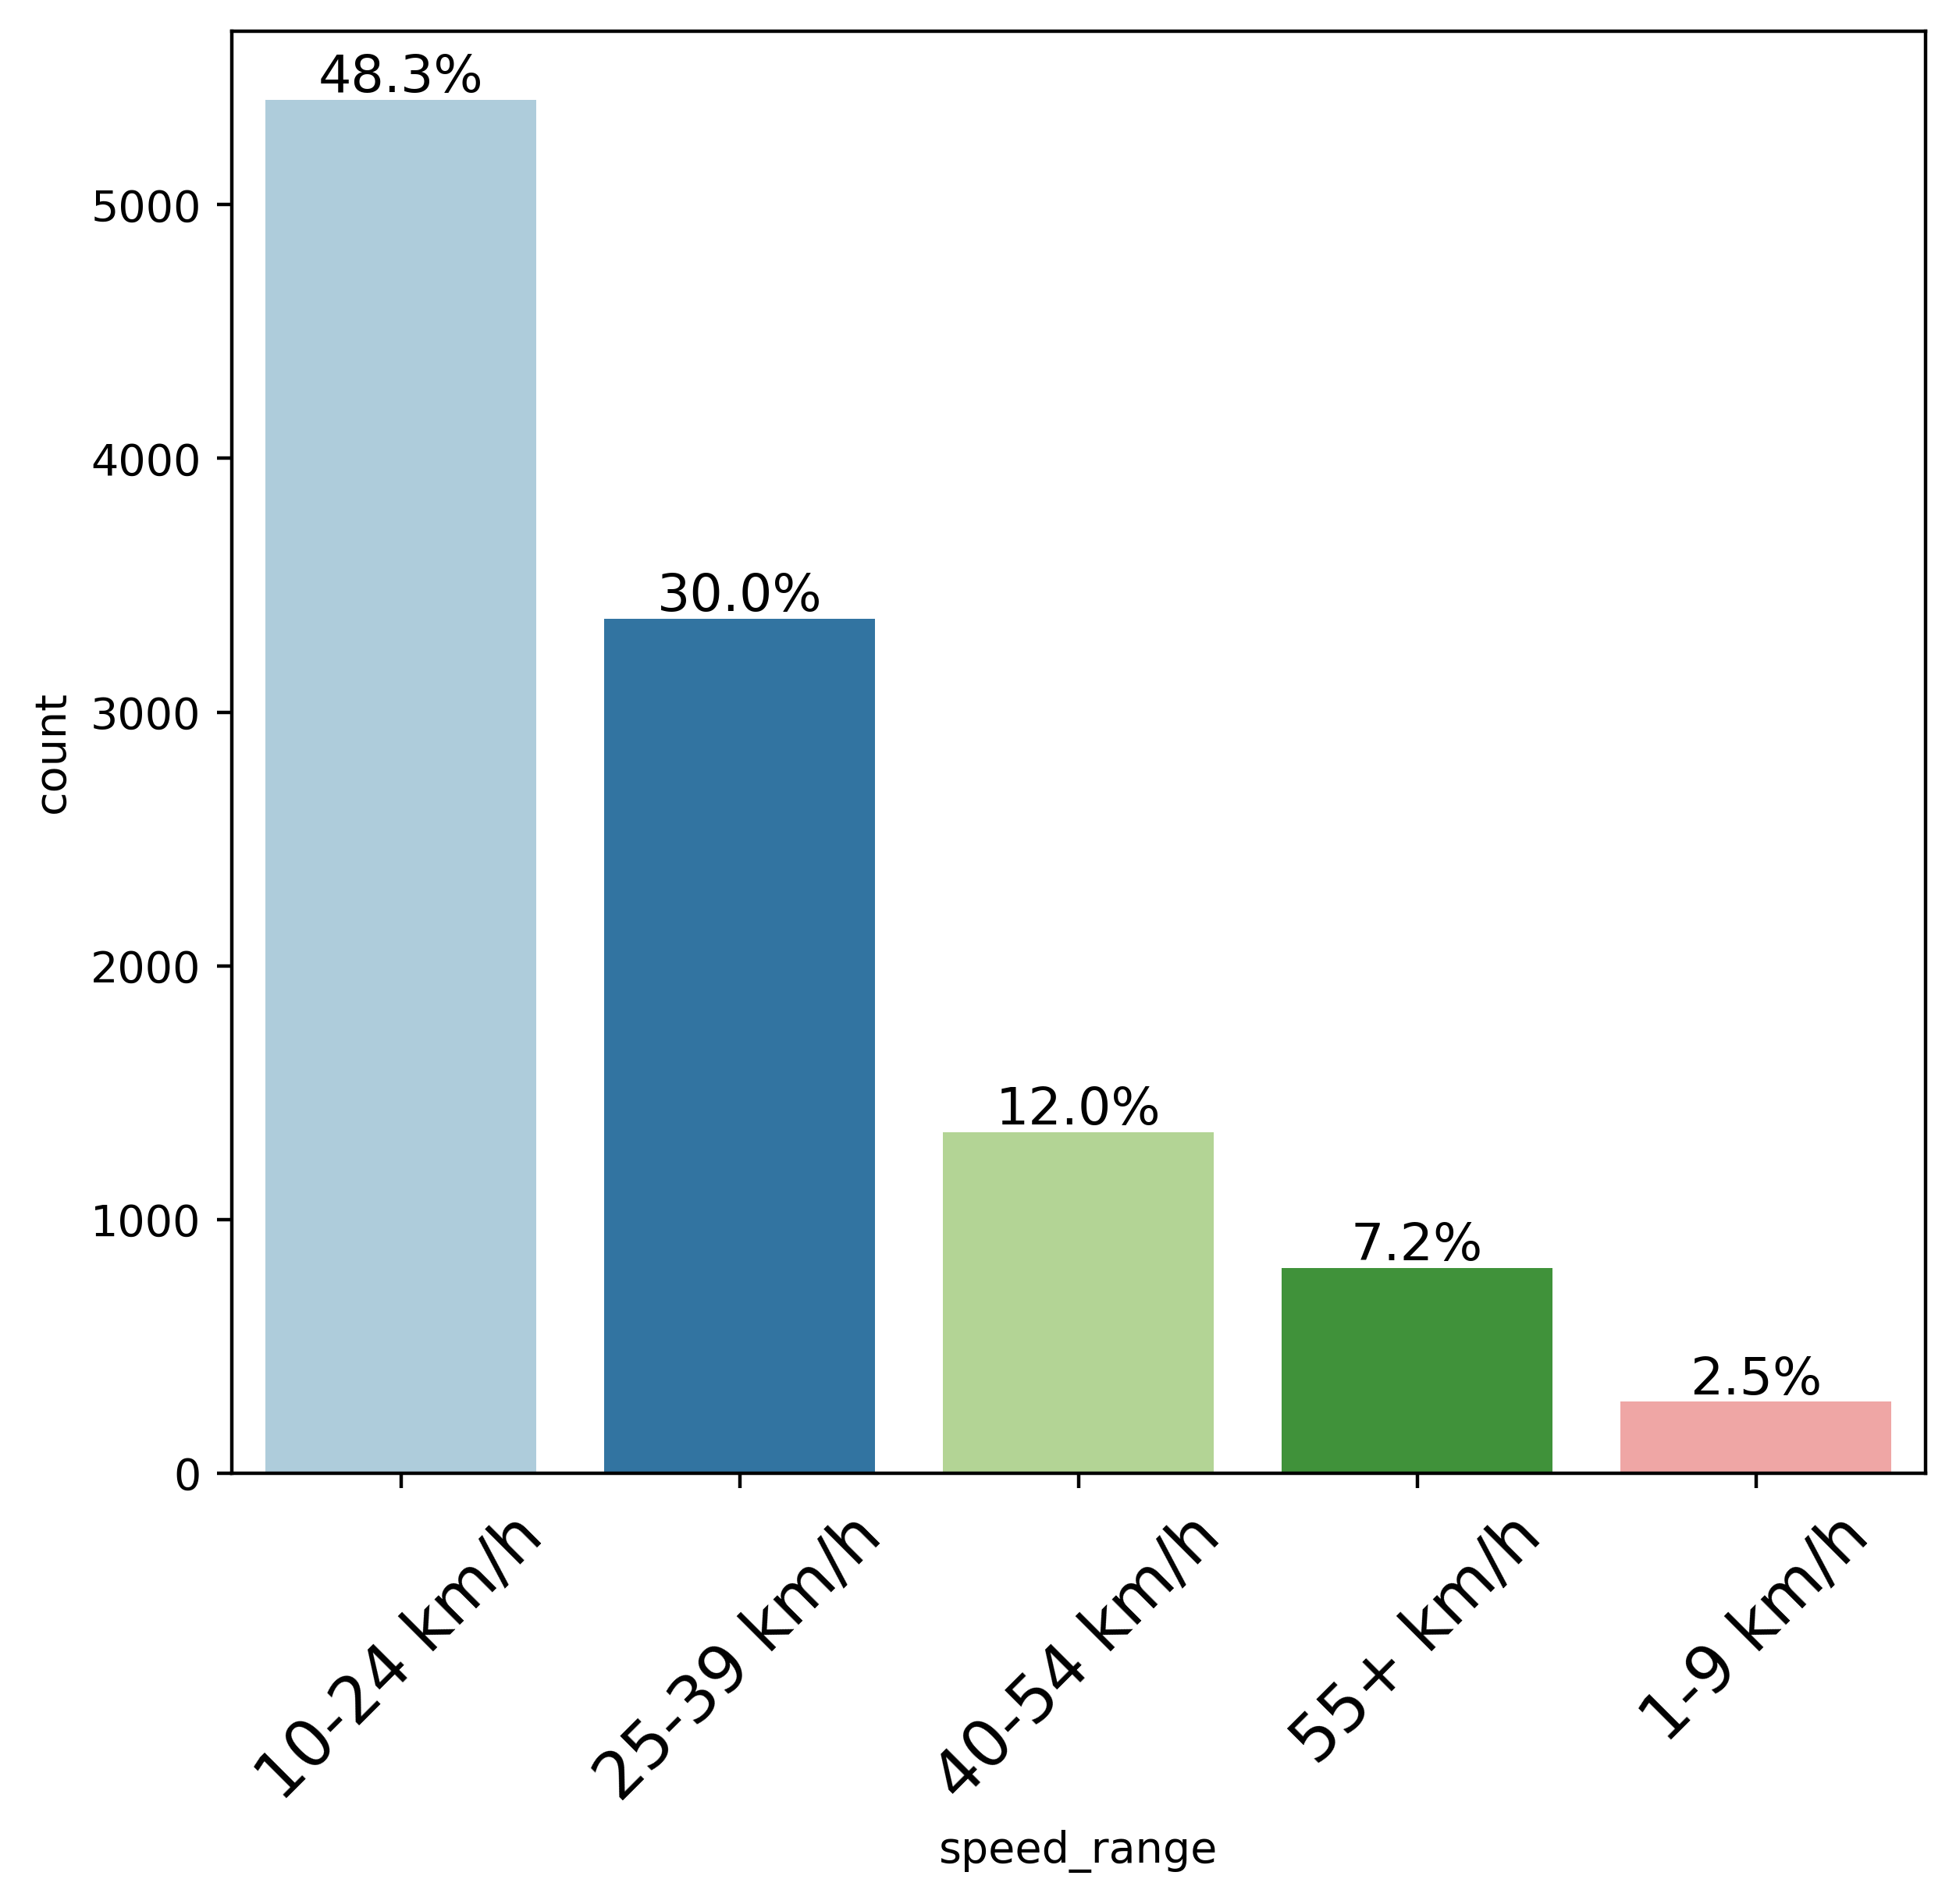
\includegraphics[width=7cm]{speed_dist.png}
			\caption{}
			\label{fig:speed_dist}
		\end{subfigure}
		\hfill
		\begin{subfigure}[t]{0.35\textwidth}
			\centering
			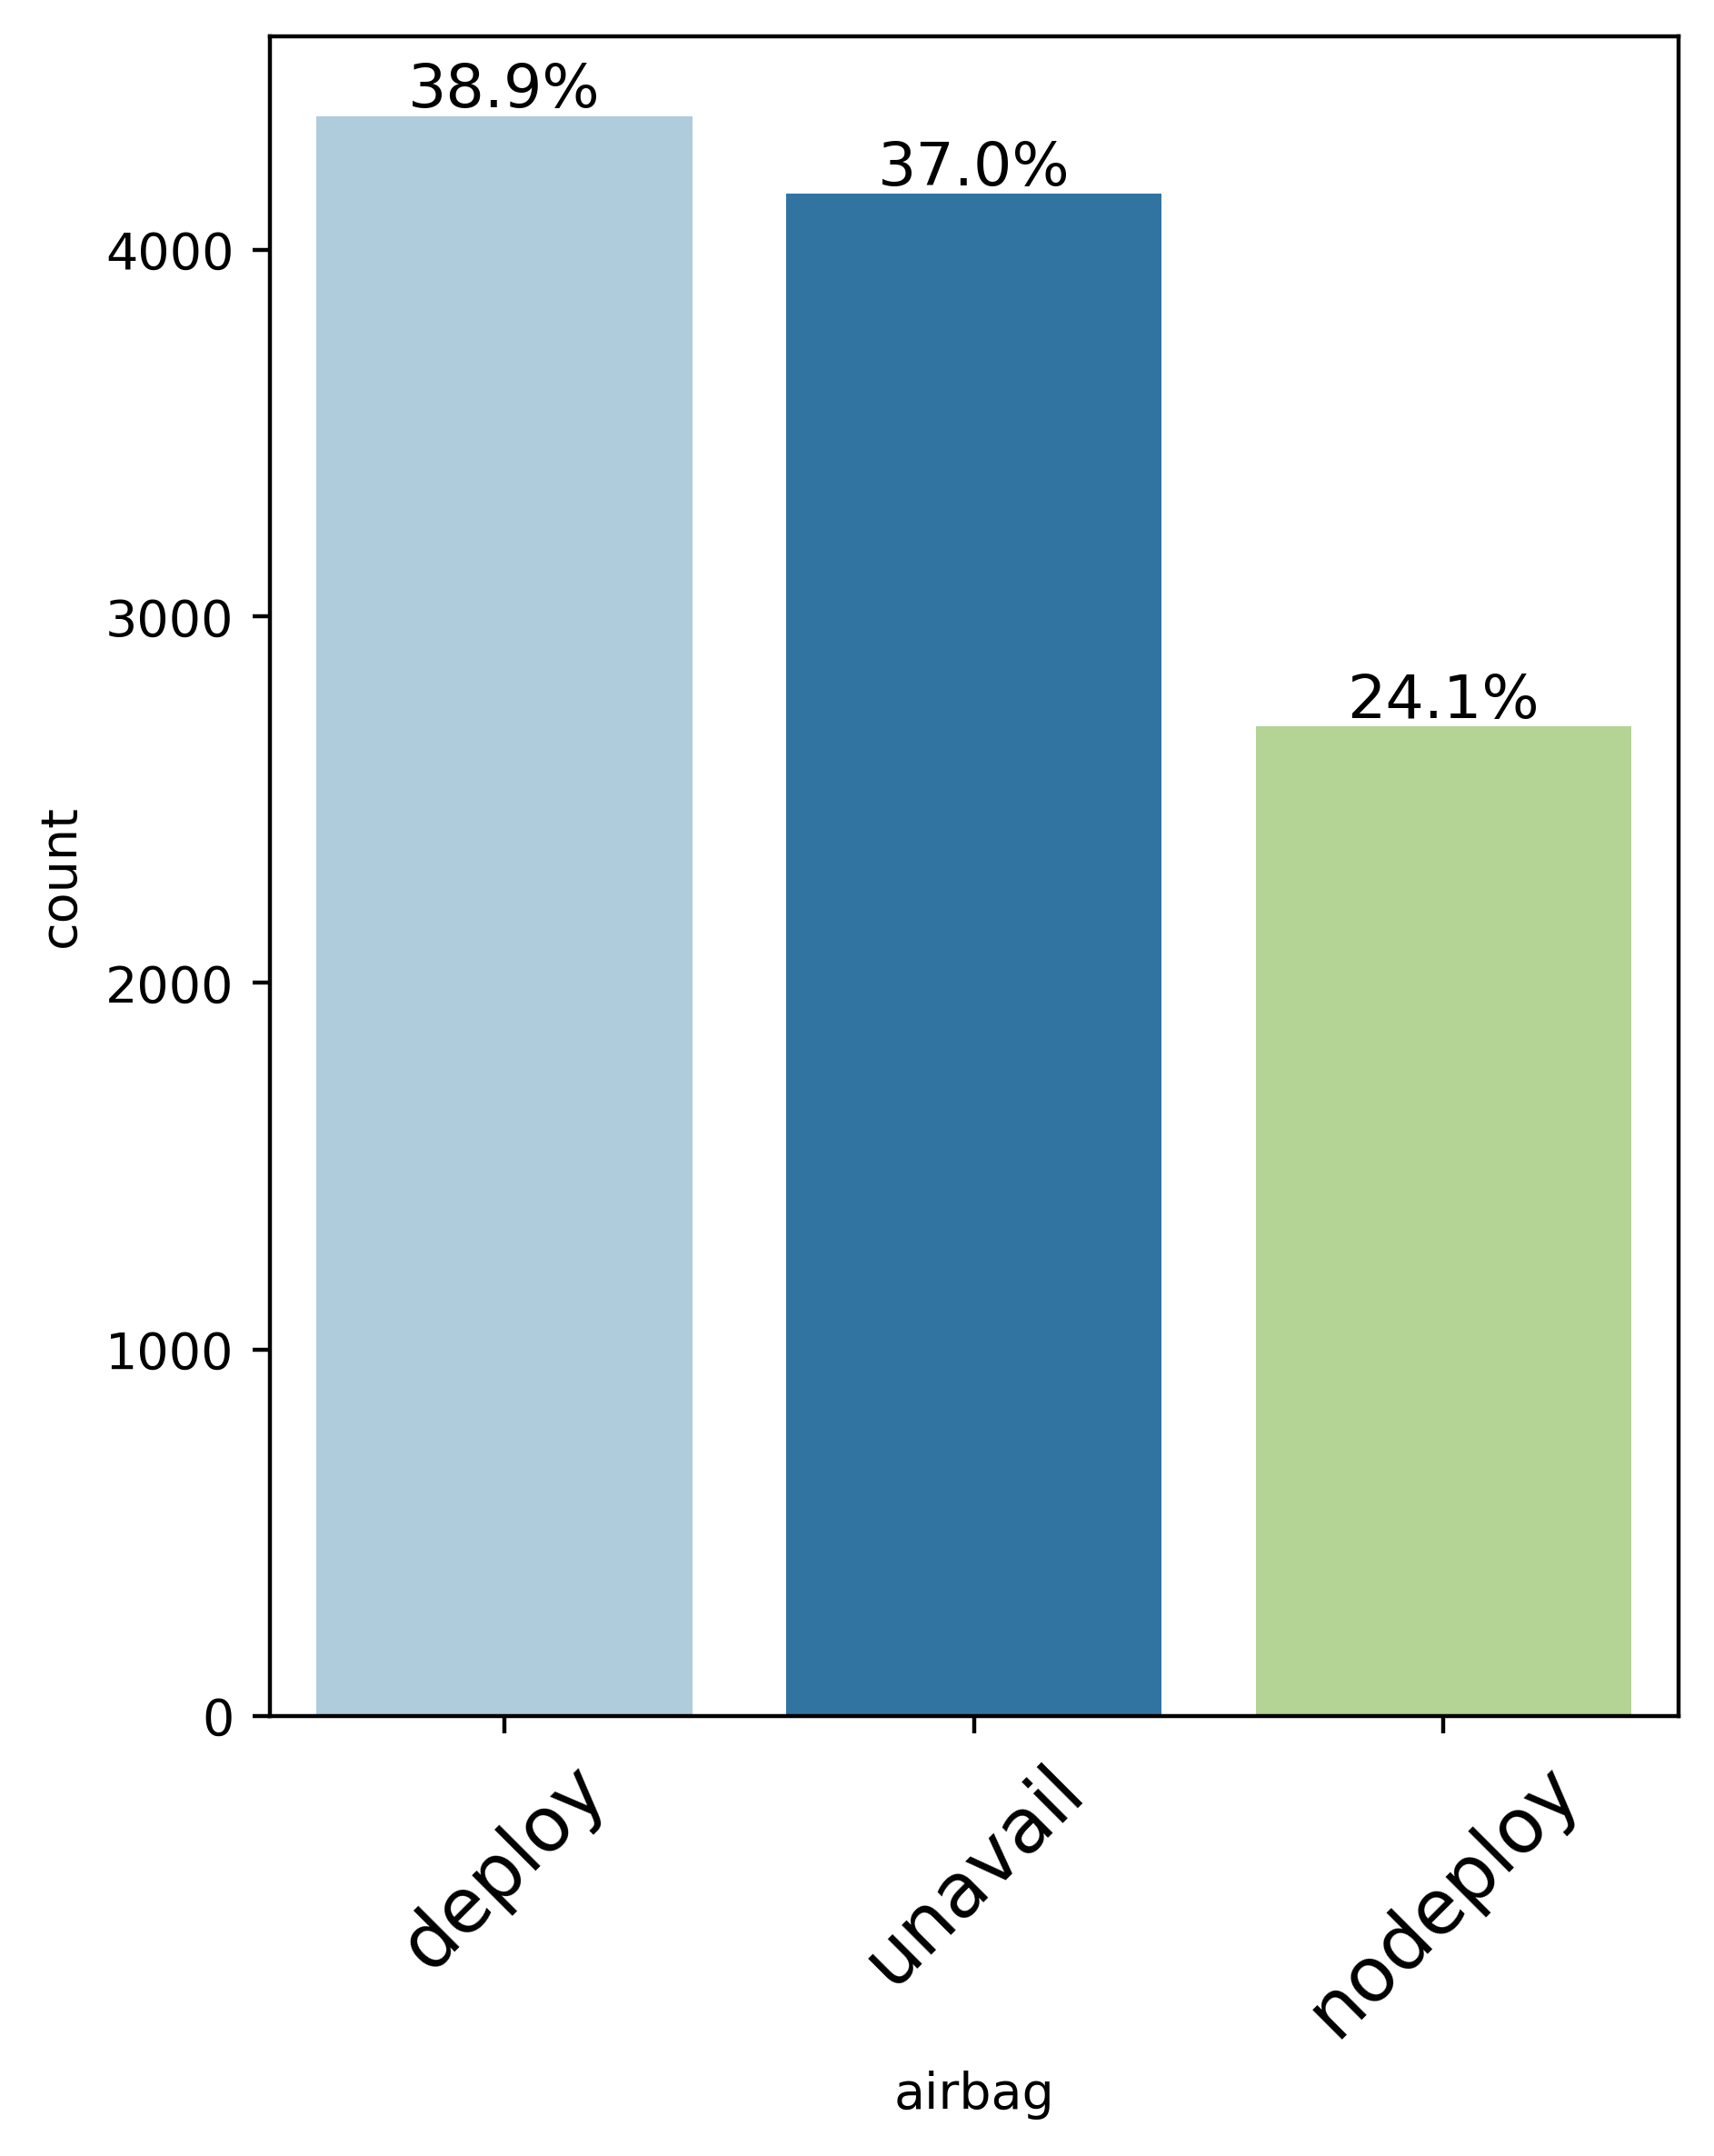
\includegraphics[width=5cm]{airbag_dist.png}
			\caption{}
			\label{fig:airbag_dist}
		\end{subfigure}
		\caption{Distribution of Categorical variables}
		\label{fig: Distribution of Categorcal variables }
	\end{figure}	
	Figure \ref{fig: Distribution of Categorcal variables } shows the countplots for the distribution of categorical variables. In our data set 89.5 \% of occupants survived the accidents. 53.9\% of occupants are males. Around 30\% of occupants were not belted while the accidents occurred. More than 70\% of the occupants are drivers. Among the accidents more than 64 \% of occupants had a frontal impact injury. Approximately 39\% of vehicles were traveling at speeds exceeding 25 km/h, while 7\% were moving at speeds over 55 km/h.In over 60\% of cases, the airbag either did not deploy or was unavailable.
	\begin{figure}[h]
		\centering
		\begin{subfigure}[t]{0.495\linewidth}
			\centering
			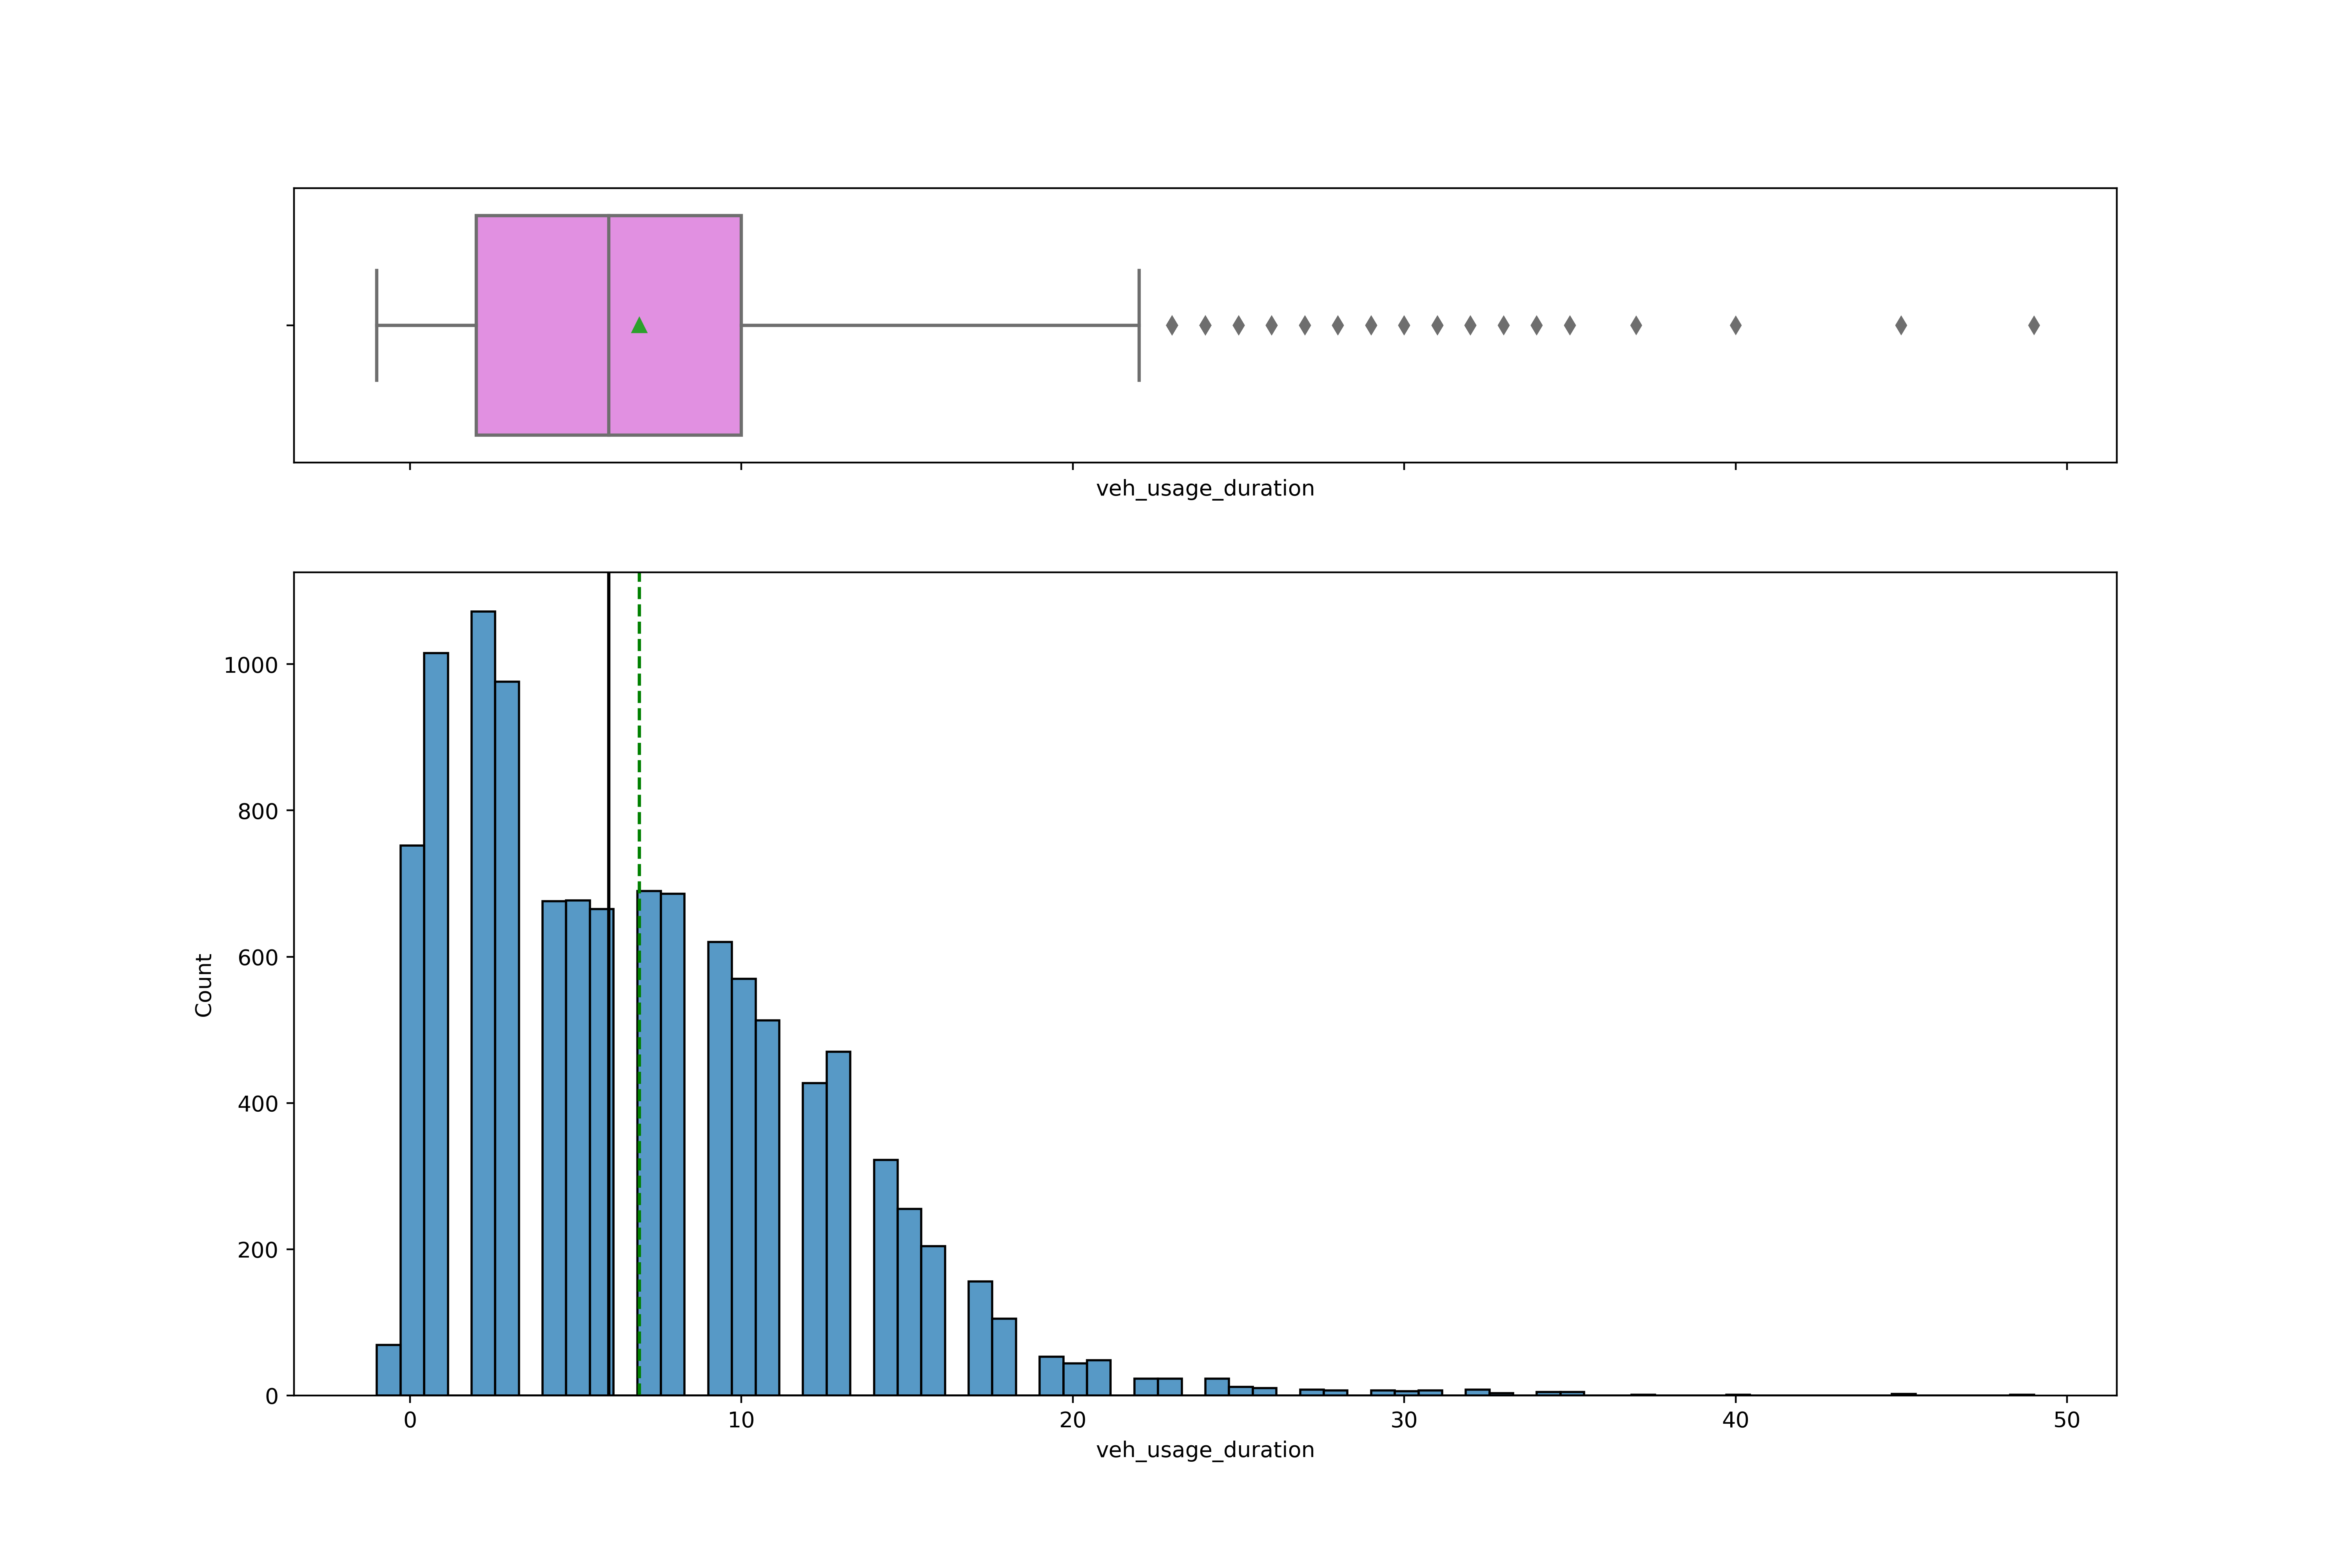
\includegraphics[width=\linewidth]{veh_duration_dist.png}
			\caption{Histogram and boxplot of vehicle usage duration}
			\label{fig:veh_duration_dist}
		\end{subfigure}
		\hfill
		\begin{subfigure}[t]{0.495\linewidth}
			\centering
			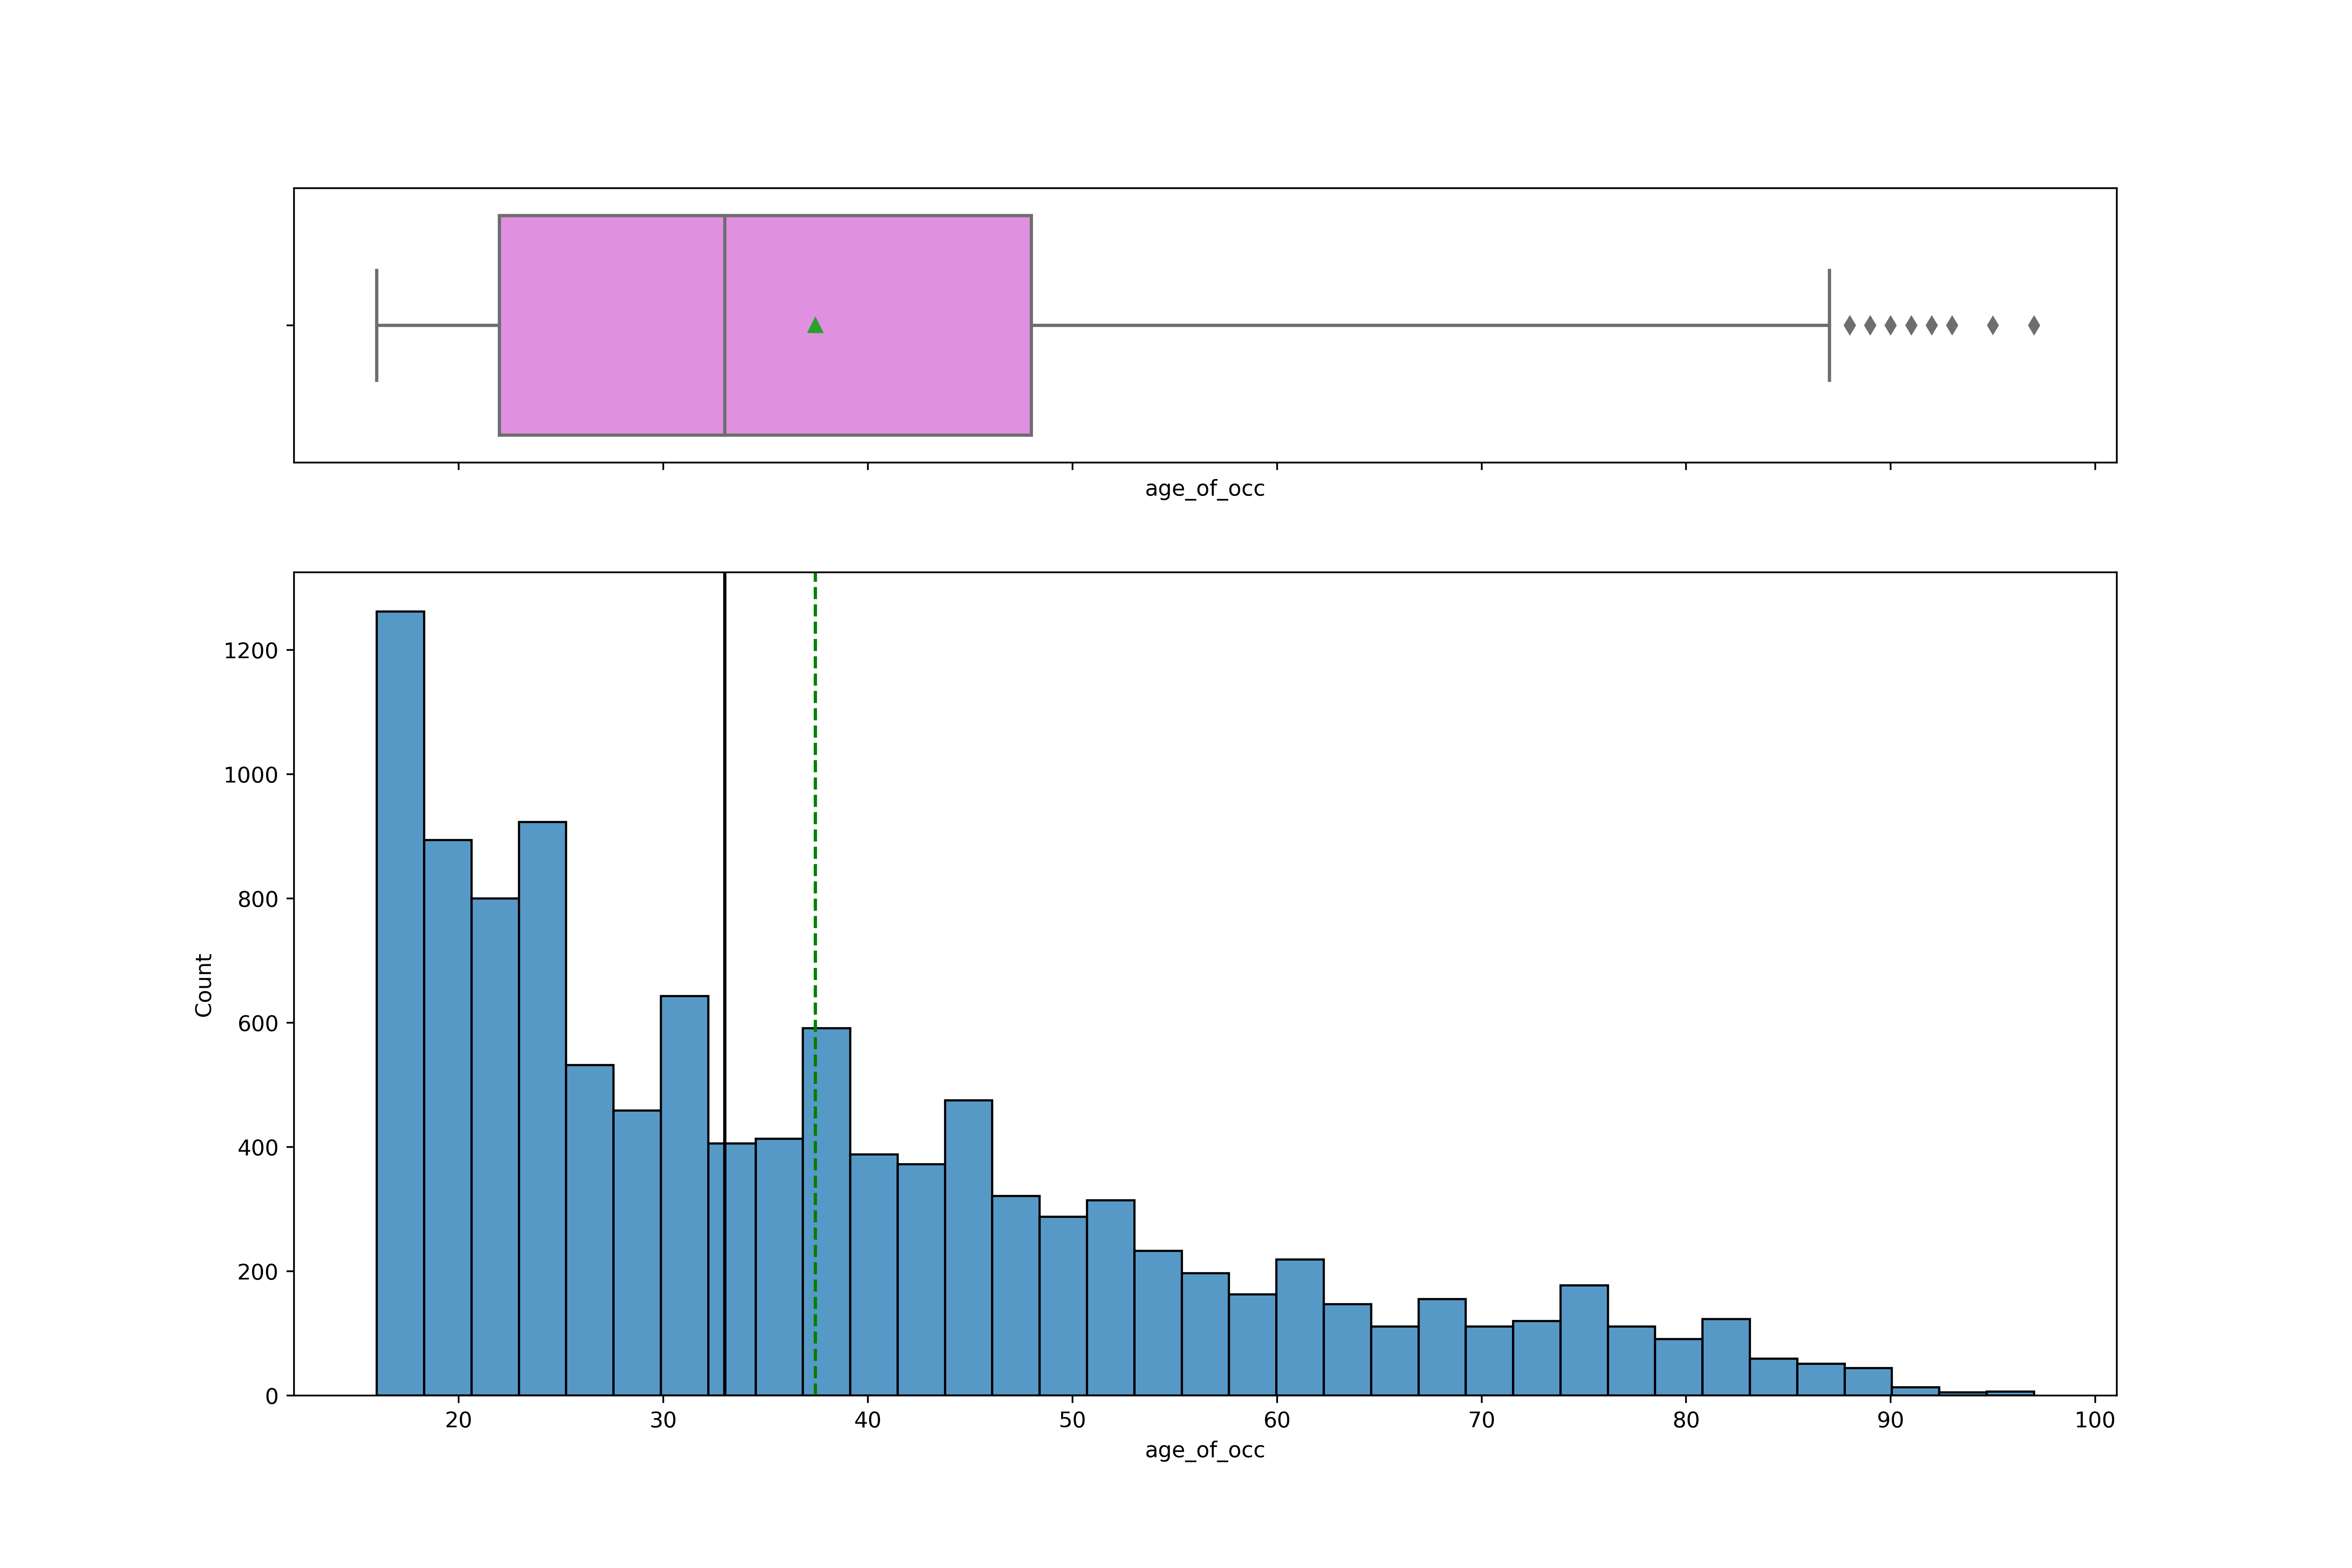
\includegraphics[width=\linewidth]{age_dist.png}
			\caption{Histogram and boxplot of person's age}
			\label{fig:age_dist}
		\end{subfigure}
		\caption{Distribution of numerical variables}
		\label{fig: Distribution of numerical variables }
	\end{figure}
Figure  \ref{fig: Distribution of numerical variables } shows distribution of numerical variables. We observe in figure \ref{fig:veh_duration_dist}, the median usage of vehicles before accidents is around 7 years. Figure \ref{fig:age_dist} shows the distribution of age of occupants. The median age is around 32 and 75 \% of occupants have age less than 50.  
	
	\begin{figure}[h]
	\centering
	\begin{subfigure}[t]{0.32\textwidth}
		\centering
		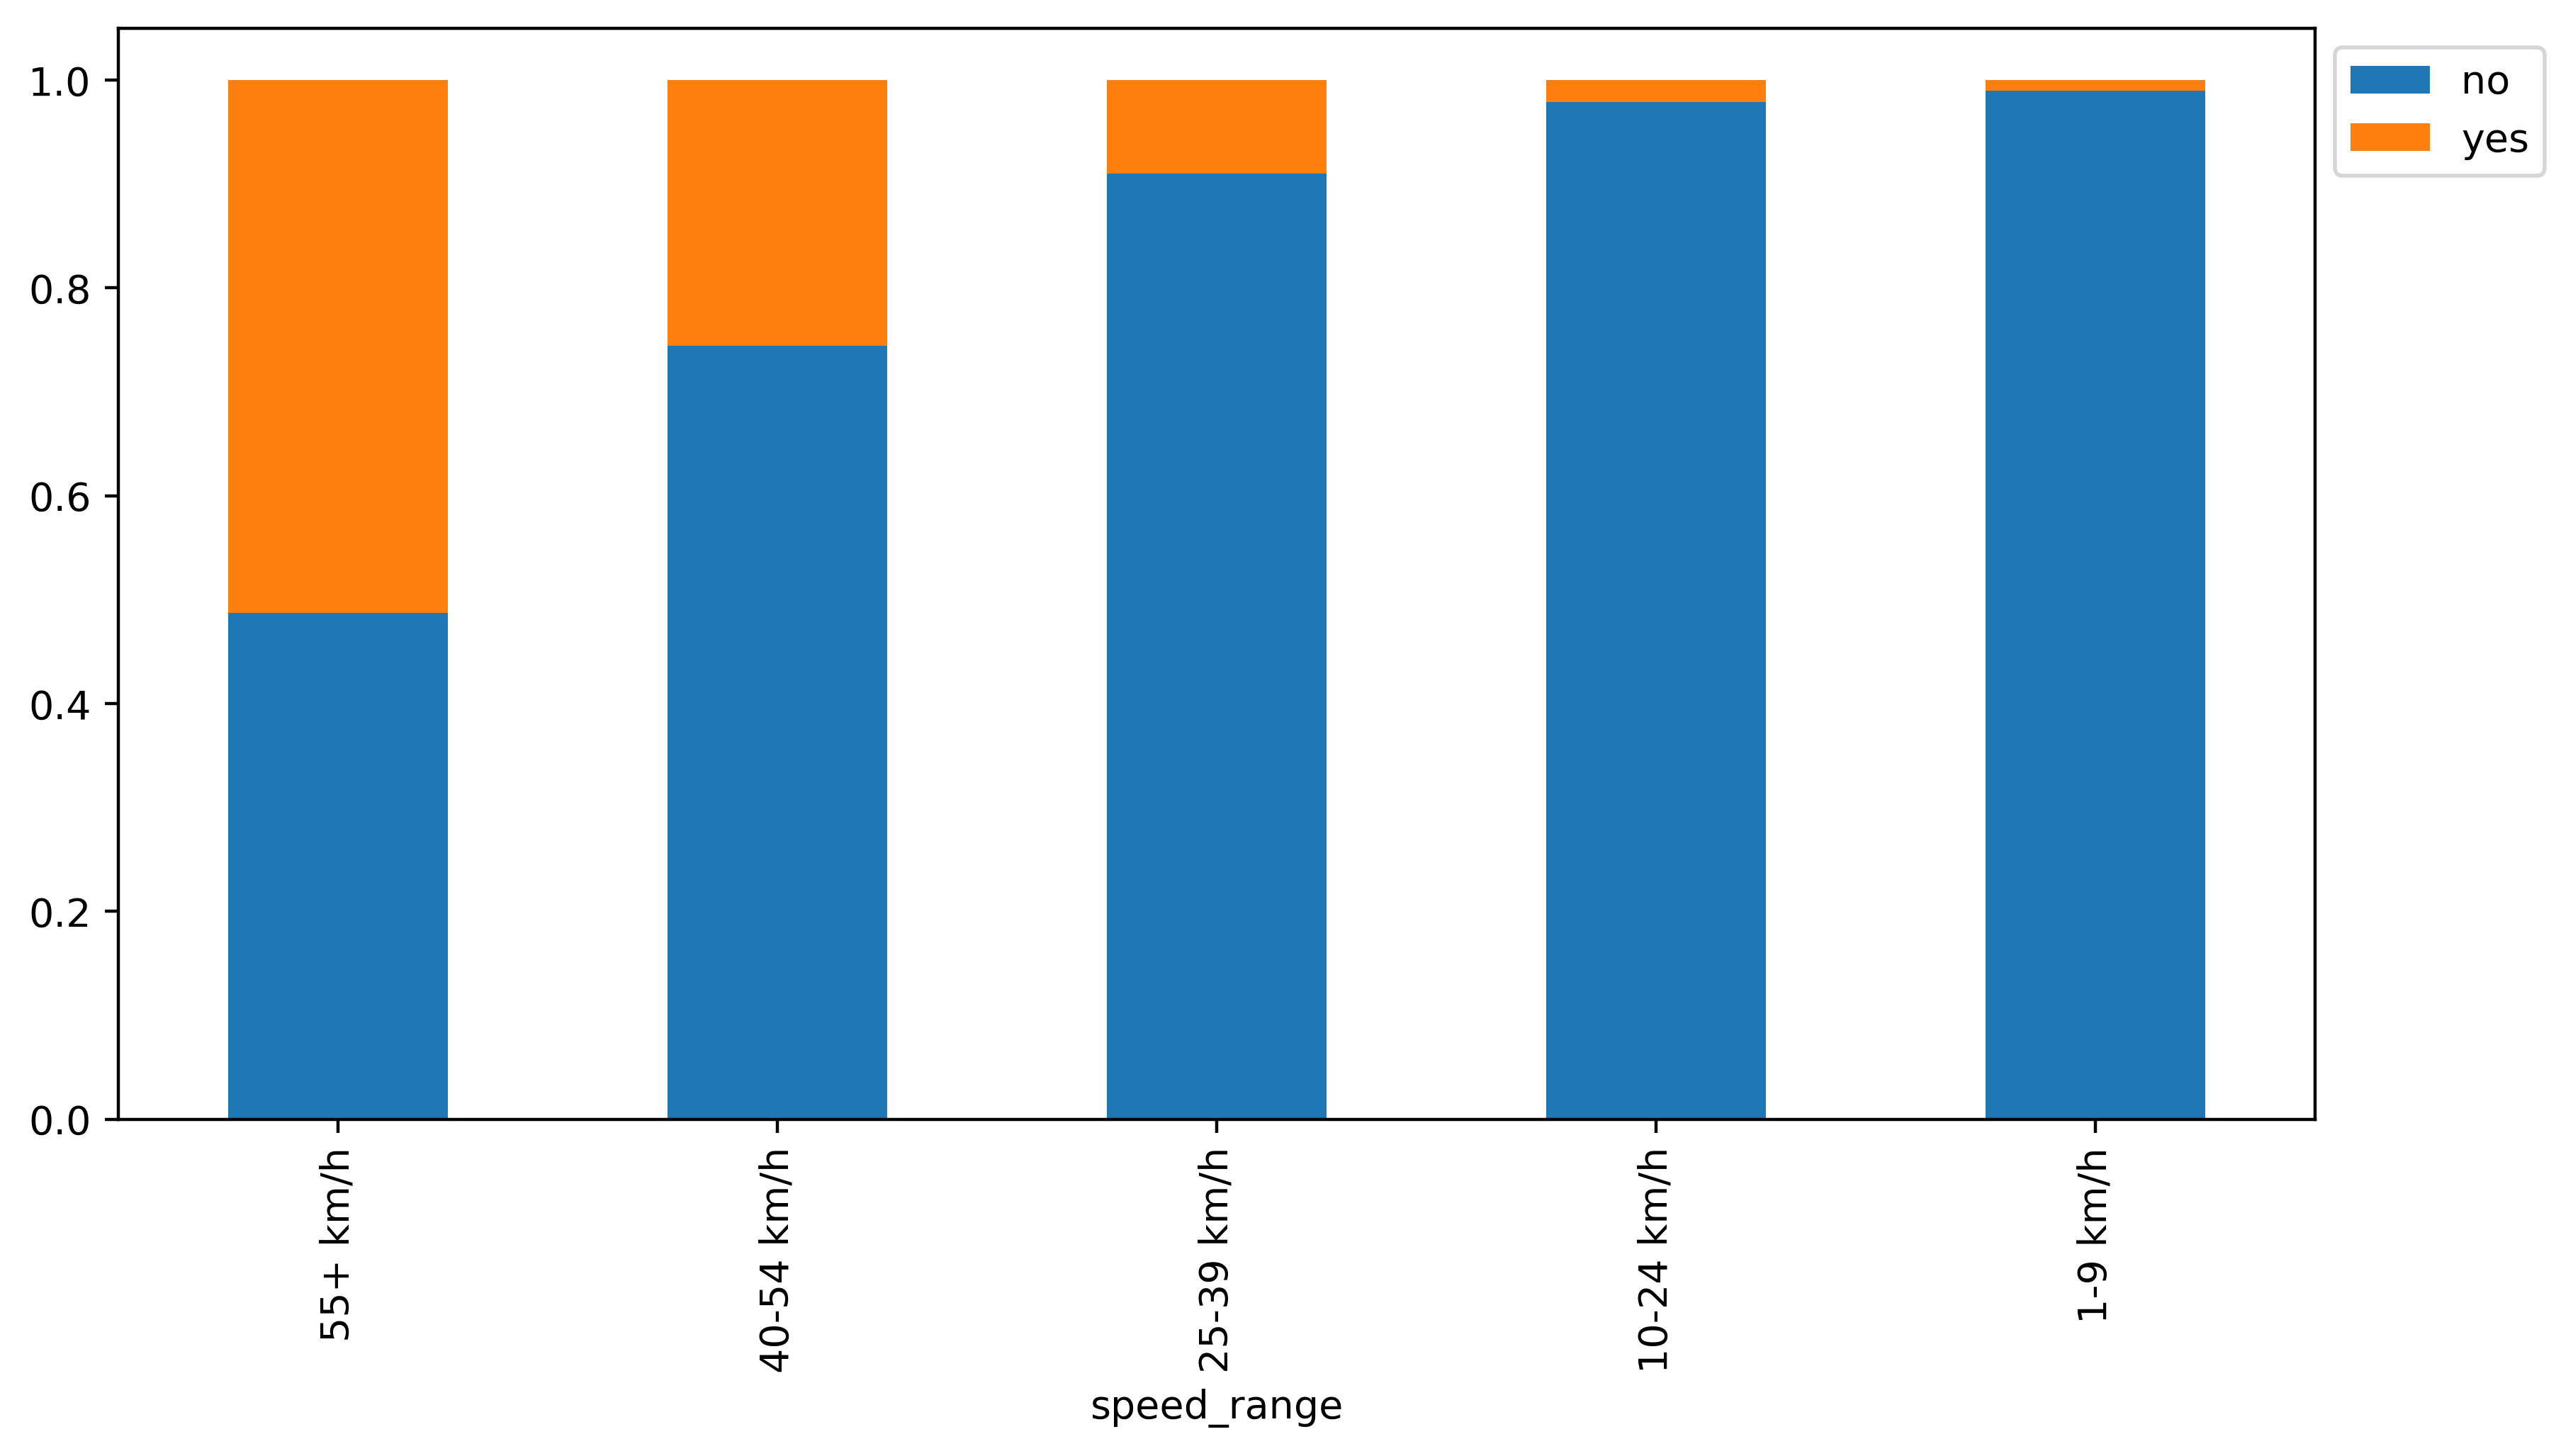
\includegraphics[width=\textwidth]{speed_range_stack_deceased.png}
		\caption{}
		\label{fig:speed_range_stack_deceased}
	\end{subfigure}
	\hfill
	\begin{subfigure}[t]{0.32\textwidth}
		\centering
		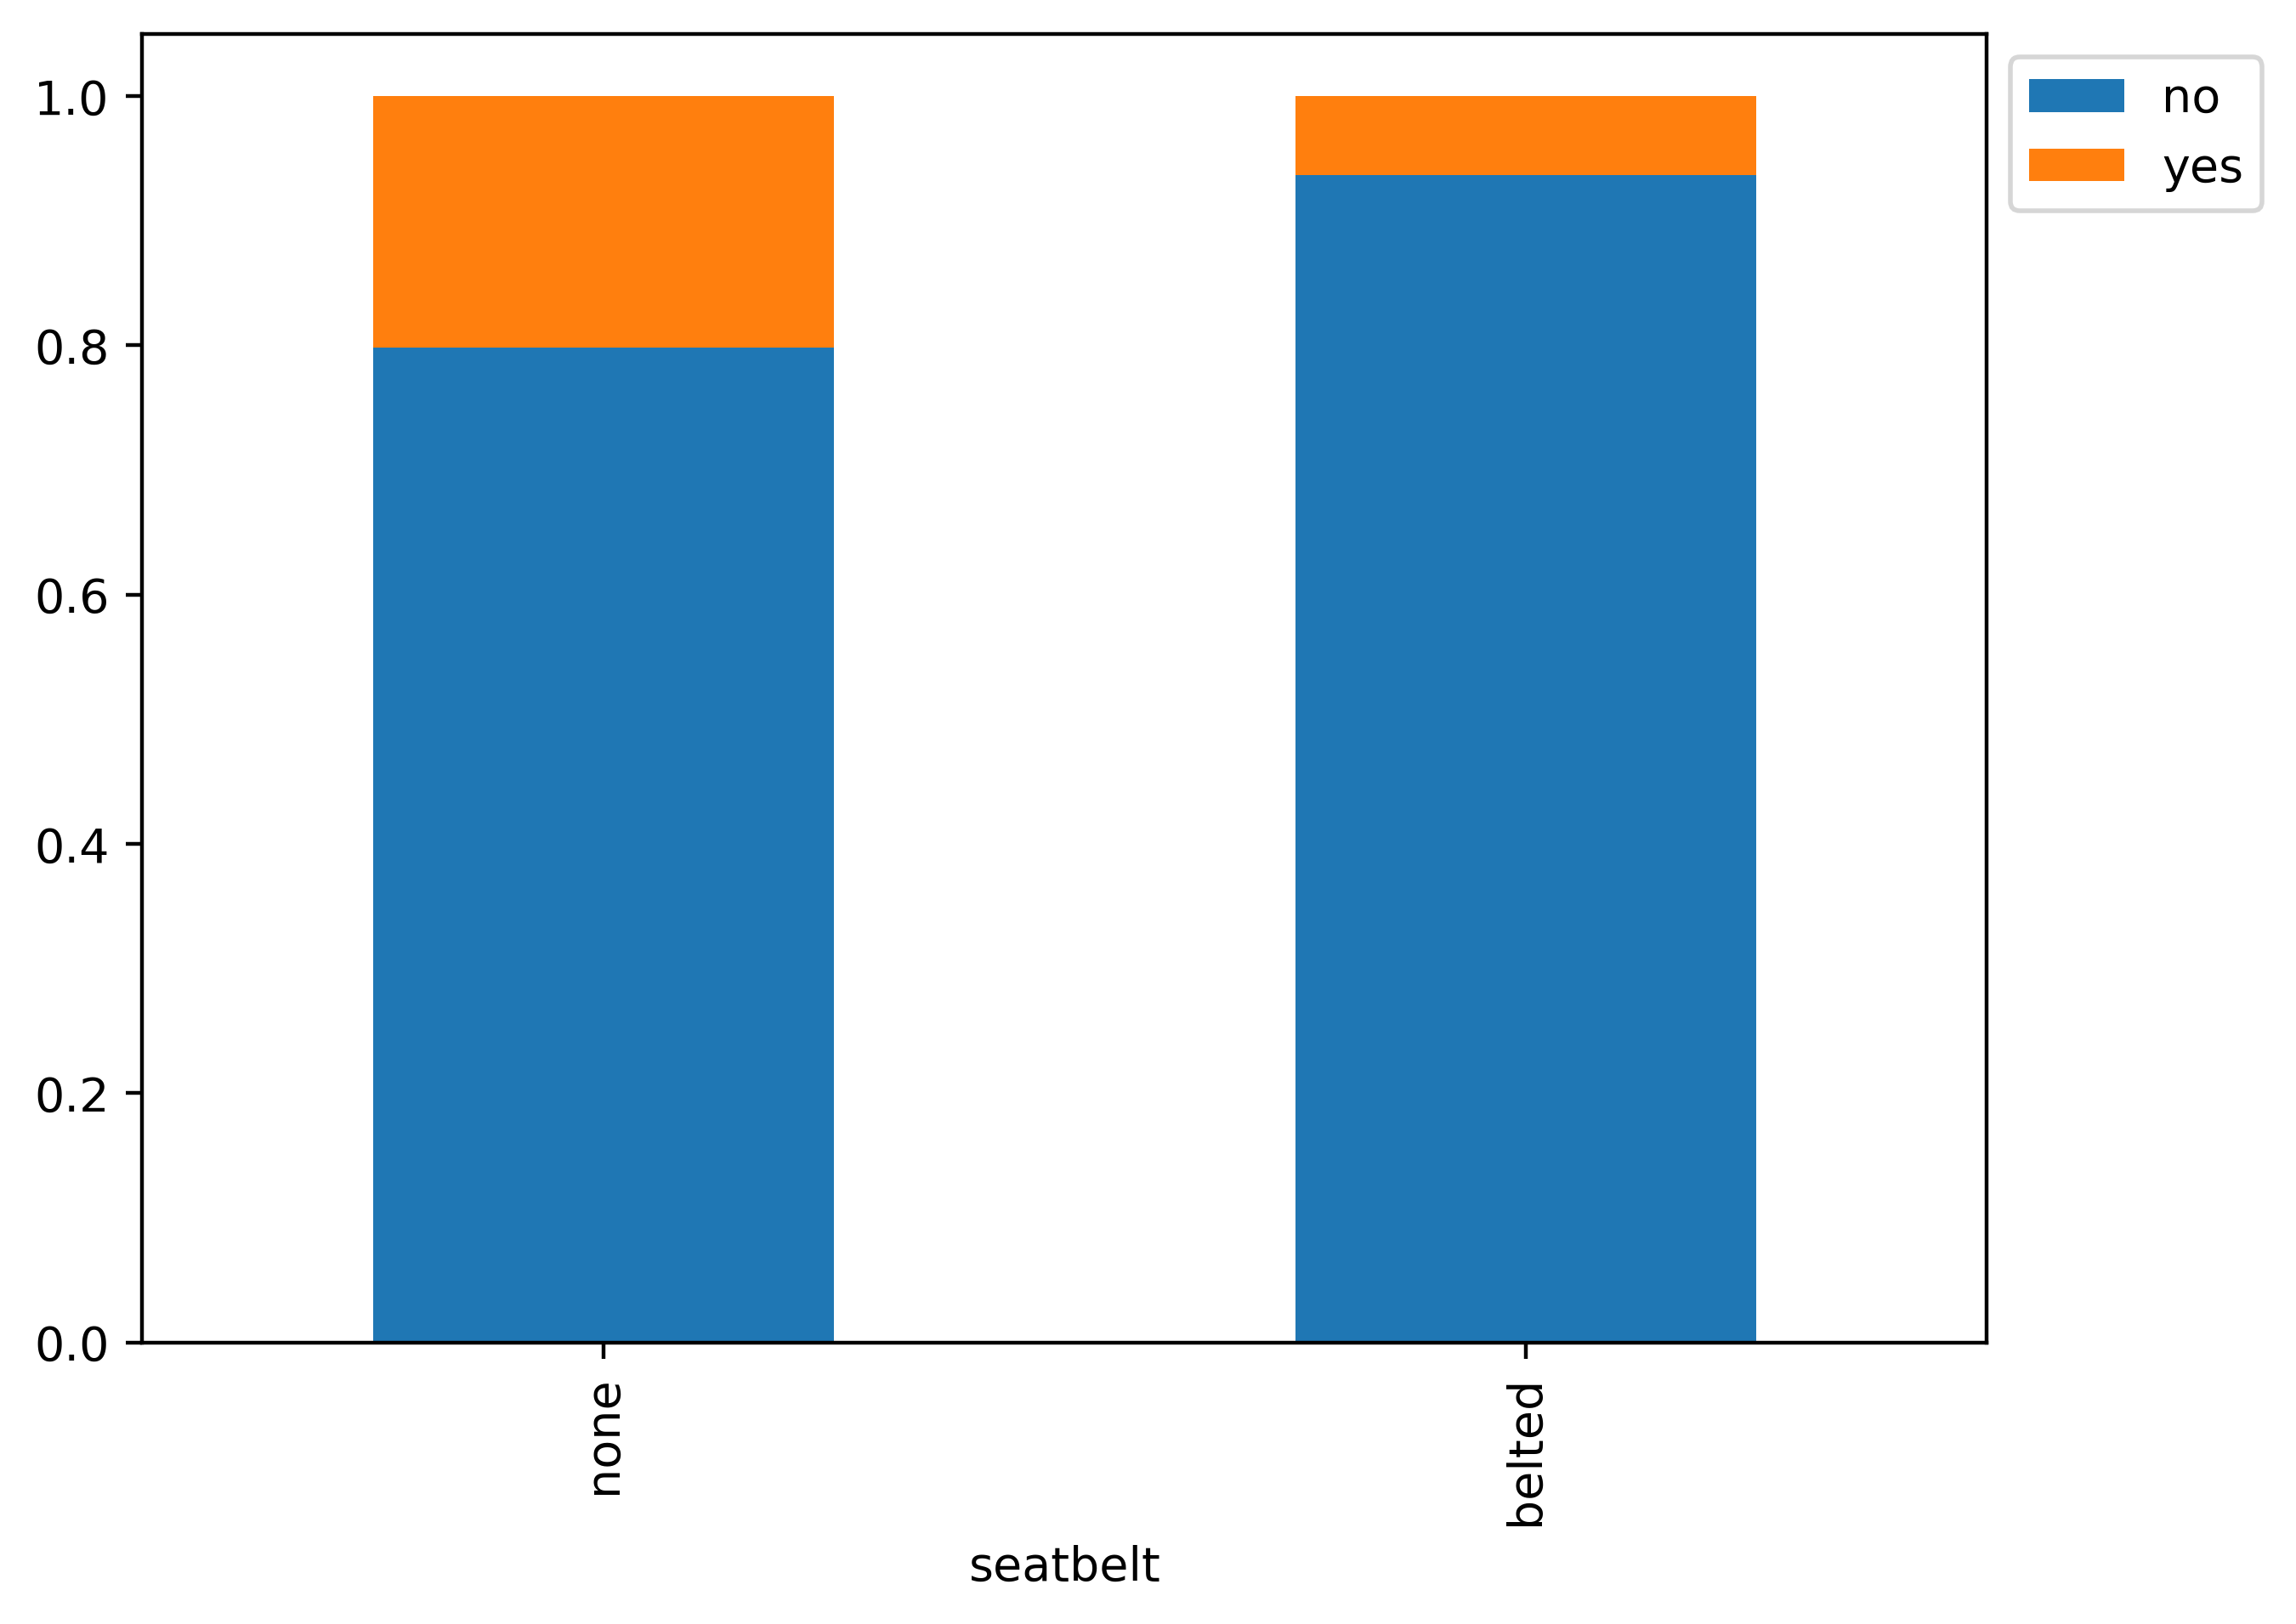
\includegraphics[width=\textwidth]{seat_belt_stack_deceased.png}
		\caption{}
		\label{fig:seat_belt_stack_deceased}
	\end{subfigure}
	\hfill
	\begin{subfigure}[t]{0.32\textwidth}
		\centering
		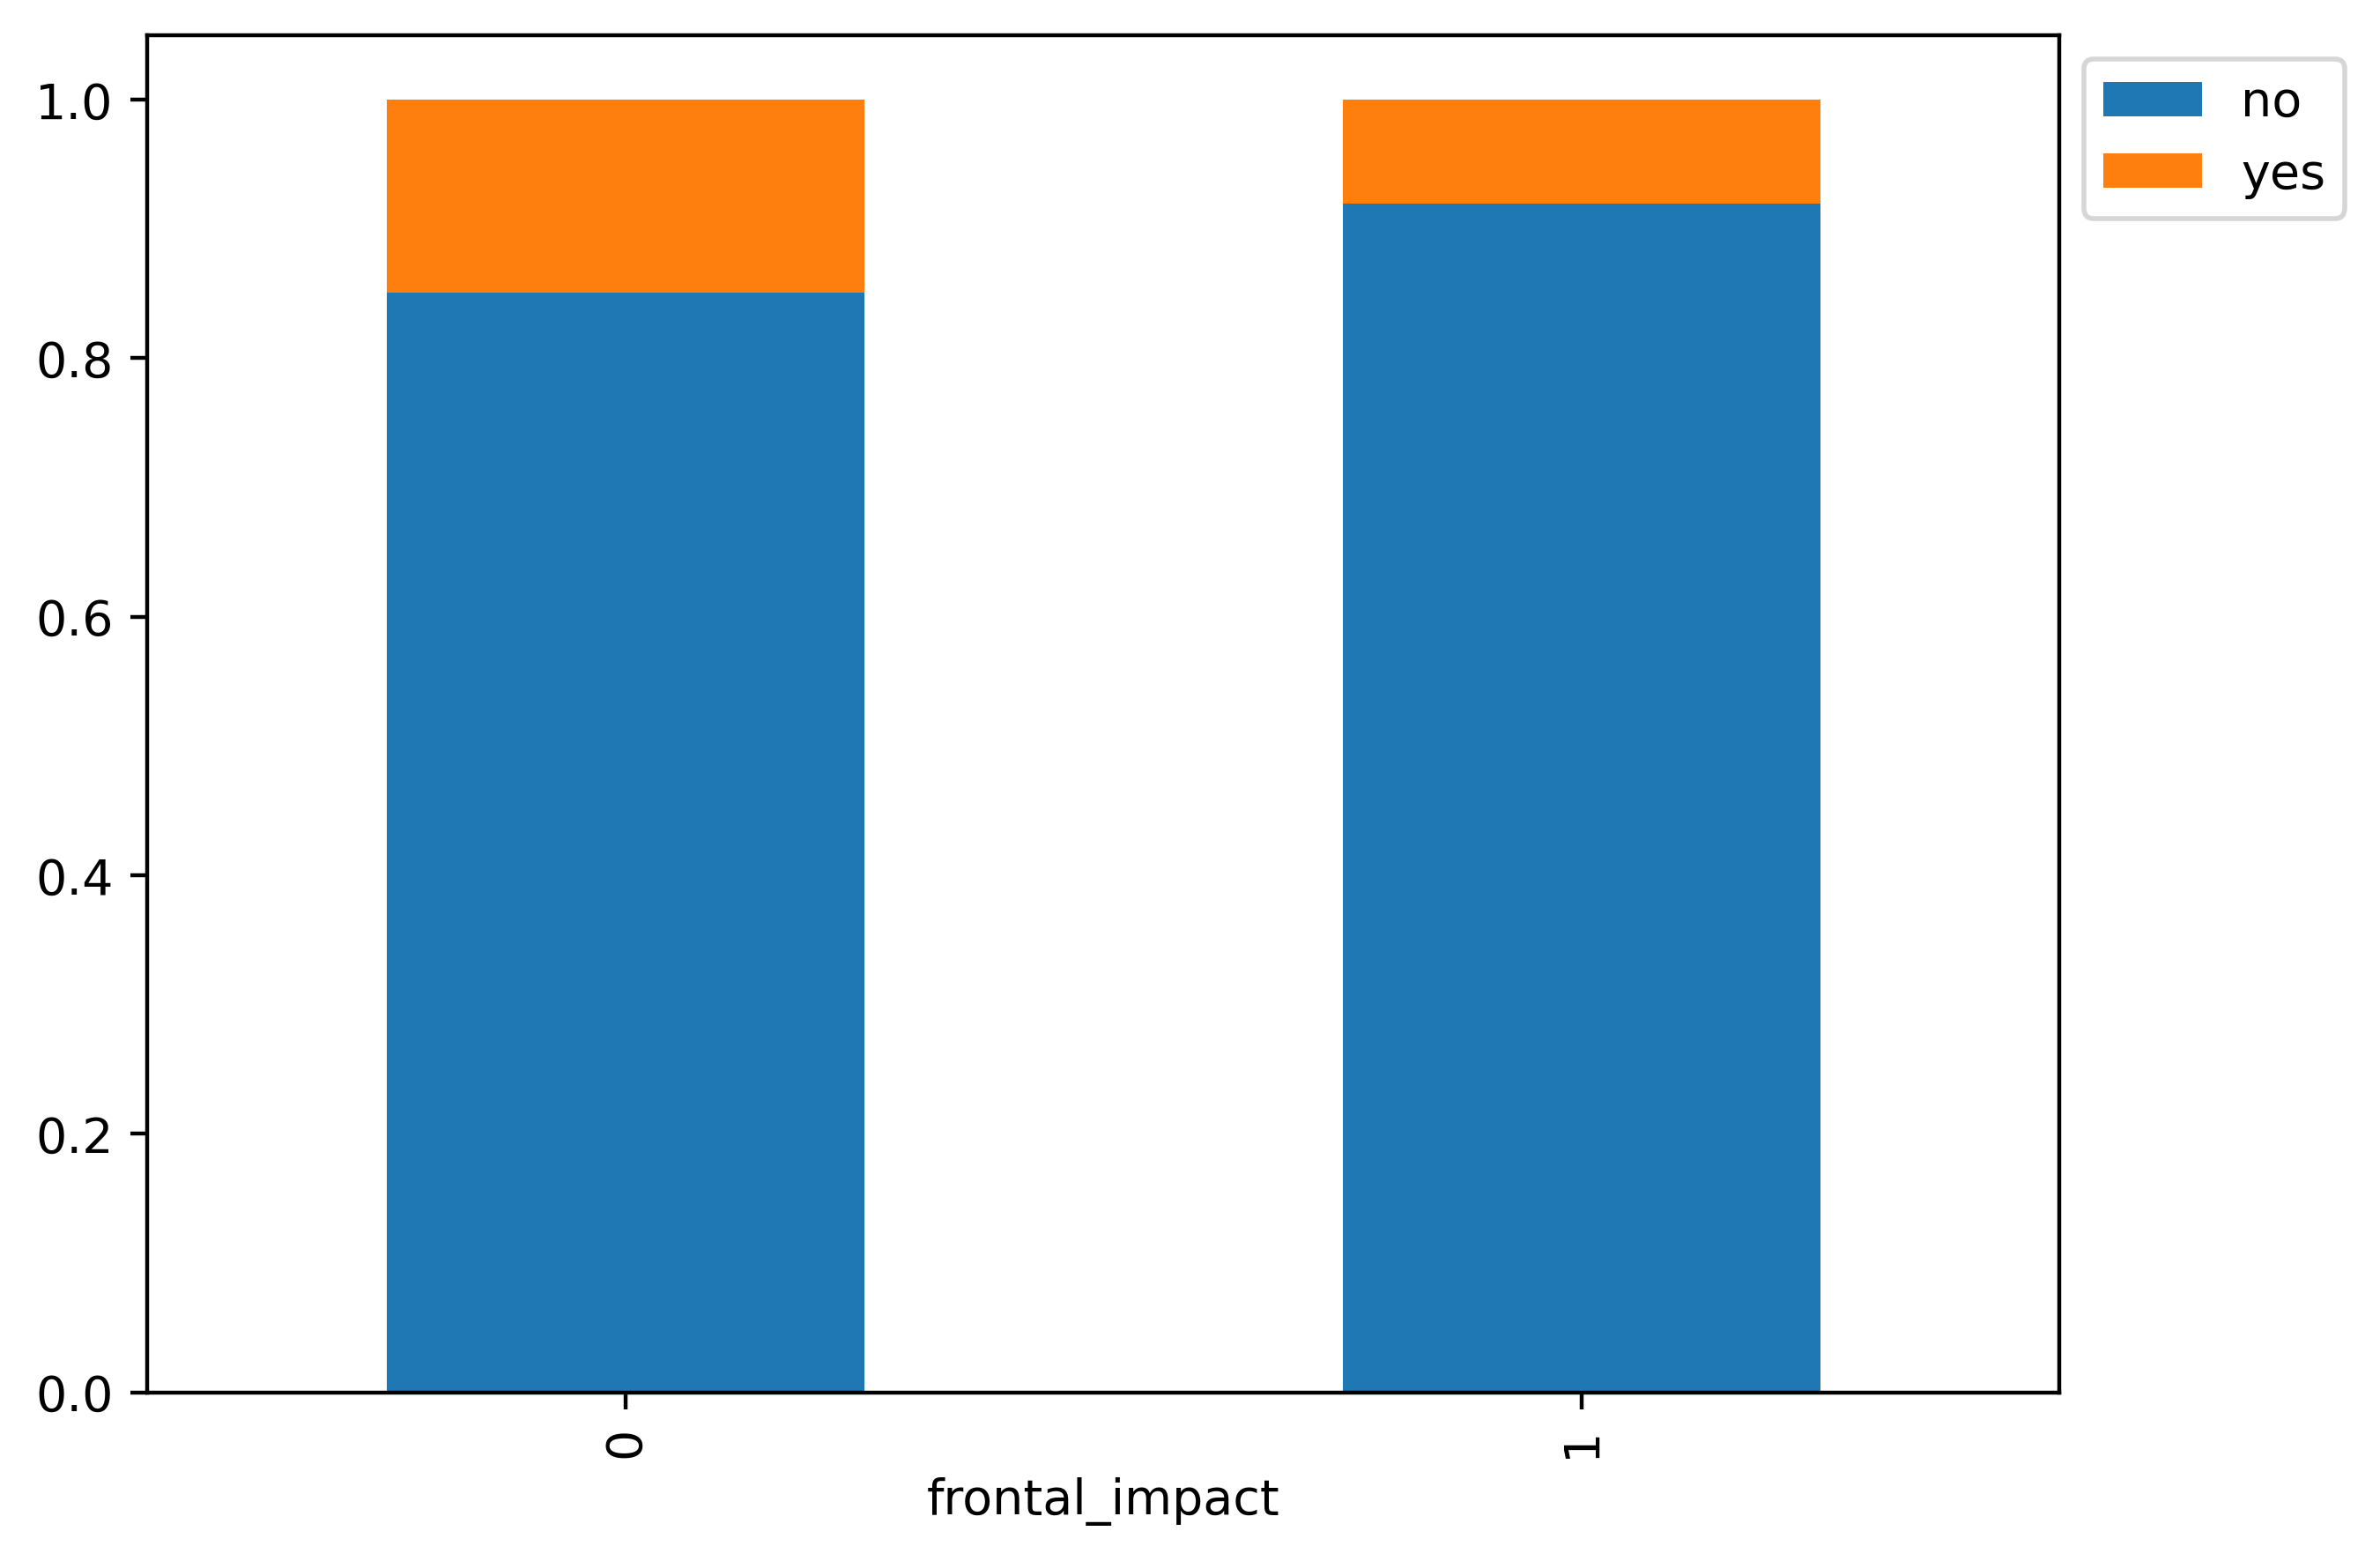
\includegraphics[width=\textwidth]{fontal_impact_stack_deceased.png}
		\caption{}
		\label{fig:fontal_impact_stack_deceased}
	\end{subfigure}
	\hfill
	\begin{subfigure}[t]{0.32\textwidth}
		\centering
		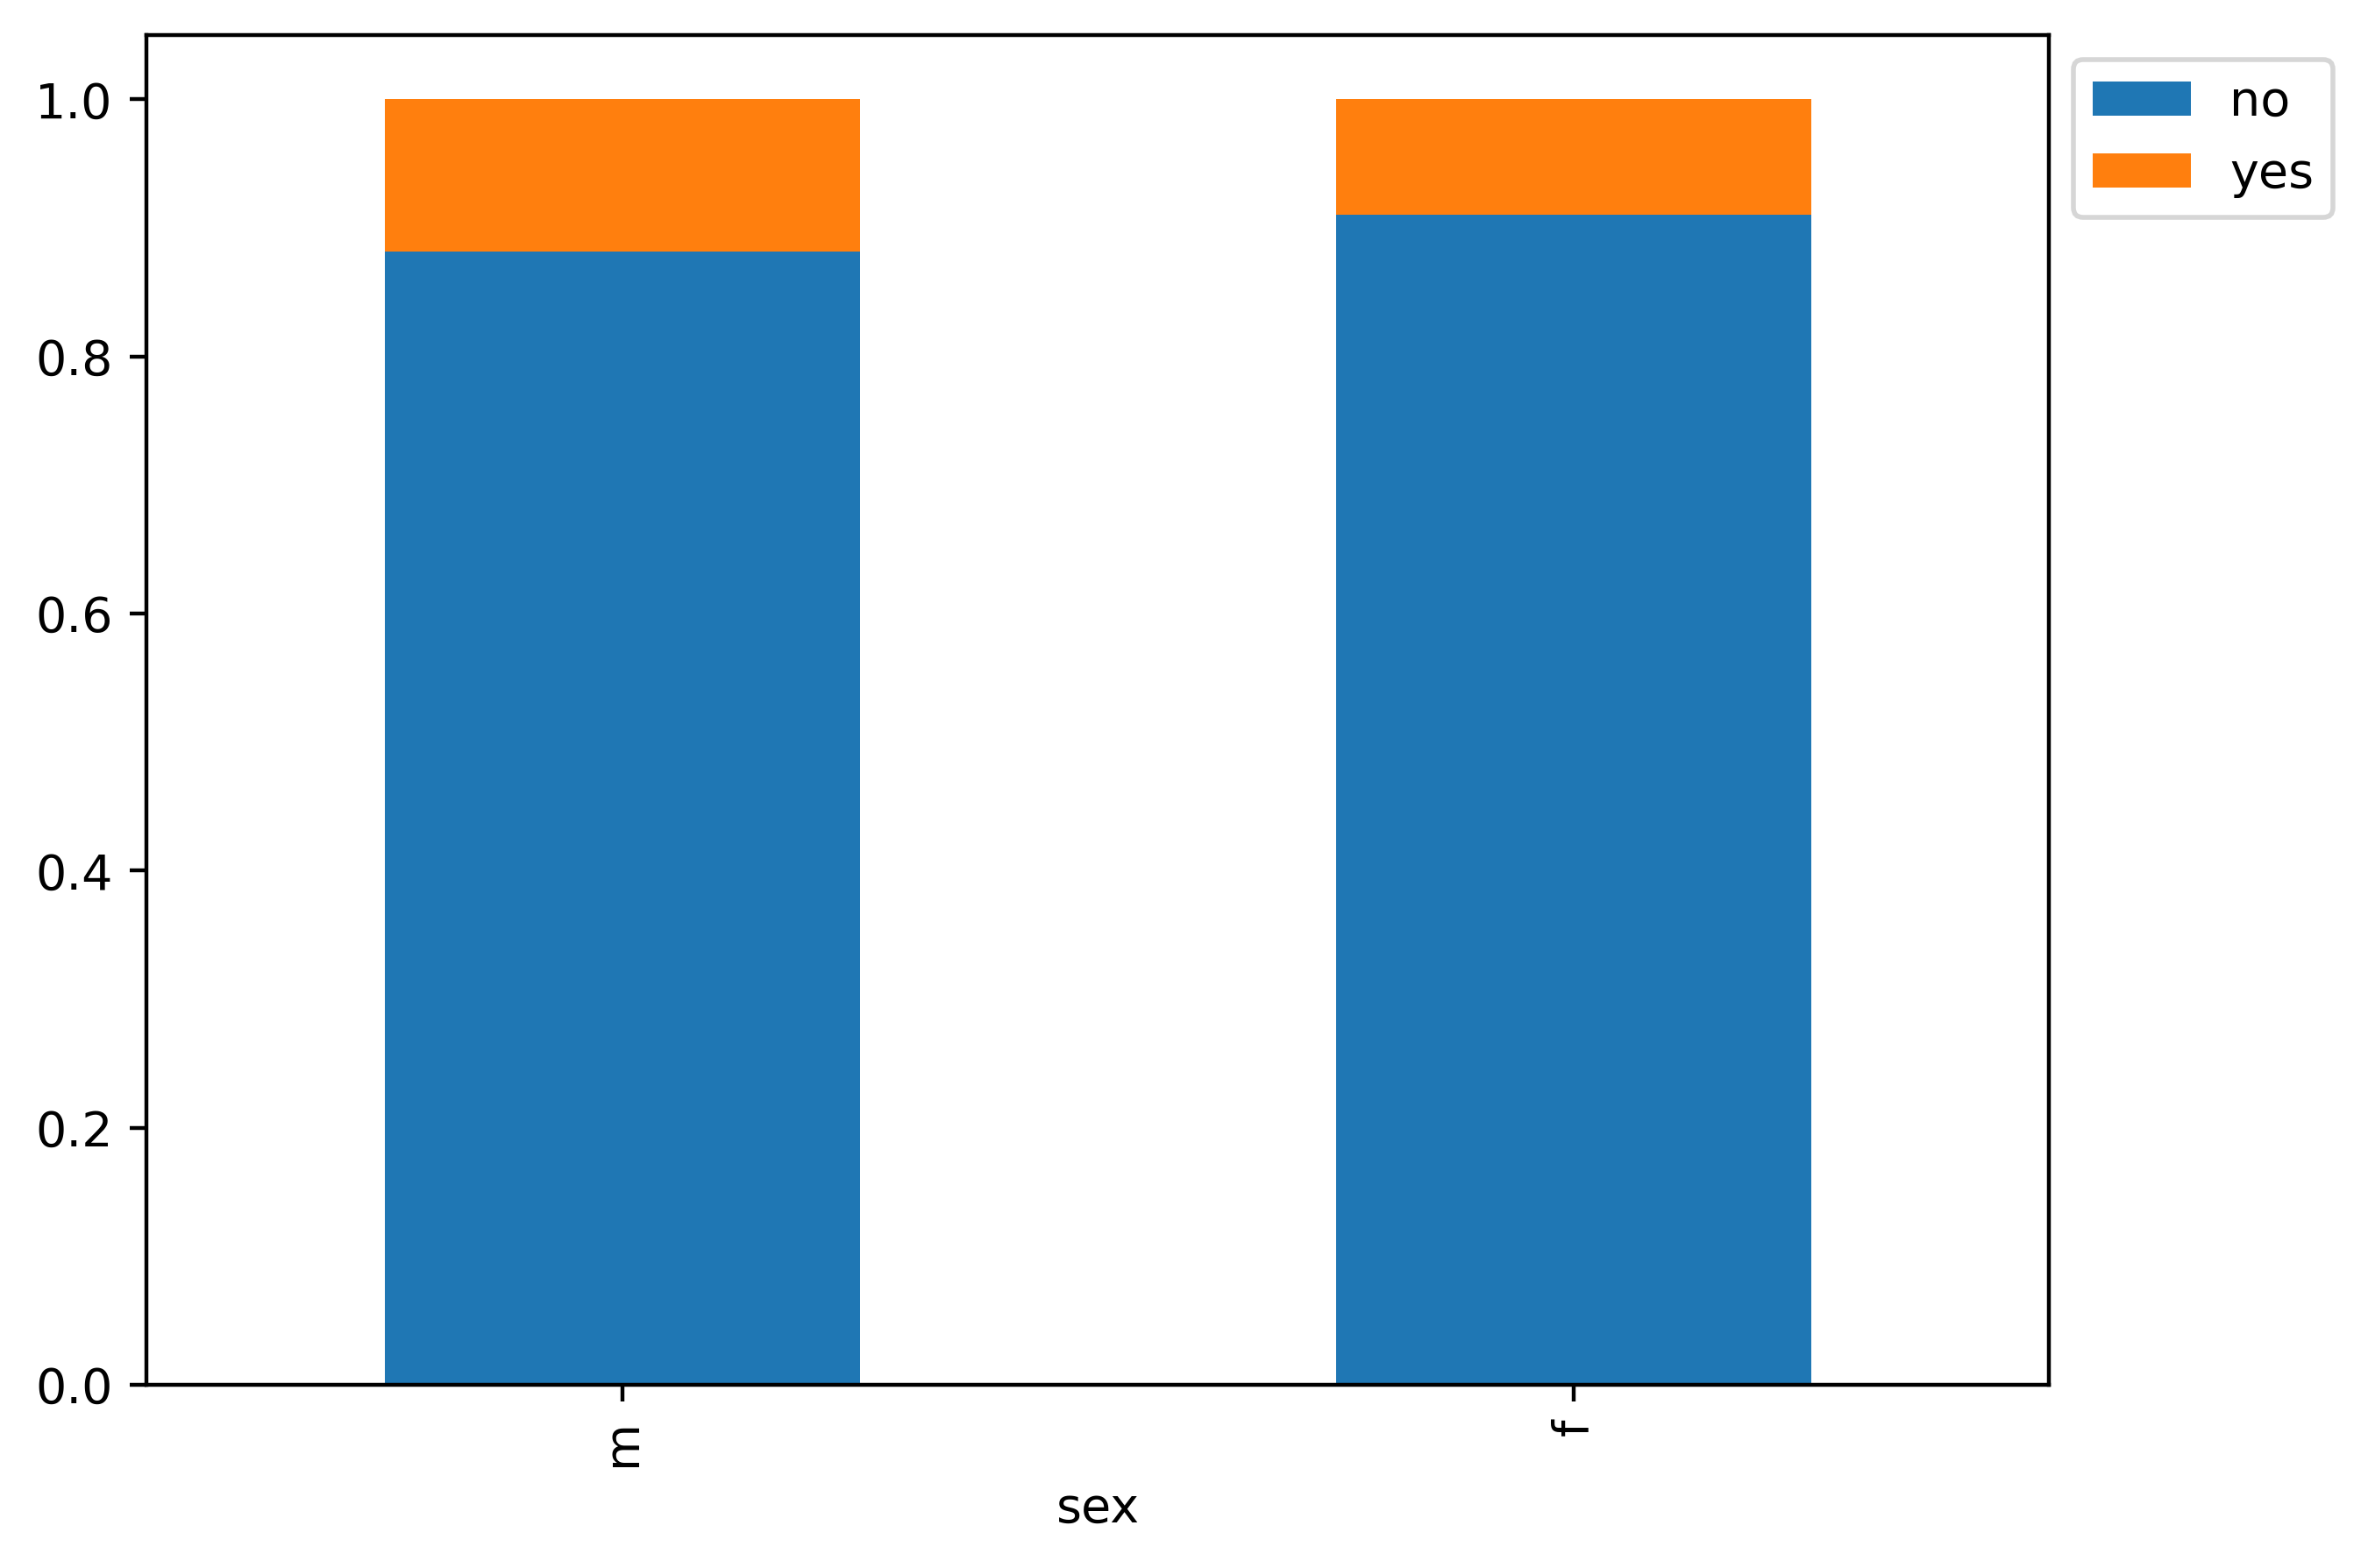
\includegraphics[width=\textwidth]{sex_stack_deceaed.png}
		\caption{}
		\label{fig:sex_stack_deceaed}
	\end{subfigure}
	\hfill
	\begin{subfigure}[t]{0.32\textwidth}
		\centering
		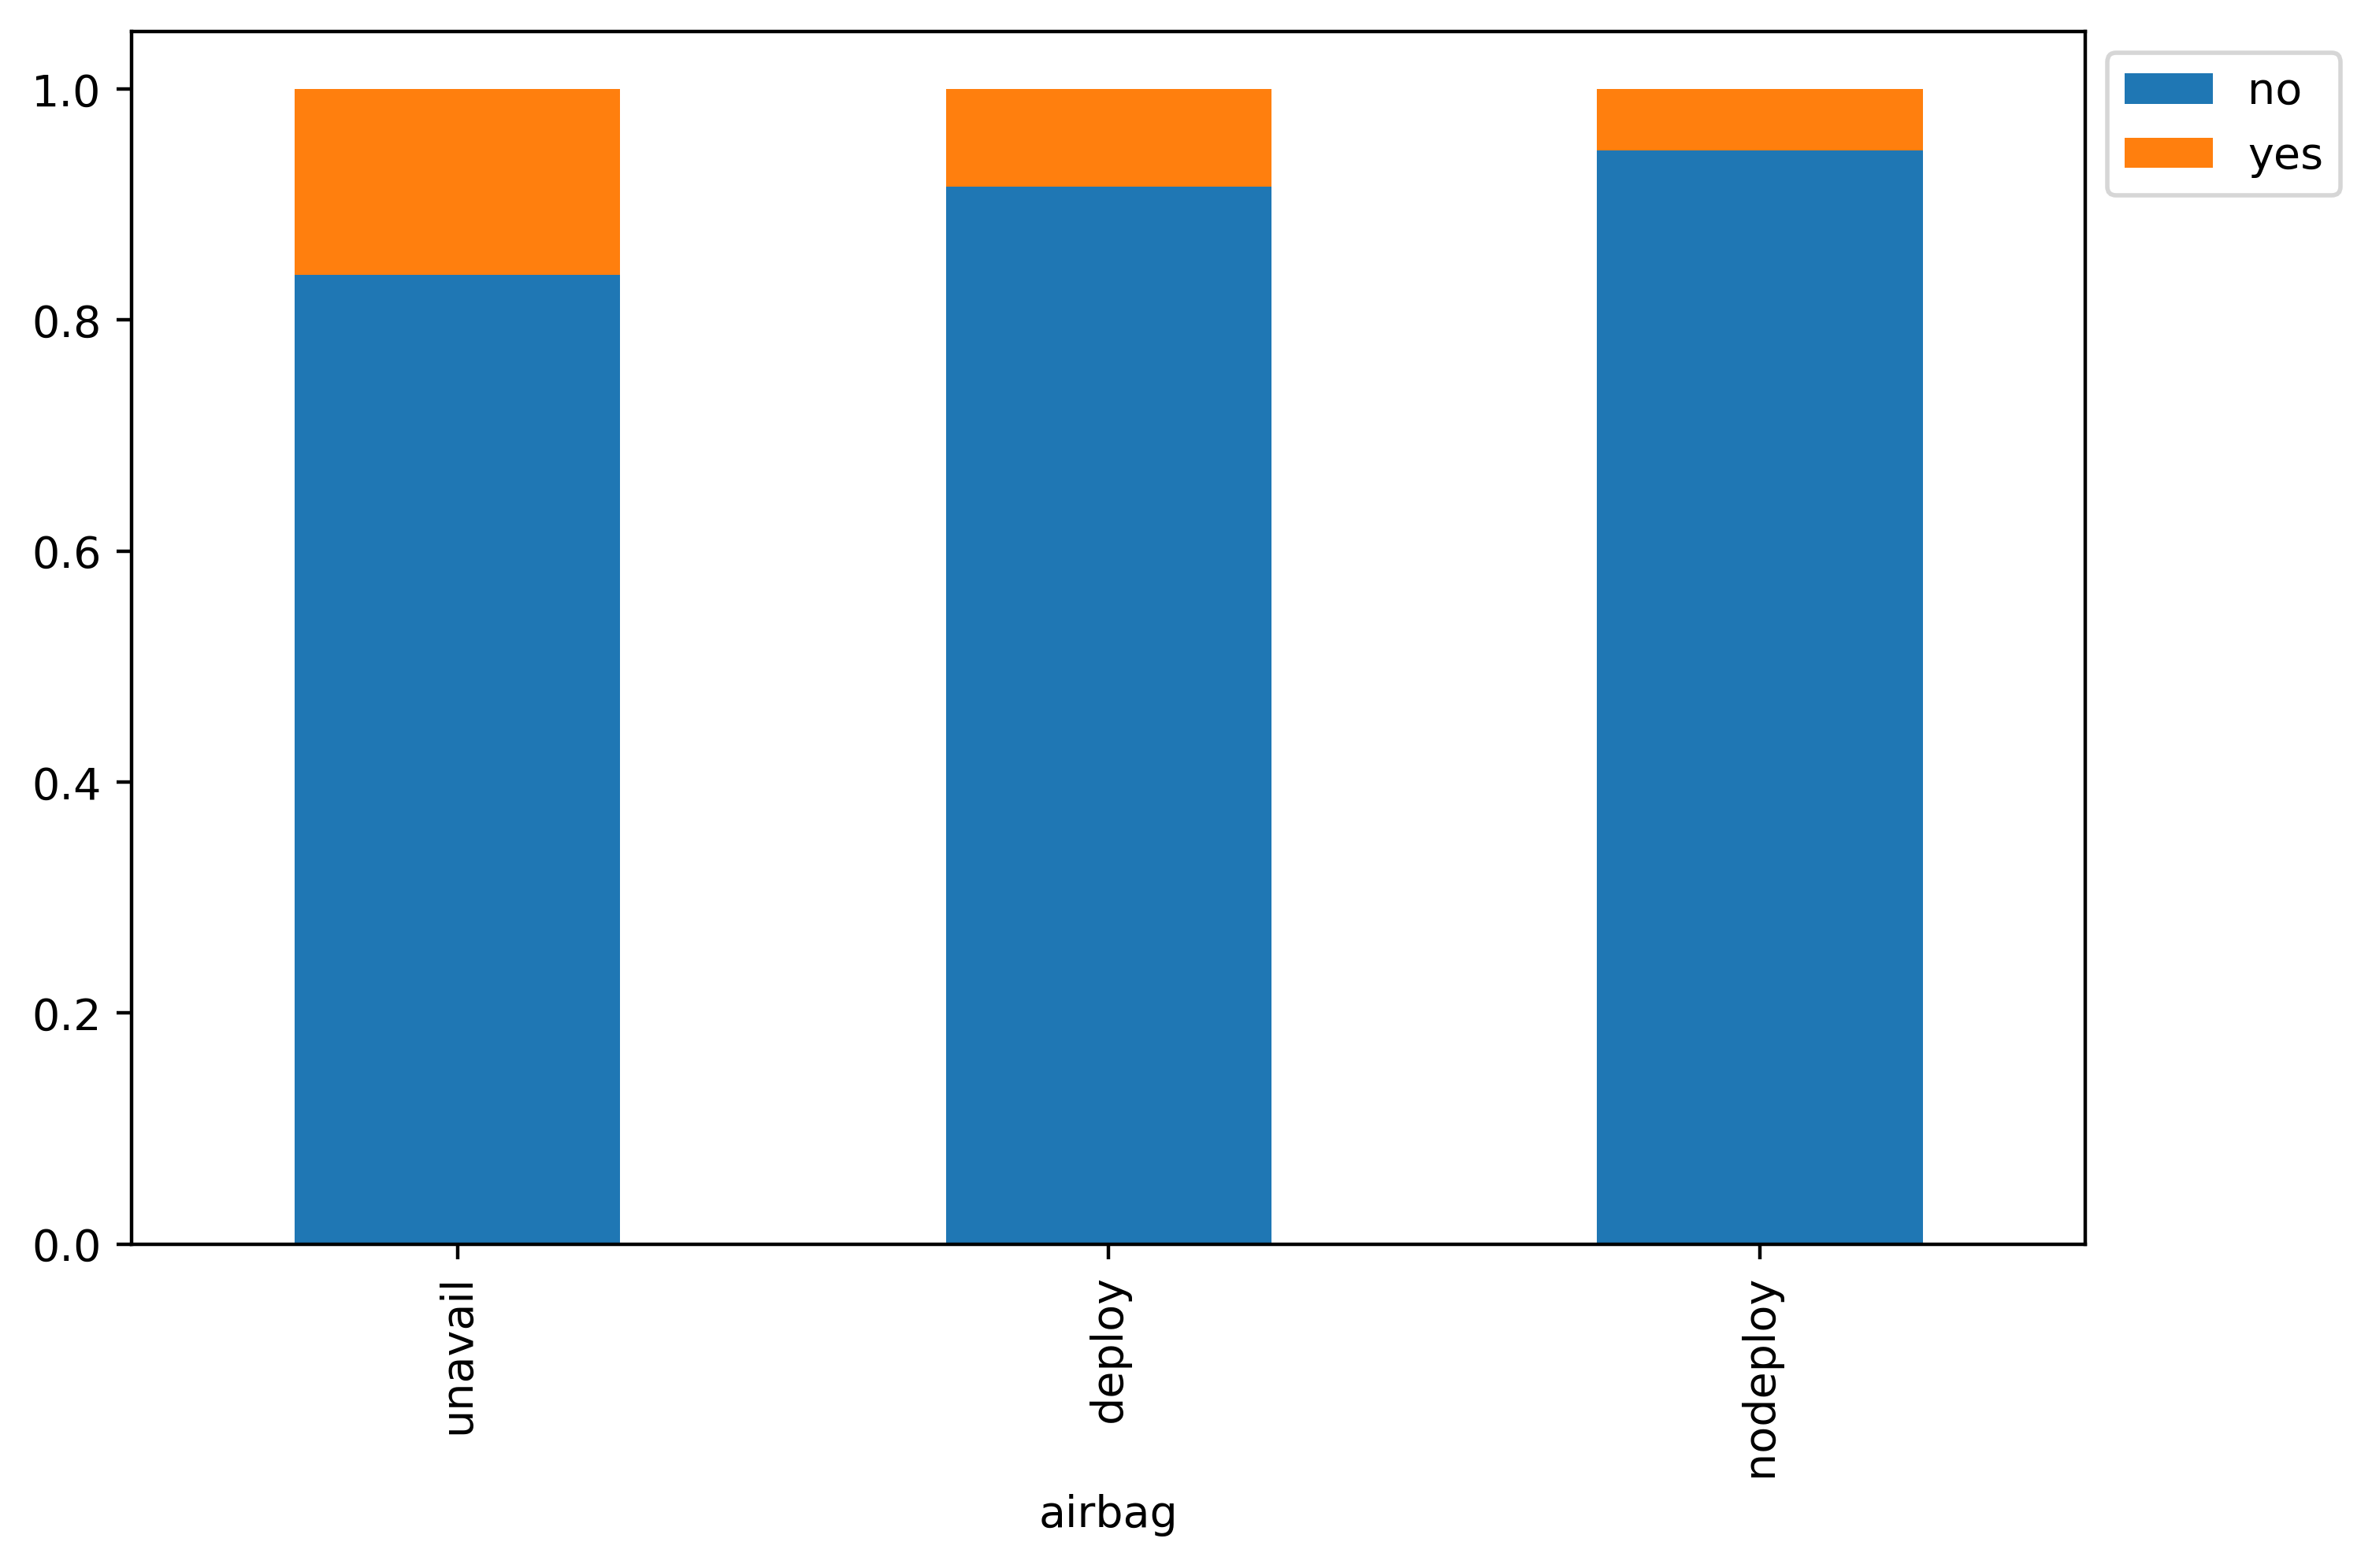
\includegraphics[width=\textwidth]{airbag_stack_deceased.png}
		\caption{}
		\label{fig:airbag_stack_deceased}
	\end{subfigure}
	\hfill
	\begin{subfigure}[t]{0.33\textwidth}
		\centering
		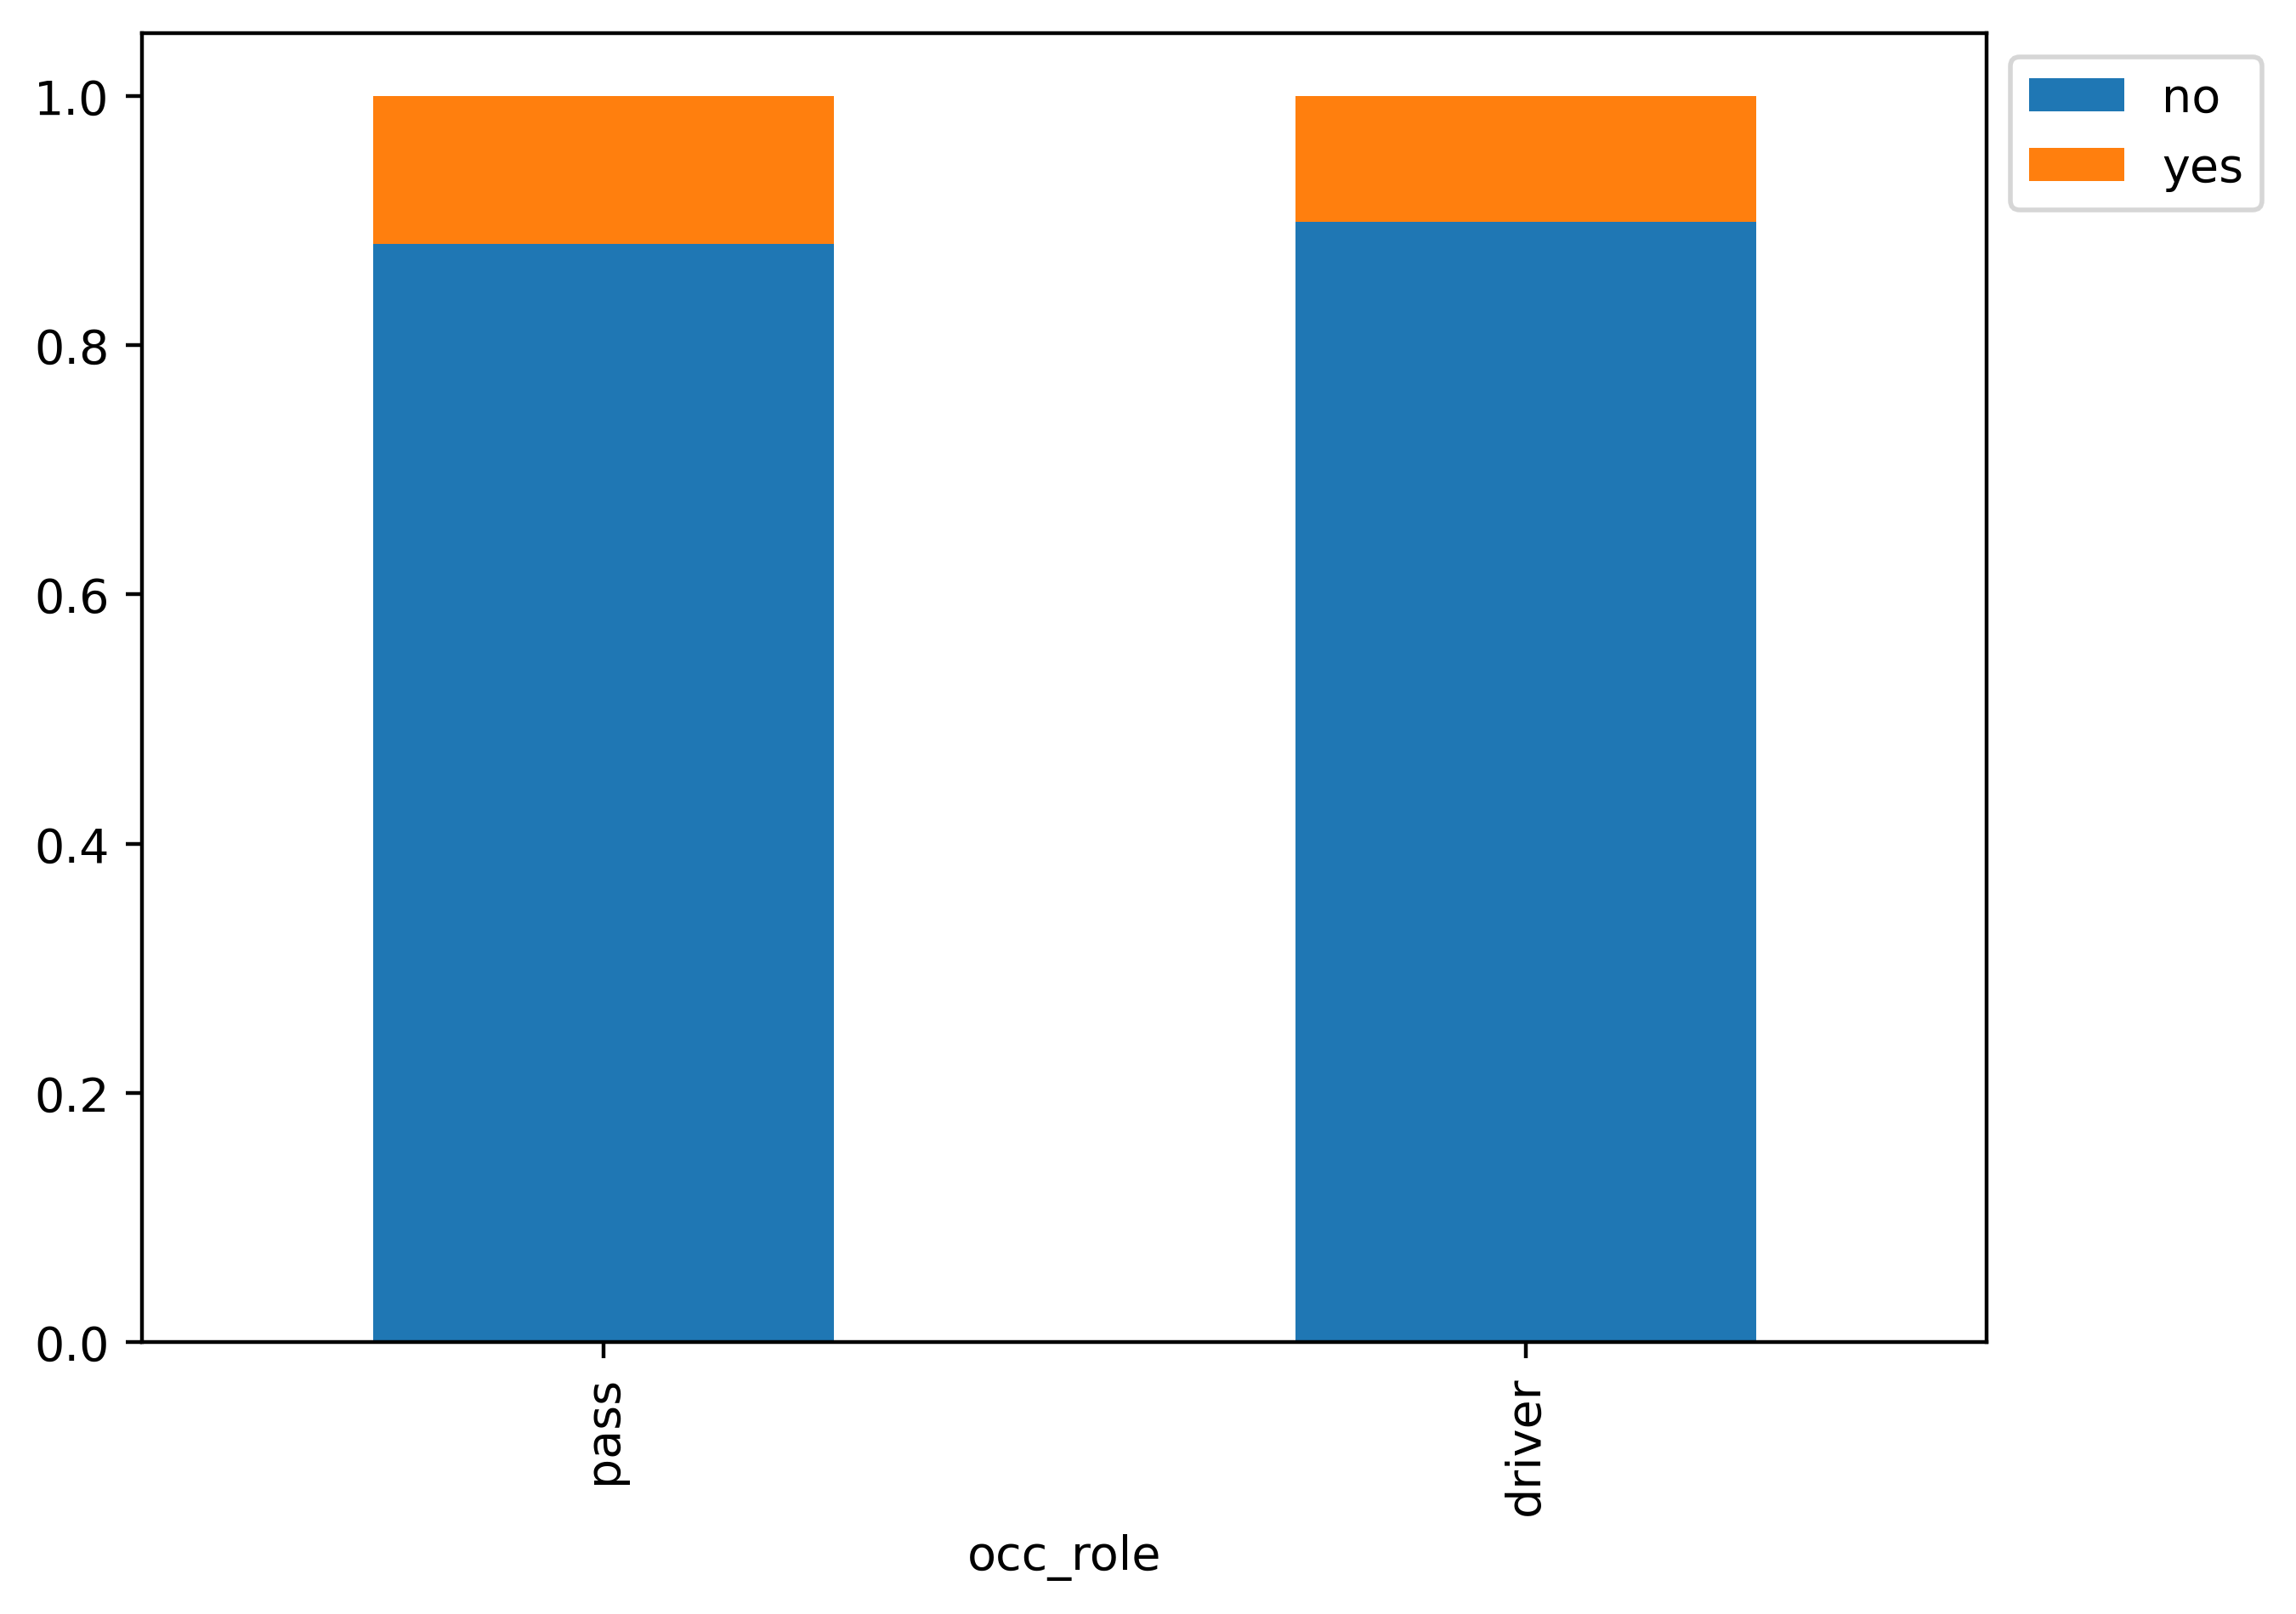
\includegraphics[width=\textwidth]{occ_role_stack_deceased.png}
		\caption{}
		\label{fig:occ_role_stack_deceased}
	\end{subfigure}
		\caption{Stack plot distribution of categorical variables with respect target.}
		\label{fig:stackplot_wrt_target}
	\end{figure}
Figure \ref{fig:stackplot_wrt_target} shows stack plot of categorical variables with respect to target(deceased). The stack plot for speed range \ref{fig:speed_range_stack_deceased} shows the distribution of deceased individuals across different speed ranges at the time of the crash. Higher speeds typically correlate with a higher number of fatalities, indicating the critical impact of speed on crash severity.

The plot on \ref{fig:seat_belt_stack_deceased} illustrates the relationship between seat belt usage and fatalities. It shows a higher proportion of deceased individuals not wearing seat belts, emphasizing the importance of seat belt usage in reducing fatalities.
 
The stack plot for frontal impact \ref{fig:fontal_impact_stack_deceased} highlights the distribution of fatalities in crashes involving frontal impacts. Frontal impacts are often more severe, leading to a higher number of fatalities compared to other types of impacts.

The plot on figure \ref{fig:sex_stack_deceaed} shows the distribution of deceased individuals by sex. It reveals that there is a slight difference in fatalities between males and females(males have slightly more fatalities), which could be due to various factors such as driving behavior or exposure risk etc.

The stack plot for airbag deployment on figure \ref{fig:airbag_stack_deceased} indicates the effectiveness of airbags in preventing fatalities. A lower proportion of deceased individuals in crashes where airbags deployed successfully would suggest their crucial role in saving lives.

The plot on figure \ref{fig:occ_role_stack_deceased} shows the distribution of fatalities based on the role of the occupant (e.g., driver, front passenger, rear passenger). It helps identify which positions in the vehicle are more vulnerable during crashes. As per this plot we find that passengers are more prone to severity than drivers most likely because passenger seats are usually not equipped with high efficient airbags compared to front driver seats.
	\begin{figure}[h]
		\centering
		\begin{subfigure}[t]{0.495\linewidth}
			\centering
			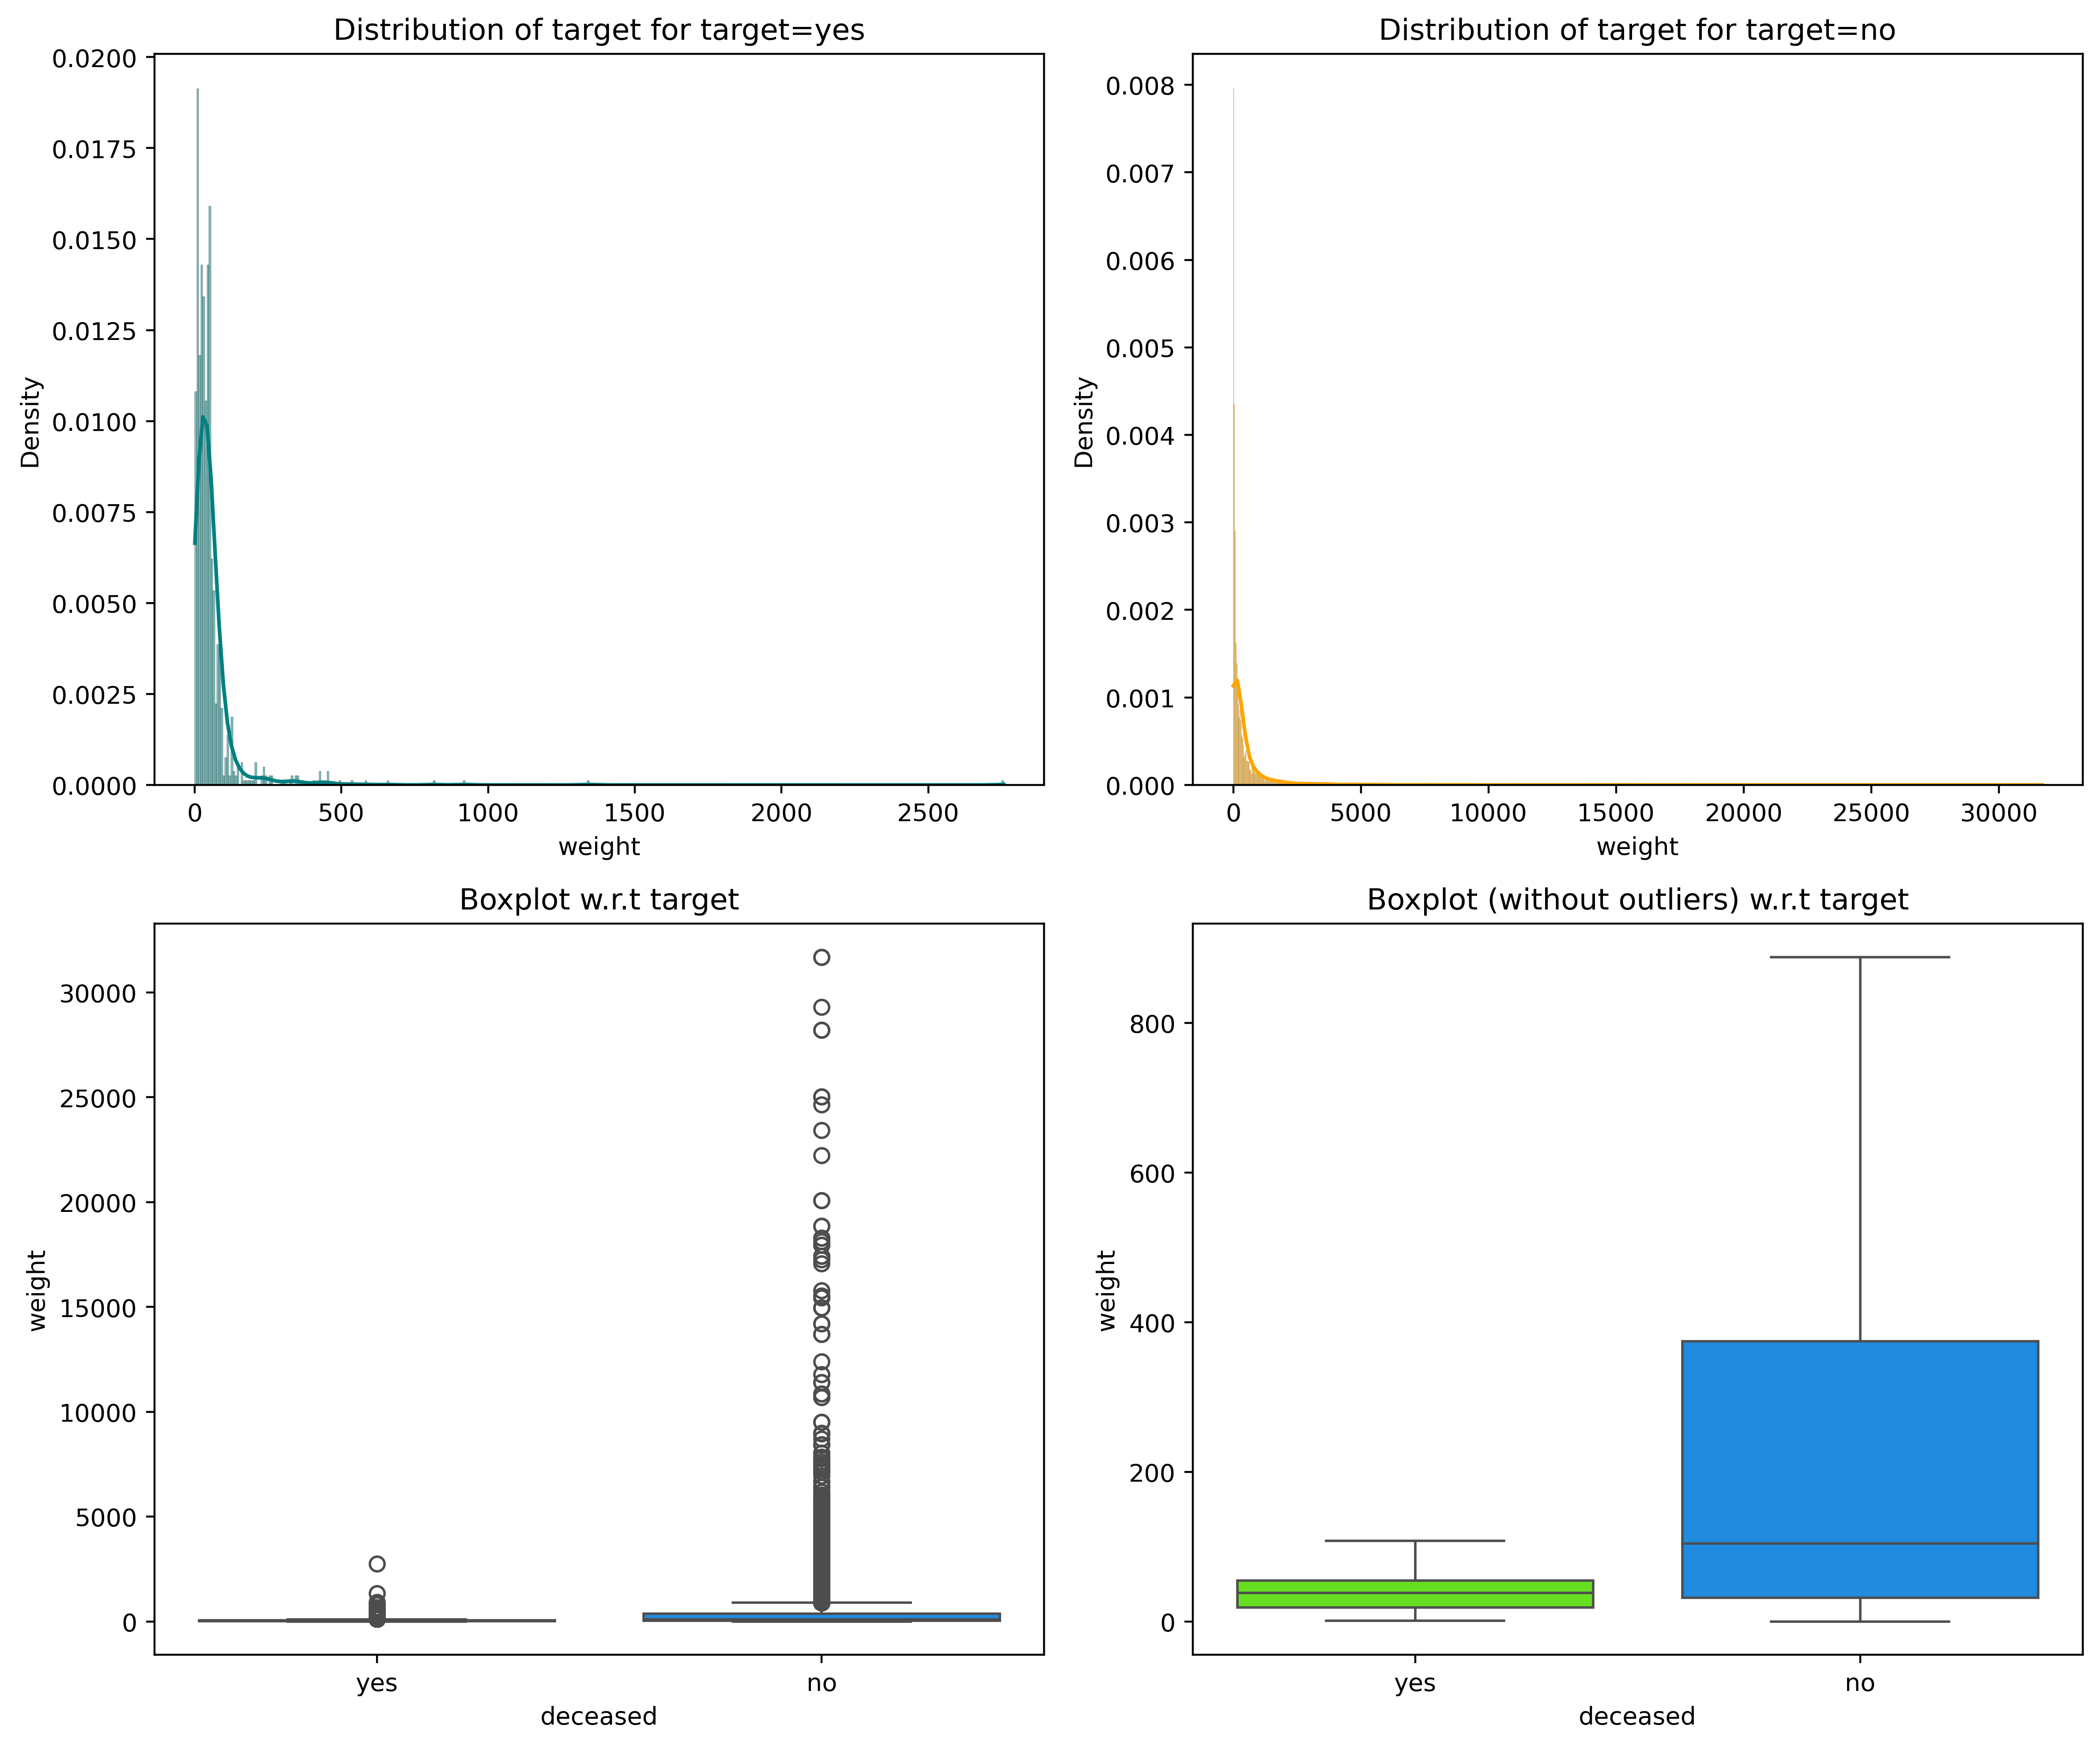
\includegraphics[width=\linewidth]{weight_target.png}
			\caption{Boxplot of deceased with respect to weight factor.}
			\label{fig:weight_factor}
		\end{subfigure}
		\hfill
		\begin{subfigure}[t]{0.495\linewidth}
			\centering
			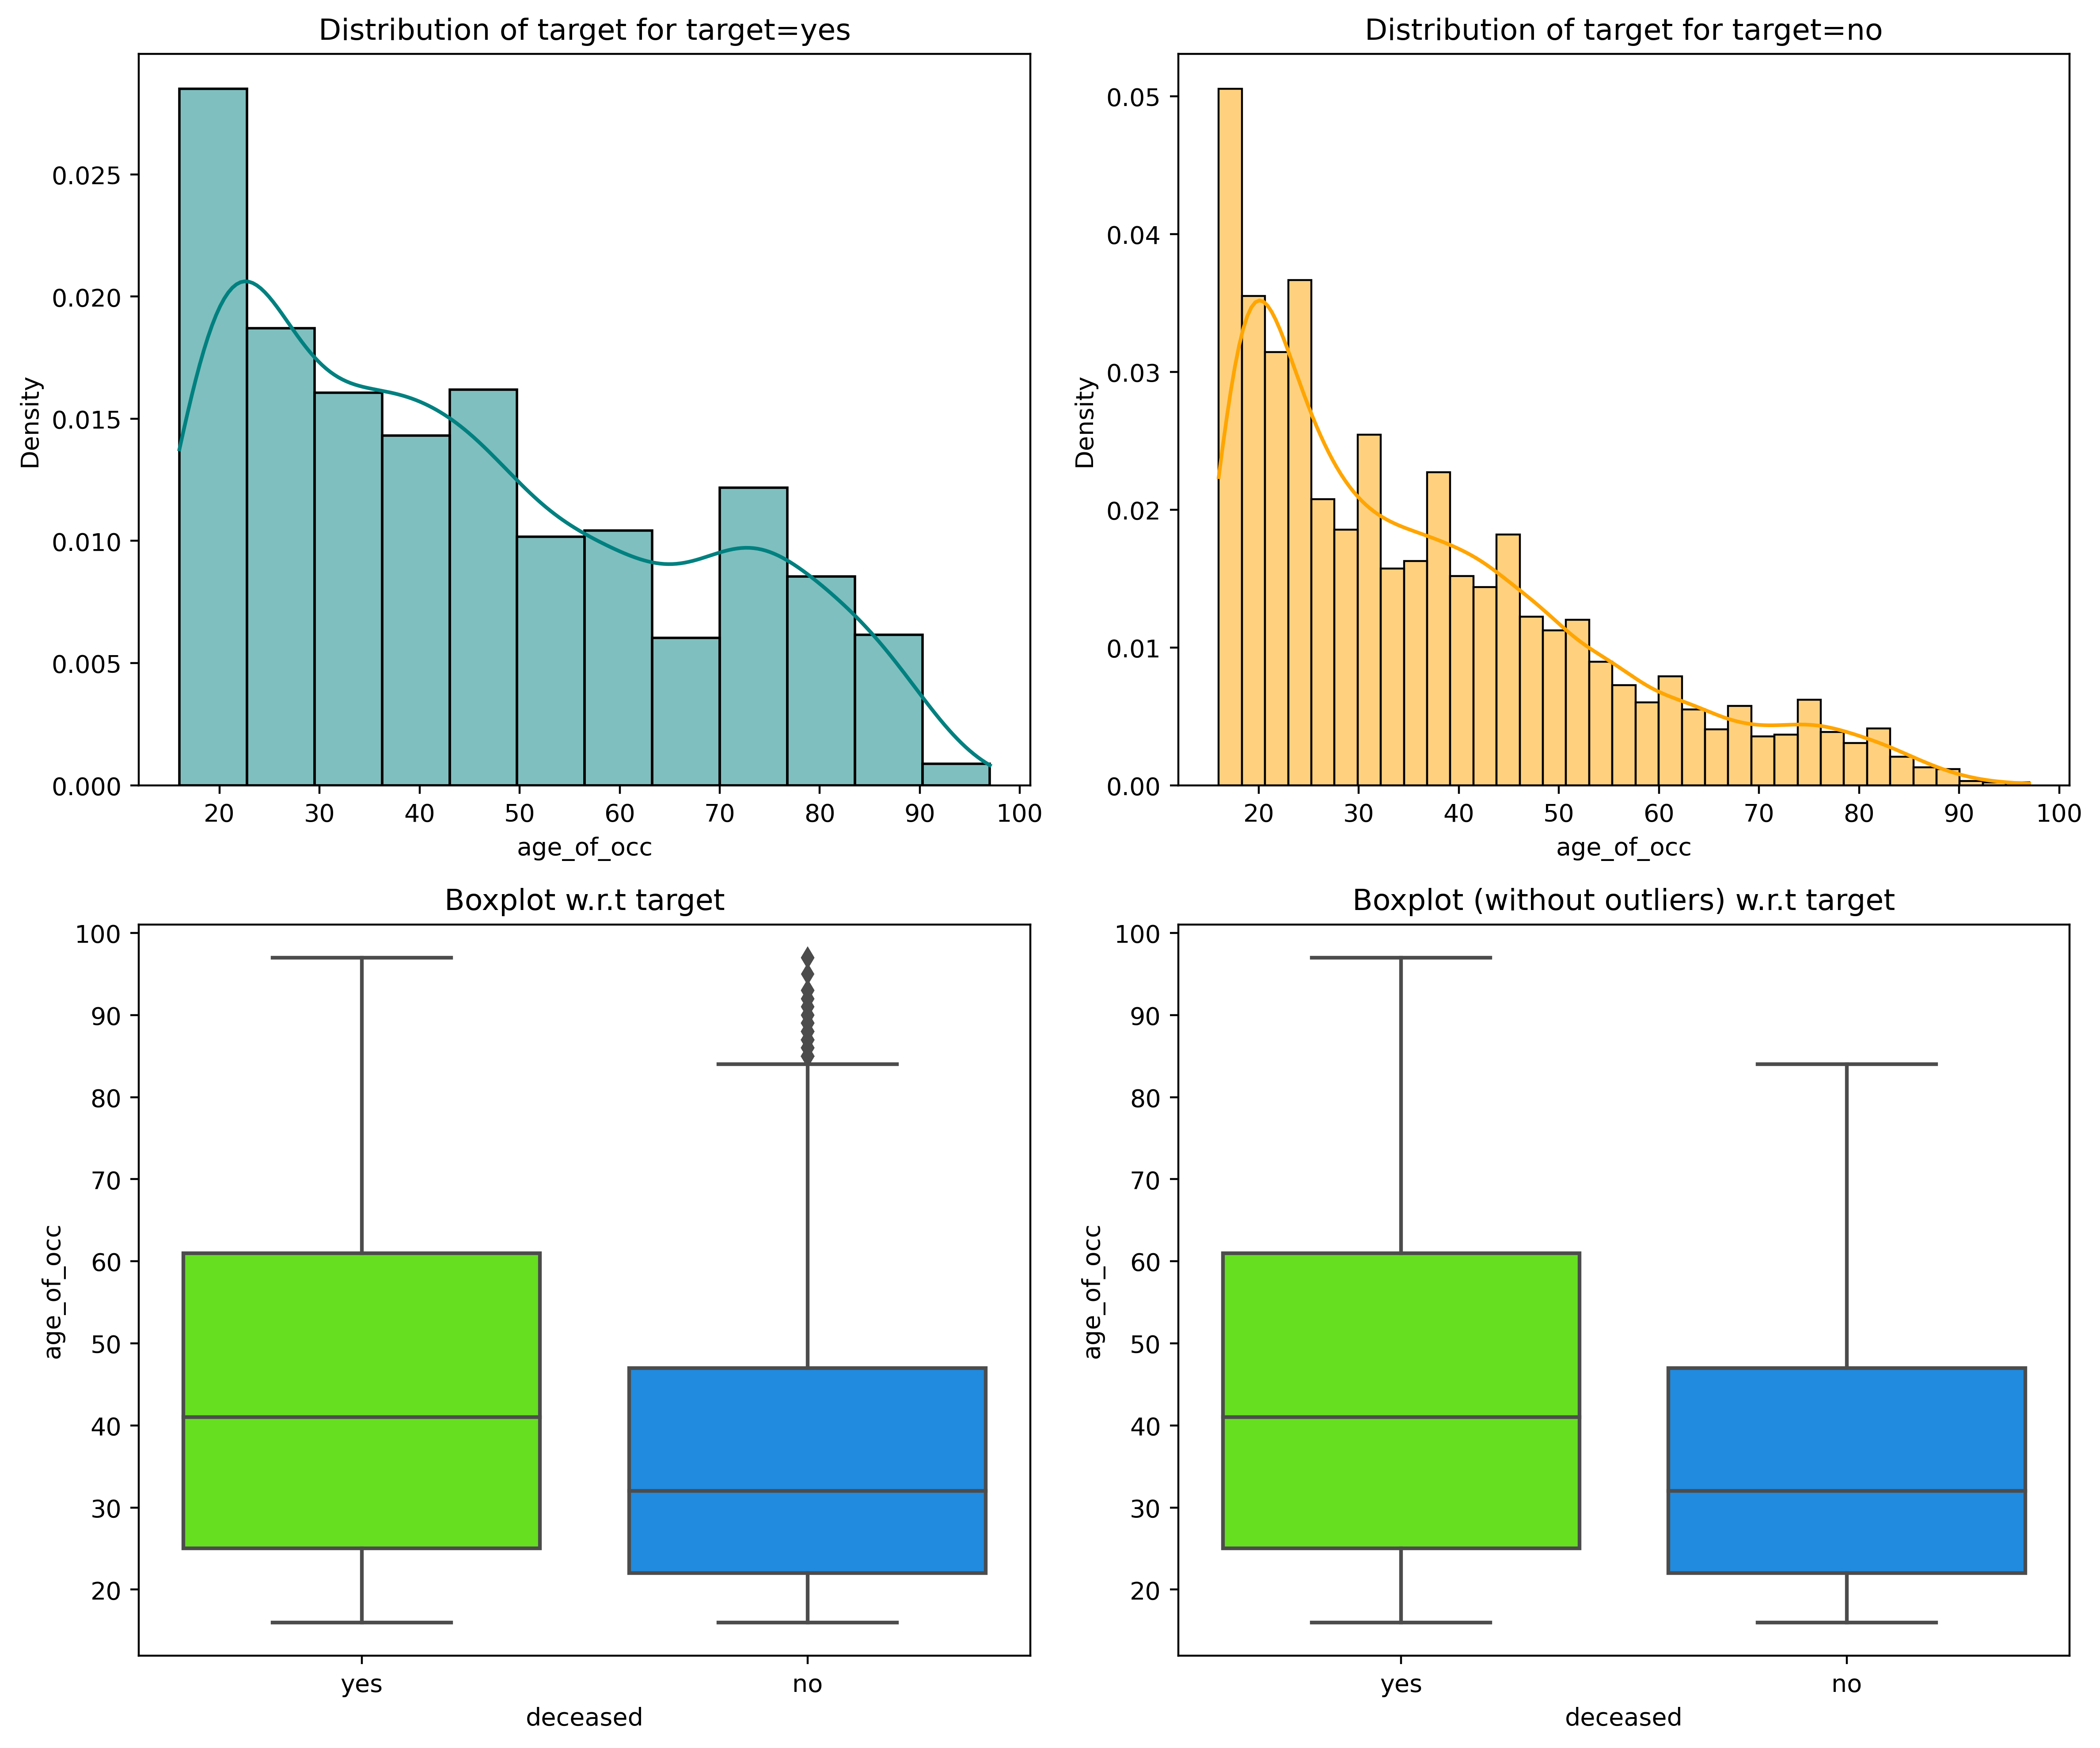
\includegraphics[width=\linewidth]{age_of_occ_wrt_target.png}
			\caption{Boxplot of deceased with respect to person's age}
			\label{fig:age_factor}
		\end{subfigure}
		\caption{Distribution showing role of age and weight factor in deceased cases.}
		\label{fig:Distribution showing role of age and weight factor in deceased cases. }
	\end{figure}
	\begin{figure}[h]
		\centering
		\begin{subfigure}[t]{0.495\linewidth}
			\centering
			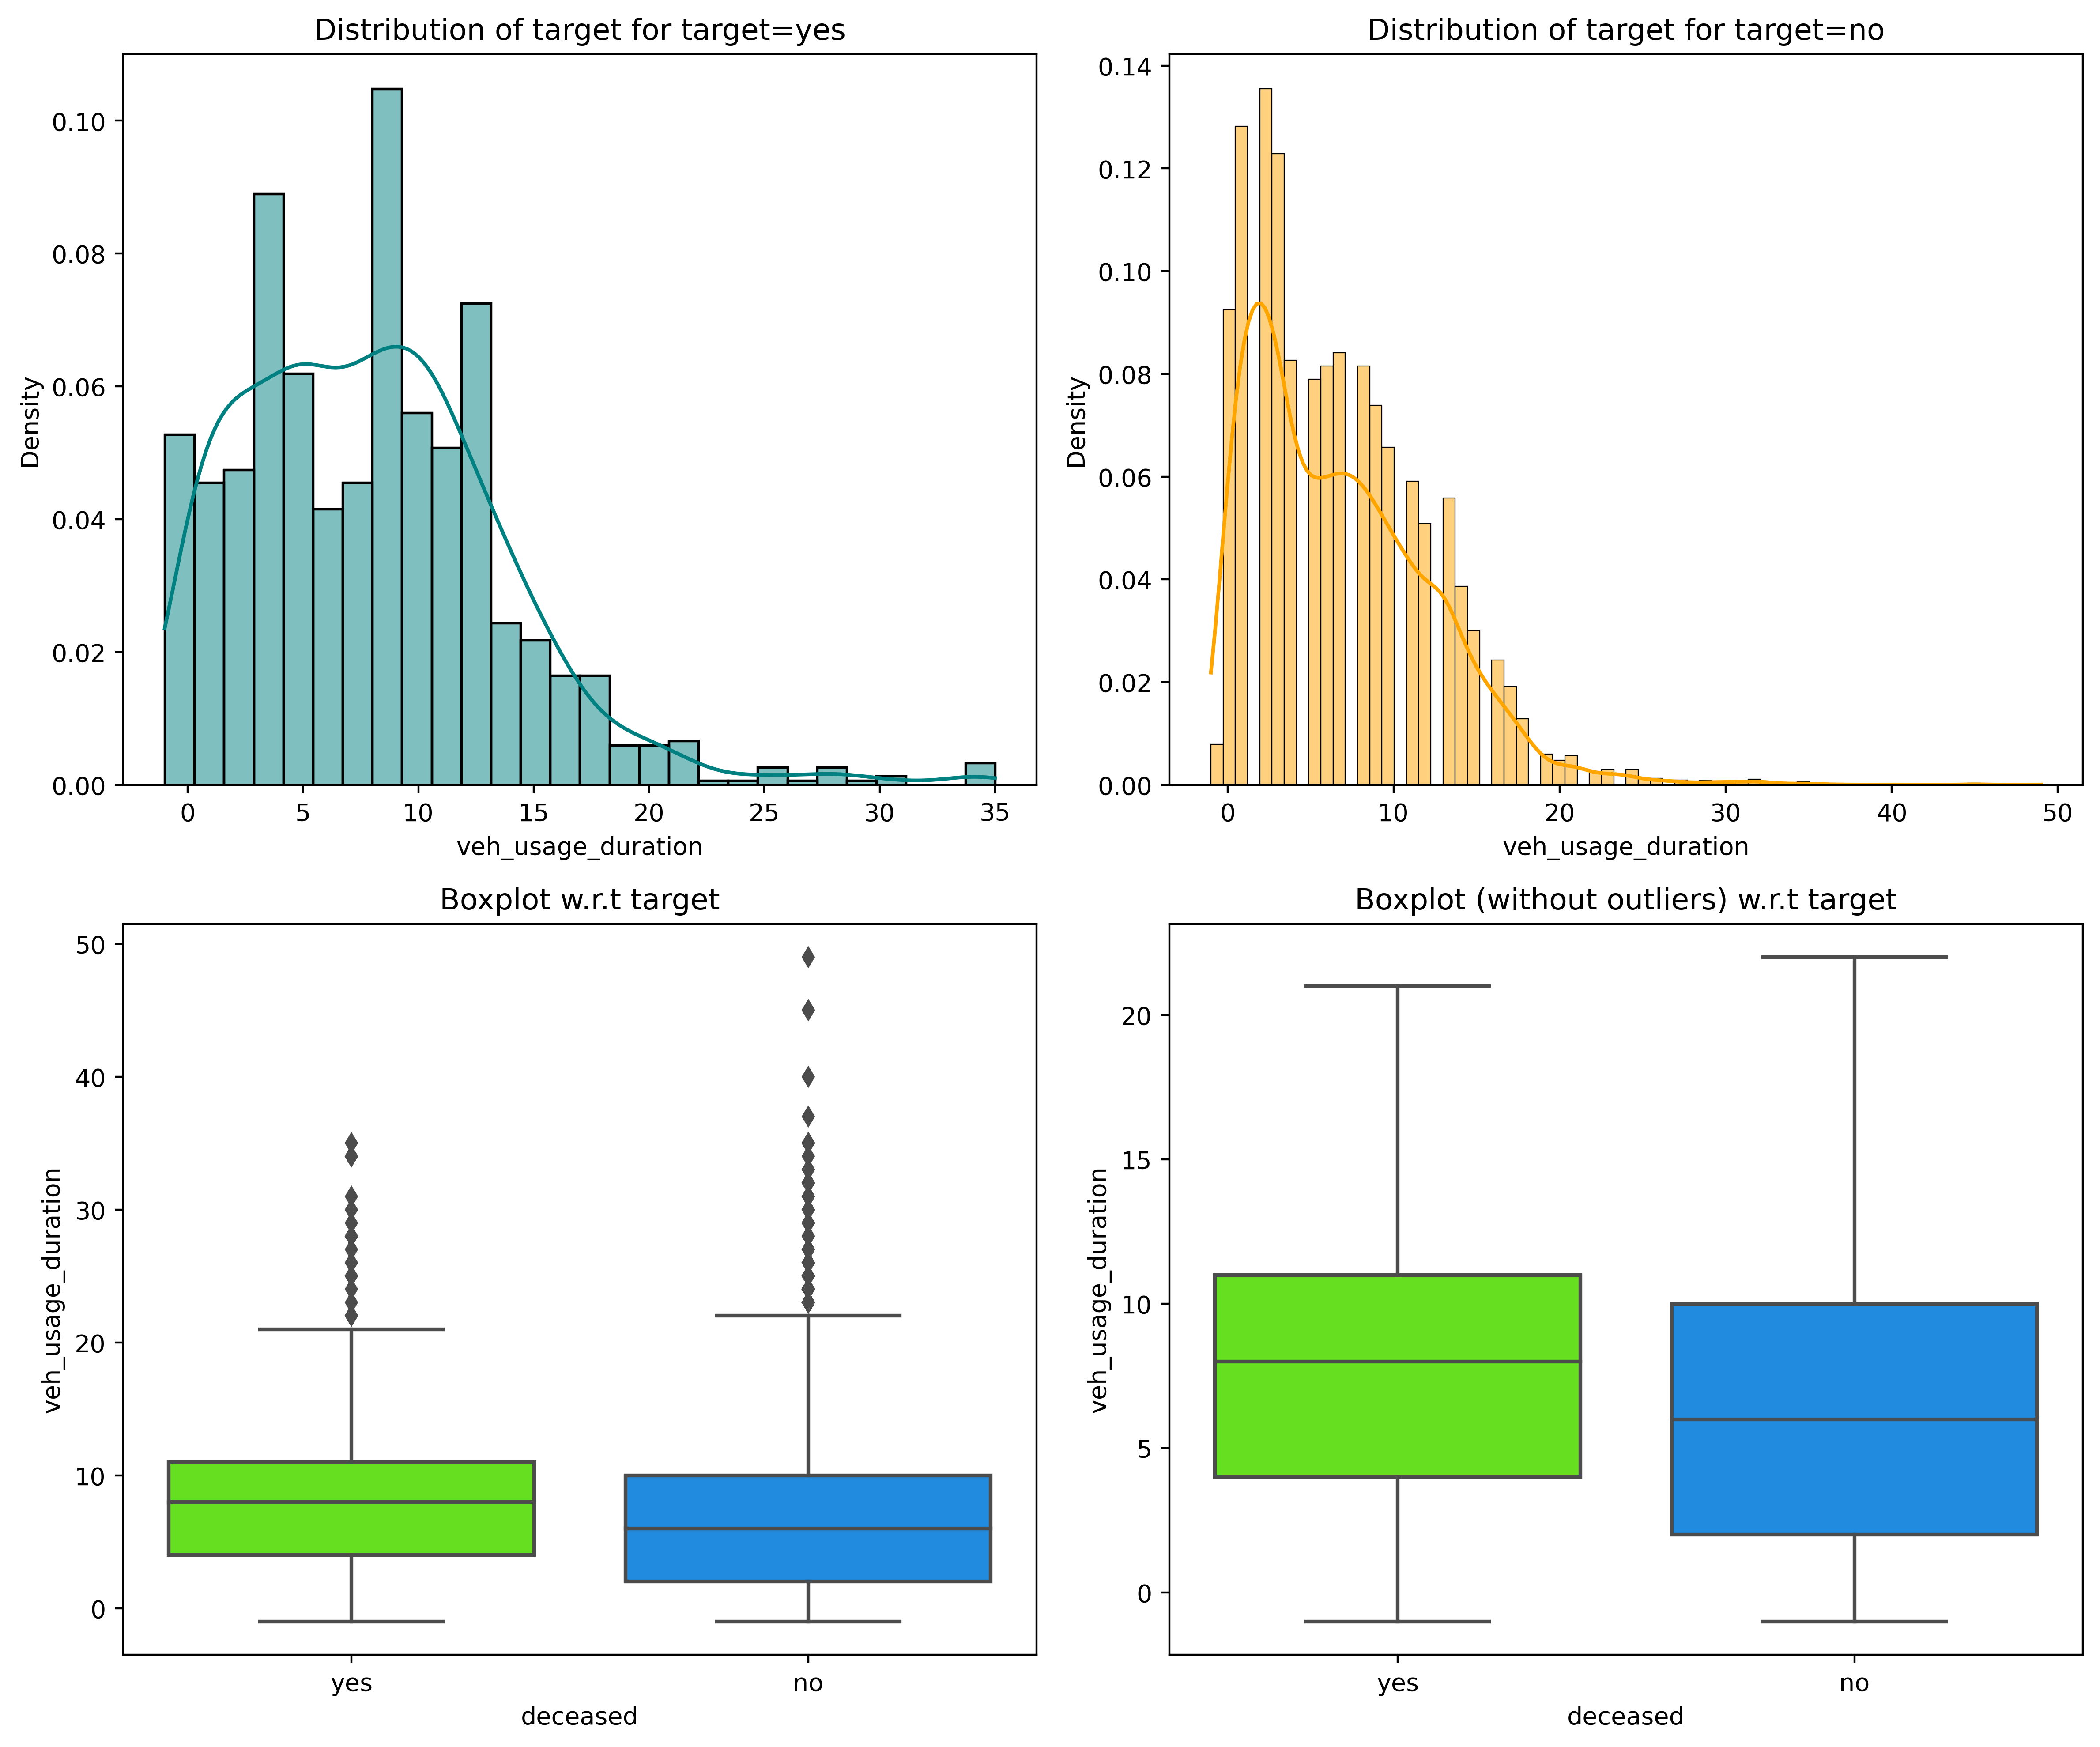
\includegraphics[width=\linewidth]{veh_usage_dur_wrt_target.png}
			\caption{Boxplot of deceased with respect to vehicle usage duration.}
			\label{fig:veh_usage_dur_wrt_target.png}
		\end{subfigure}
		\hfill
		\begin{subfigure}[t]{0.495\linewidth}
			\centering
			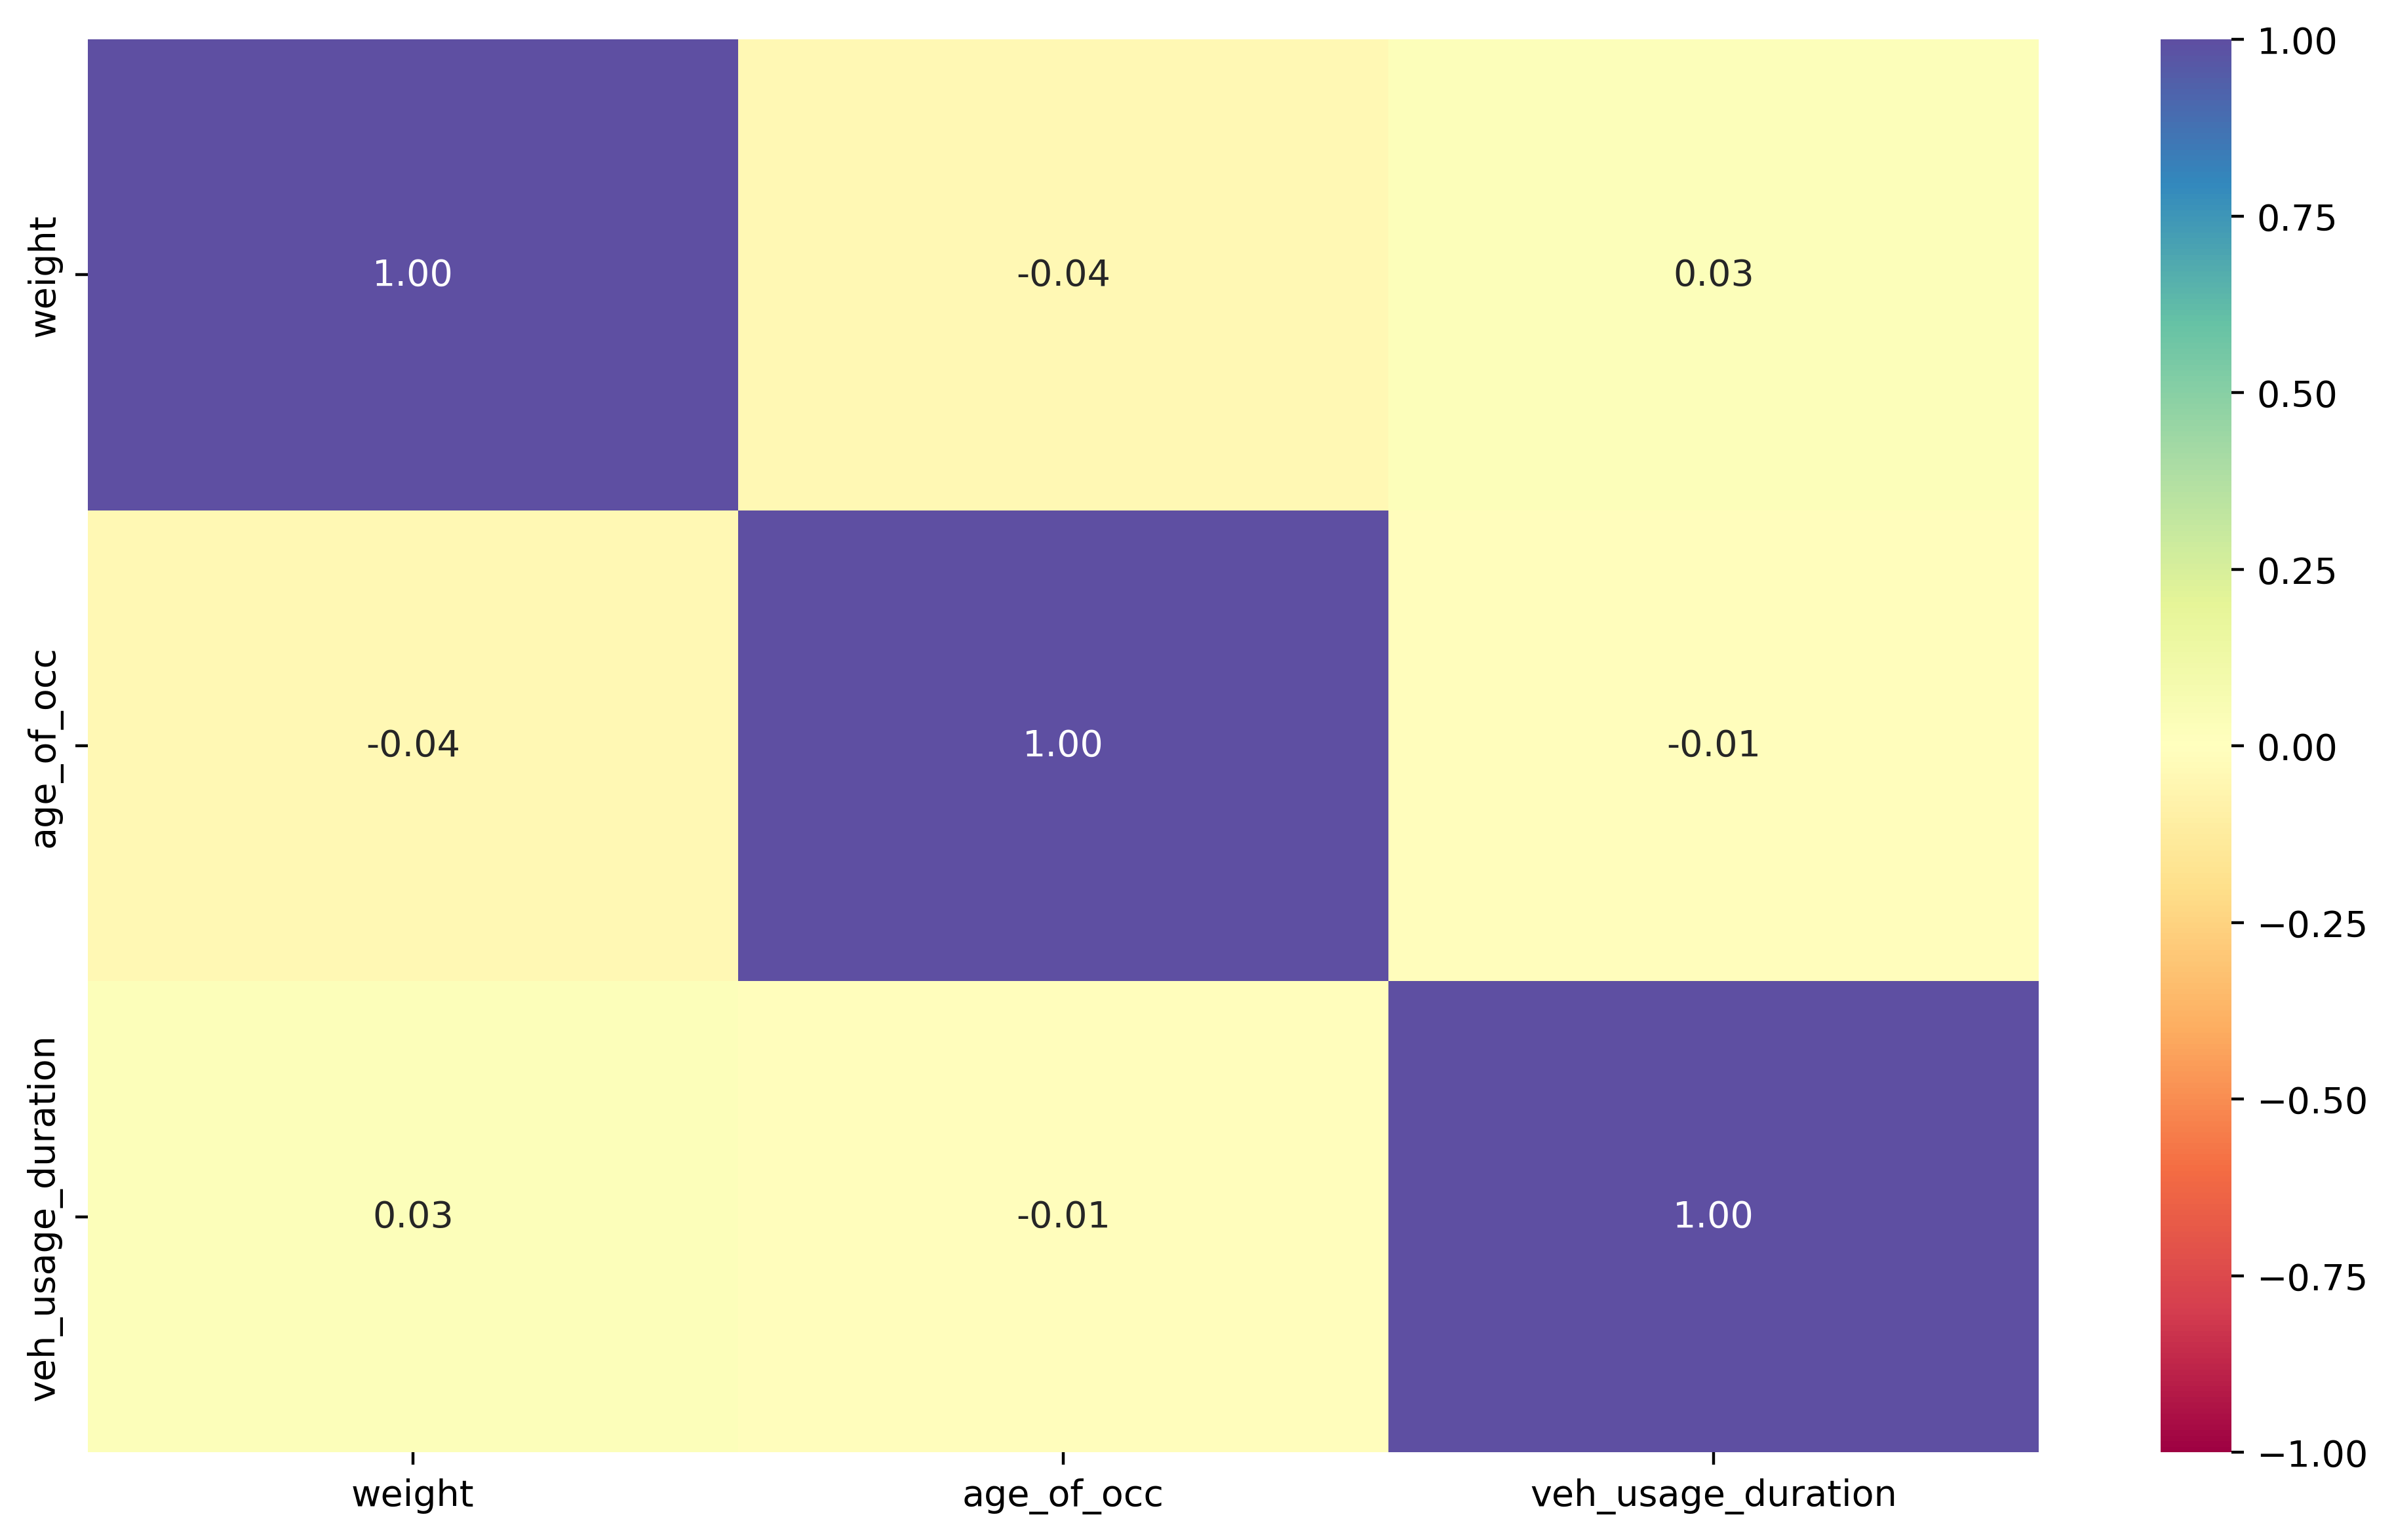
\includegraphics[width=\linewidth]{corr.png}
			\caption{Plot showing correlation among numerical variables.}
			\label{fig:corrt}
		\end{subfigure}
		\caption{}
		\label{fig:veh_usage_dur_wrt_target and corr }
	\end{figure}
	
The plot on figure \ref{fig:corrt} shows the correlation between numerical variables. The off-diagonal elements indicate very weak correlations between different variables. The variables weight, age\_of\_occ, and veh\_usage\_duration are largely independent of each other, as indicated by the near-zero correlation values.
	%%%%%%%%%%%%%%%%%%%%%%%%%%%%%%%%%%%%%%%%%%%%%%%%%%%%%%%%%%%%%%%%%%%%%%%%%
	\section{DataPreprocessing}
	Outliers are data points within a dataset that deviate significantly from the majority—they are either much larger or much smaller than the other values. We have checked the outliers present in the given data set using the boxplots. The dataset contains several outliers. Since these are genuine values, we have decided not to remove or adjust them, and will keep them as they are. 
	
	Feature scaling is a crucial data preprocessing technique that standardizes the values of features or variables within a dataset, ensuring they are on a similar scale. This process prevents larger values from disproportionately influencing the model. It's particularly important in datasets with features that vary widely in range, as such variation can lead to biased performance or learning difficulties.
	
	We can achieve this by using the StandardScaler, which standardizes the data so that the mean of each feature becomes zero and the standard deviation becomes one. After applying the StandardScaler, all features will be on the same scale, allowing us to proceed with model building.
	
	\begin{figure}[h]
		\centering
		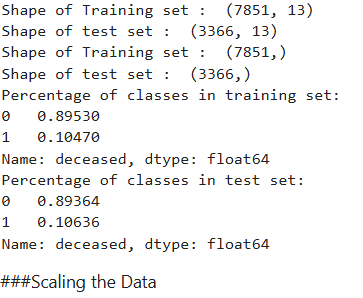
\includegraphics[width=0.5\textwidth]{train_test_split.png}
		\caption{Train and Test data set split}
		\label{fig:dataset_split}
	\end{figure}
	
	\section{Analysis with ML Models}
	In this section we have implemented following ML models to address the classification problem in our data set : Logistic regression, KNN, Naive Bayes and Decision Trees. But before we describe the implemented models, we should reflect on our motivation behind how we evaluate these models pertaining to the business problem at our hand. We want to predict the defaulters/deceased cases with as much efficiently as possible because catching these vulnerable cases will save lives. We observed that only 10 \% of the data set has deceased or defaulter. So even if we predict all the data set as non-defaulter/negatives, then also we would get 90 \% accuracy. Hence total model accuracy is not a good measure of model performance. Instead we should focus on Recall - It gives the ratio of True positives to Actual positives, so high Recall implies low false negatives, i.e. low chances of predicting a defaulter as non defaulter. That is what we have followed to tune our models and maximize the Recall.   
	\subsection{Logistic Regression}
	Logistic regression is a fundamental statistical method used in machine learning for binary classification tasks. It models the probability that a given input belongs to a particular class. Unlike linear regression, which predicts continuous outcomes, logistic regression predicts discrete outcomes by applying a logistic function to the linear combination of input features. This function, also known as the sigmoid function, maps predicted values to probabilities between 0 and 1.
	More precisely we carry out a linear model for the log of odds of the event y=1 and features X. Suppose probability of y=1 is $f_{w,b}$ , then the model is :
	\begin{equation}
		\log{\left(\frac{f_{w,b}}{1-f_{w,b}}\right)} = w_1\times x_1 + .... + w_k\times x_2 + b = \boldsymbol{W.X} + b
	\end{equation} 
	From this coefficients  we can compute the probabilities as (which comes out s the sigmoid function):
	\begin{equation}
		f_{w,b}(X)=\frac{1}{1+\exp{(w.X+b)}}
	\end{equation}
	The coefficients are computed by the optimization of log liklihood($L_{w,b}$) estimation/probability. So the cost function is :
	\begin{equation}
		\log{(L_{w,b})} = \log(\Pi_j P(y=y_j|X, w, b)) = \sum_{j=1}^{N}\left[ y_j\times \log(f_{w,b}(X)) + (1-y_j)\times \log(1-f_{w,b}(X))  \right] 
	\end{equation}
	\begin{figure}[h]
		\centering
		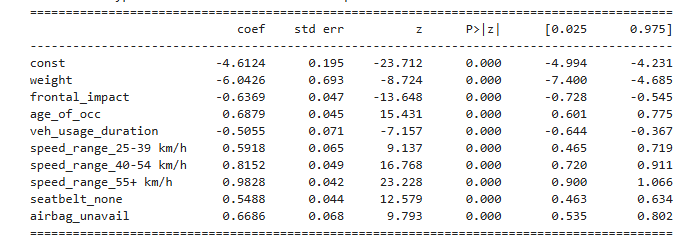
\includegraphics[width=0.8\linewidth]{lg2_summary.png}
		\caption{Logistic regression model building summary}
		\label{fig:lg2_summary}
	\end{figure}
	We have used logistic regression from statsmodel library in python. 
	\begin{figure}[h]
		\centering
		\begin{subfigure}[t]{0.49\textwidth}
			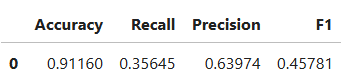
\includegraphics[width=\textwidth]{lg_base_train_perf.png}
			\caption{Performance on training set.}
			\label{fig:lg_base_train_perf}
		\end{subfigure}
		\hfill
		\begin{subfigure}[t]{0.49\textwidth}
			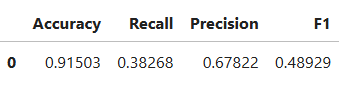
\includegraphics[width=\textwidth]{lg_base_test_perf.png}
			\caption{Performance on test set.}
			\label{fig:lg_base_test_per}
		\end{subfigure}
		\begin{subfigure}[t]{0.5\textwidth}
			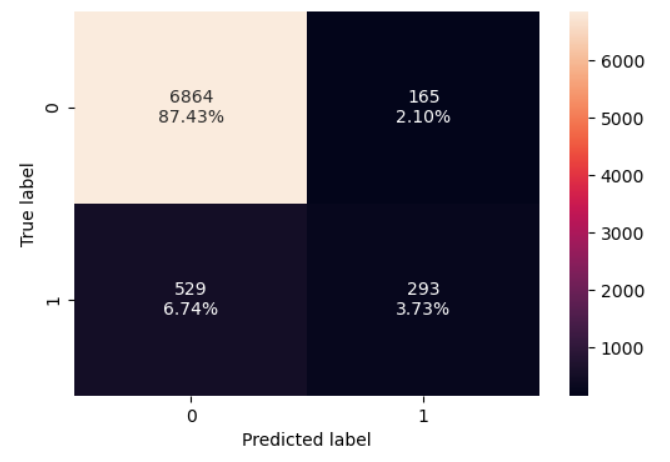
\includegraphics[width=\textwidth]{lg_base_c_Matrix_train.png}
			\caption{Confusion matrix on training set.}
			\label{fig:lg_base_c_Matrix_train}
		\end{subfigure}
		\hfill
		\begin{subfigure}[t]{0.45\textwidth}
			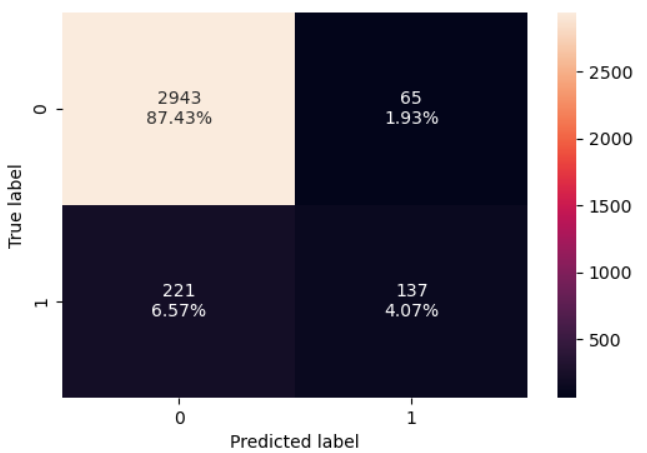
\includegraphics[width=\textwidth]{lg_base_c_Matrix_test.png}
			\caption{Confusion matrix on test set.}
			\label{fig: lg_base_c_Matrix_test}
		\end{subfigure}
		\caption{Model performance of Base logistic regression model.}
		\label{fig:Model performance of Base logistic regression model}
	\end{figure}
	
	After removing features with high p values, the result summary is shown in figure \ref{fig:lg2_summary}. After this we determined the optimal threshold using ROC Curve. The optimal threshold was found to be 0.11. Using this tuned model the model performance is shown in the figure \ref{fig:Model performance of tuned logistic regression model}. In the training data set we got a Recall of 86.13 \% and in test data 85.47 \%. Since the performnaces are similar in both training and testing we can conclude that there is no over fitting in the model. Using this tuned model we can predict the defaulters with 85.47 \% of recall which is much better than the base model which only had 38\% recall.  
	\begin{figure}[h]
		\centering
		\includegraphics[width=0.5\linewidth]{roc_auc.png}
		\caption{ROC AUC curve}
		\label{fig:roc_auc}
	\end{figure}
	%%%%%%%%%%%%%%%%%%%%%%%%%%%%%


	\begin{figure}[h]
		\centering
		\begin{subfigure}[t]{0.49\textwidth}
			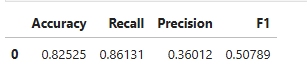
\includegraphics[width=\textwidth]{lg2_train_perf.png}
			\caption{Performance on training set.}
			\label{fig:lg2_train_perf}
		\end{subfigure}
		\hfill
		\begin{subfigure}[t]{0.49\textwidth}
			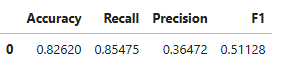
\includegraphics[width=\textwidth]{lg2_test_perf.png}
			\caption{Performance on test set.}
			\label{fig:lg2_test_per}
		\end{subfigure}
		\begin{subfigure}[t]{0.5\textwidth}
			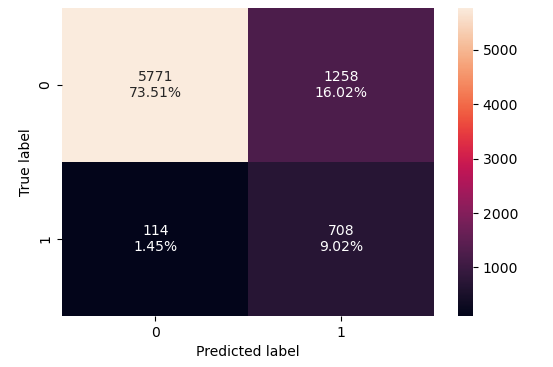
\includegraphics[width=\textwidth]{lg2_c_Matrix_train.png}
			\caption{Confusion matrix on training set.}
			\label{fig:lg2_c_Matrix_train}
		\end{subfigure}
		\hfill
		\begin{subfigure}[t]{0.45\textwidth}
			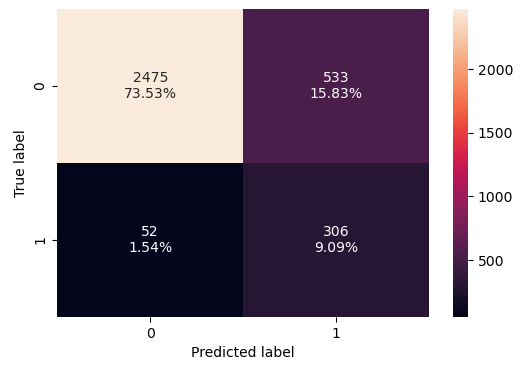
\includegraphics[width=\textwidth]{lg2_c_Matrix_test.png}
			\caption{Confusion matrix on test set.}
			\label{fig: lg2_c_Matrix_test}
		\end{subfigure}
		\caption{Model performance of tuned logistic regression model.}
		\label{fig:Model performance of tuned logistic regression model}
	\end{figure}
	\clearpage
	%%%%%%%%%%%%%%%%%%%%%%%%%%%%
	\subsection{K-Nearest Neighbor}
	The k-nearest neighbors (k-NN) algorithm is a simple yet powerful non-parametric method used for both classification and regression tasks in machine learning. It operates on the principle of proximity, where the classification or prediction for a given data point is determined by the ‘k’ closest training examples in the feature space.
	%%%%%%%%%%%%%%%%%%%%%%%%%%%%%
	\begin{figure}[h]
		\centering
		\begin{subfigure}[t]{0.49\textwidth}
			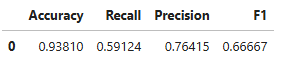
\includegraphics[width=\textwidth]{knn3_train_perf.png}
			\caption{Performance on training set.}
			\label{fig:knn3_train_perf}
		\end{subfigure}
		\hfill
		\begin{subfigure}[t]{0.49\textwidth}
			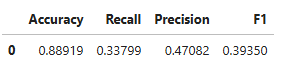
\includegraphics[width=\textwidth]{knn3_test_perf.png}
			\caption{performance on test set.}
			\label{fig:knn3_test_perf}
		\end{subfigure}
		\begin{subfigure}[t]{0.5\textwidth}
			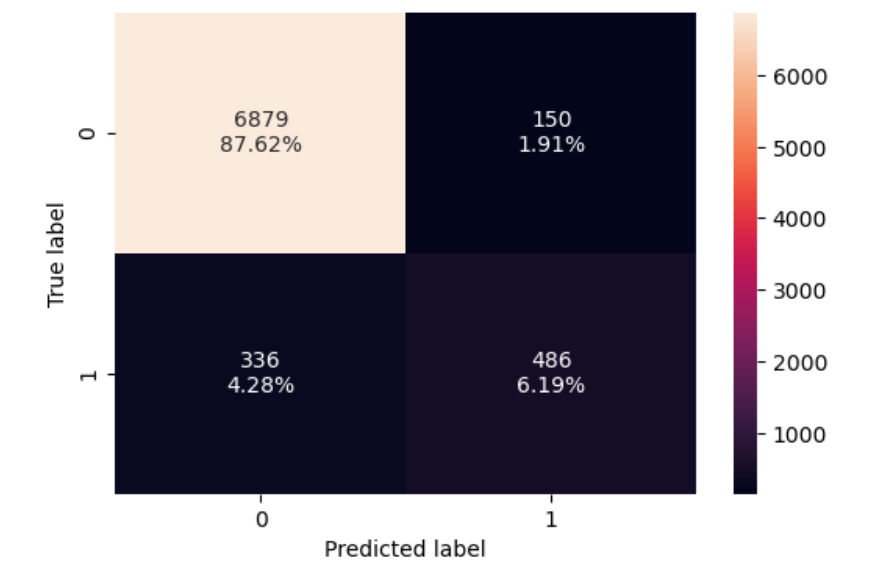
\includegraphics[width=\textwidth]{Knn3_c_Matrix_train.png}
			\caption{Confusion matrix on training set.}
			\label{fig:Knn3_c_Matrix_train}
		\end{subfigure}
		\hfill
		\begin{subfigure}[t]{0.45\textwidth}
			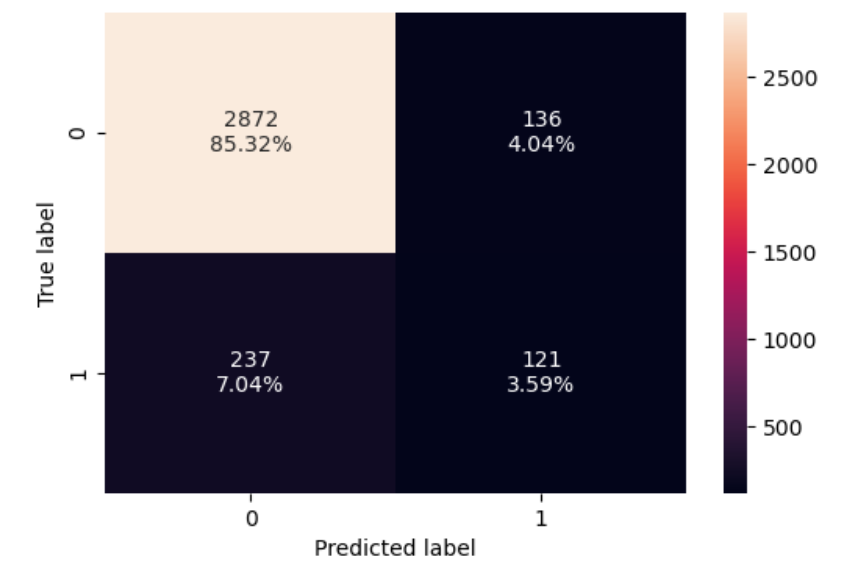
\includegraphics[width=\textwidth]{Knn3_c_Matrix_test.png}
			\caption{Confusion matrix on test set.}
			\label{fig: Knn3_c_Matrix_test}
		\end{subfigure}
		\caption{Model performance of KNN model. K=3.}
		\label{fig: Distribution of nmerical variables }
	\end{figure}	
	The optimum value of k=3 was found by recording the recall score for values of k from 2 to 20. Even though accuracy is quite good, knn model fails to provide us desired performance in terms of recall score. 
	%%%%%%%%%%%%%%%%	
	\subsection{Naive Bayes}
	The Naive Bayes classifier is a simple machine learning algorithm used for classification tasks. It is based on Bayes’ Theorem, which describes the probability of an event based on prior knowledge of conditions related to the event. The “naive” aspect of the algorithm comes from its assumption that all features are independent of each other given the class label, which is rarely true in real-world scenarios but simplifies the computation significantly. We carried out the Naive Bayes model from sklearn library. Similar to knn model, Naive Bayes model, although good with accuracy gives poor performance in terms of recall score. The performance on training and test data set is shown in figure \ref{fig:Model performance Naive Bayes Classifier.}
	%%%%%%%
	\begin{figure}[h]
		\centering
		\begin{subfigure}[t]{0.49\textwidth}
			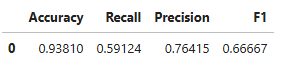
\includegraphics[width=\textwidth]{nb_train_perf.png}
			\caption{}
			\label{fig:nb_train_perf}
		\end{subfigure}
		\hfill
		\begin{subfigure}[t]{0.49\textwidth}
			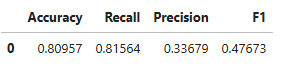
\includegraphics[width=\textwidth]{nb_test_perf.png}
			\caption{}
			\label{fig:nb_test_perf}
		\end{subfigure}
		\begin{subfigure}[t]{0.5\textwidth}
			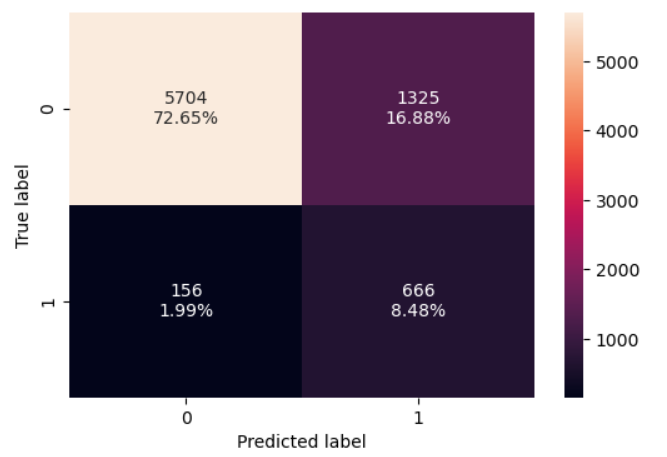
\includegraphics[width=\textwidth]{nb_c_Matrix_train.png}
			\caption{Confusion matrix on training set.}
			\label{fig:nb_c_Matrix_train}
		\end{subfigure}
		\hfill
		\begin{subfigure}[t]{0.45\textwidth}
			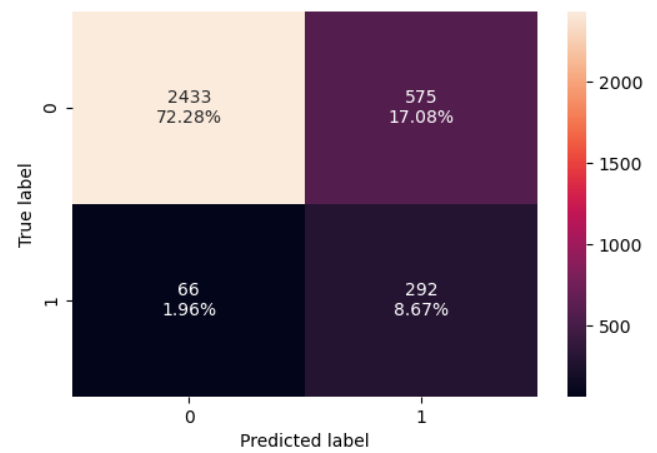
\includegraphics[width=\textwidth]{nb_c_Matrix_test.png}
			\caption{Confusion matrix on test set.}
			\label{fig: nb_c_Matrix_test}
		\end{subfigure}
		\caption{Model performance Naive Bayes Classifier.}
		\label{fig:Model performance Naive Bayes Classifier.}
	\end{figure}	
	%%%%%%
	\clearpage
	\subsection{Decision Trees}
	Decision tree classification is a powerful and intuitive machine learning technique used for both classification and regression tasks. It works by recursively splitting the dataset into subsets based on the value of input features, creating a tree-like model of decisions. Each internal node represents a decision point based on a feature, each branch represents the outcome of that decision, and each leaf node represents a class label or a continuous value. The algorithm uses criteria such as Gini impurity, entropy, or information gain to determine the best splits, aiming to create the most homogeneous branches possible. Decision trees are highly interpretable, as the resulting model can be visualized and easily understood, making them particularly useful for explaining predictions.
	We utilized pre-pruning techniques to enhance the performance of the Decision Tree model. Pre-pruning halted the growth of the decision tree at an earlier stage, preventing the model from becoming overly complex and reducing overfitting. This approach helped the model to generalize better and make more accurate predictions on unseen data.
	\begin{figure}[h]
		\centering
		\begin{subfigure}[t]{0.49\textwidth}
			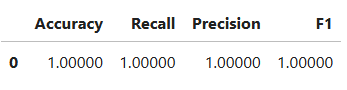
\includegraphics[width=\textwidth]{dTree_base_train_perf.png}
			\caption{}
			\label{fig:dTree_base_train_perf}
		\end{subfigure}
		\hfill
		\begin{subfigure}[t]{0.49\textwidth}
			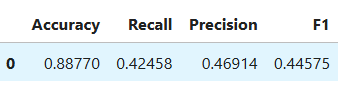
\includegraphics[width=\textwidth]{dTree_base_test_perf.png}
			\caption{}
			\label{fig:Tree_base_test_per}
		\end{subfigure}
		\begin{subfigure}[t]{0.47\textwidth}
			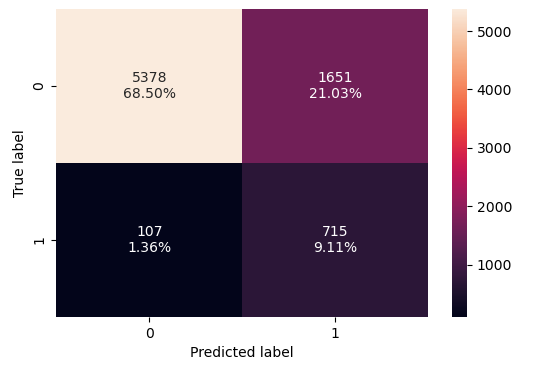
\includegraphics[width=\textwidth]{dTree_c_Matrix_train.png}
			\caption{}
			\label{fig:dTree_base_c_Matrix_trai}
		\end{subfigure}
		\hfill
		\begin{subfigure}[t]{0.45\textwidth}
			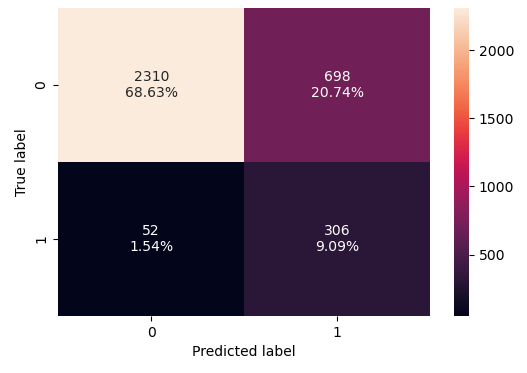
\includegraphics[width=\textwidth]{dTree_c_Matrix_test.png}
			\caption{}
			\label{fig:dTree_base_c_Matrix_test}
		\end{subfigure}
		\caption{Model Performance of Base Decision Tree grown to full length.}
		\label{fig:Model Performance of Base Decision Tree}
	\end{figure}
	
	To further refine the model, we applied hyperparameter tuning using GridSearchCV. This involved systematically searching through a predefined grid of hyperparameter values and evaluating each combination through cross-validation. By doing so, we aimed to find the optimal parameters that maximize the performance metric, thus improving the model’s generalization and effectiveness. We explored various parameter combinations for the DecisionTreeClassifier from sklearn, including max depth, min samples split, max leaf nodes, and class weight. The goal was to identify the best configuration that delivers superior performance for our dataset.
	
	After conducting the GridSearchCV process, the ideal set of parameters for the DecisionTreeClassifier was determined as follows:
	\begin{figure}[h]
		\centering
		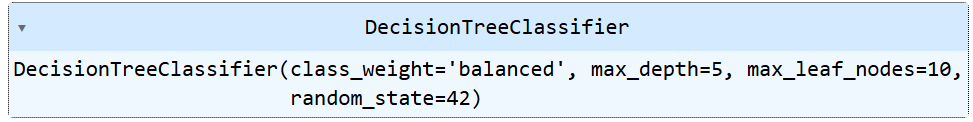
\includegraphics[width=0.8\linewidth]{Tuned_dtree_classifier}
		\caption{Decision Tree classifier obtained from GridSearchCV (Pre-pruning).}
		\label{fig:Tuned_dtree_classifiers}
	\end{figure}
	
	%%%%%%%%%%%%%%%%%%%%%%%%%%%%%
	\begin{figure}[h]
		\centering
		\begin{subfigure}[t]{0.49\textwidth}
			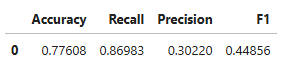
\includegraphics[width=\textwidth]{dTree_train_perf.png}
			\caption{}
			\label{fig:dTree_train_perf}
		\end{subfigure}
		\hfill
		\begin{subfigure}[t]{0.49\textwidth}
			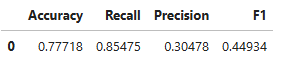
\includegraphics[width=\textwidth]{dTree_test_perf.png}
			\caption{}
			\label{fig:Tree_test_per}
		\end{subfigure}
		\begin{subfigure}[t]{0.47\textwidth}
			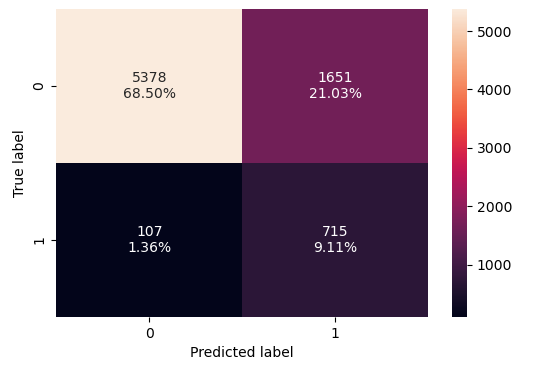
\includegraphics[width=\textwidth]{dTree_c_Matrix_train.png}
			\caption{}
			\label{fig:dTree_c_Matrix_trai}
		\end{subfigure}
		\hfill
		\begin{subfigure}[t]{0.45\textwidth}
			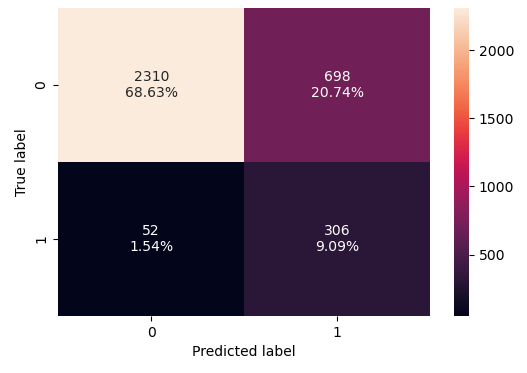
\includegraphics[width=\textwidth]{dTree_c_Matrix_test.png}
			\caption{}
			\label{fig:dTree_c_Matrix_test}
		\end{subfigure}
		\caption{Model Performance of Tuned Decision Tree (Pre-pruning).}
		\label{fig:Model Performance of Decision Tree}
	\end{figure}
	\begin{figure}[h]
	\centering
	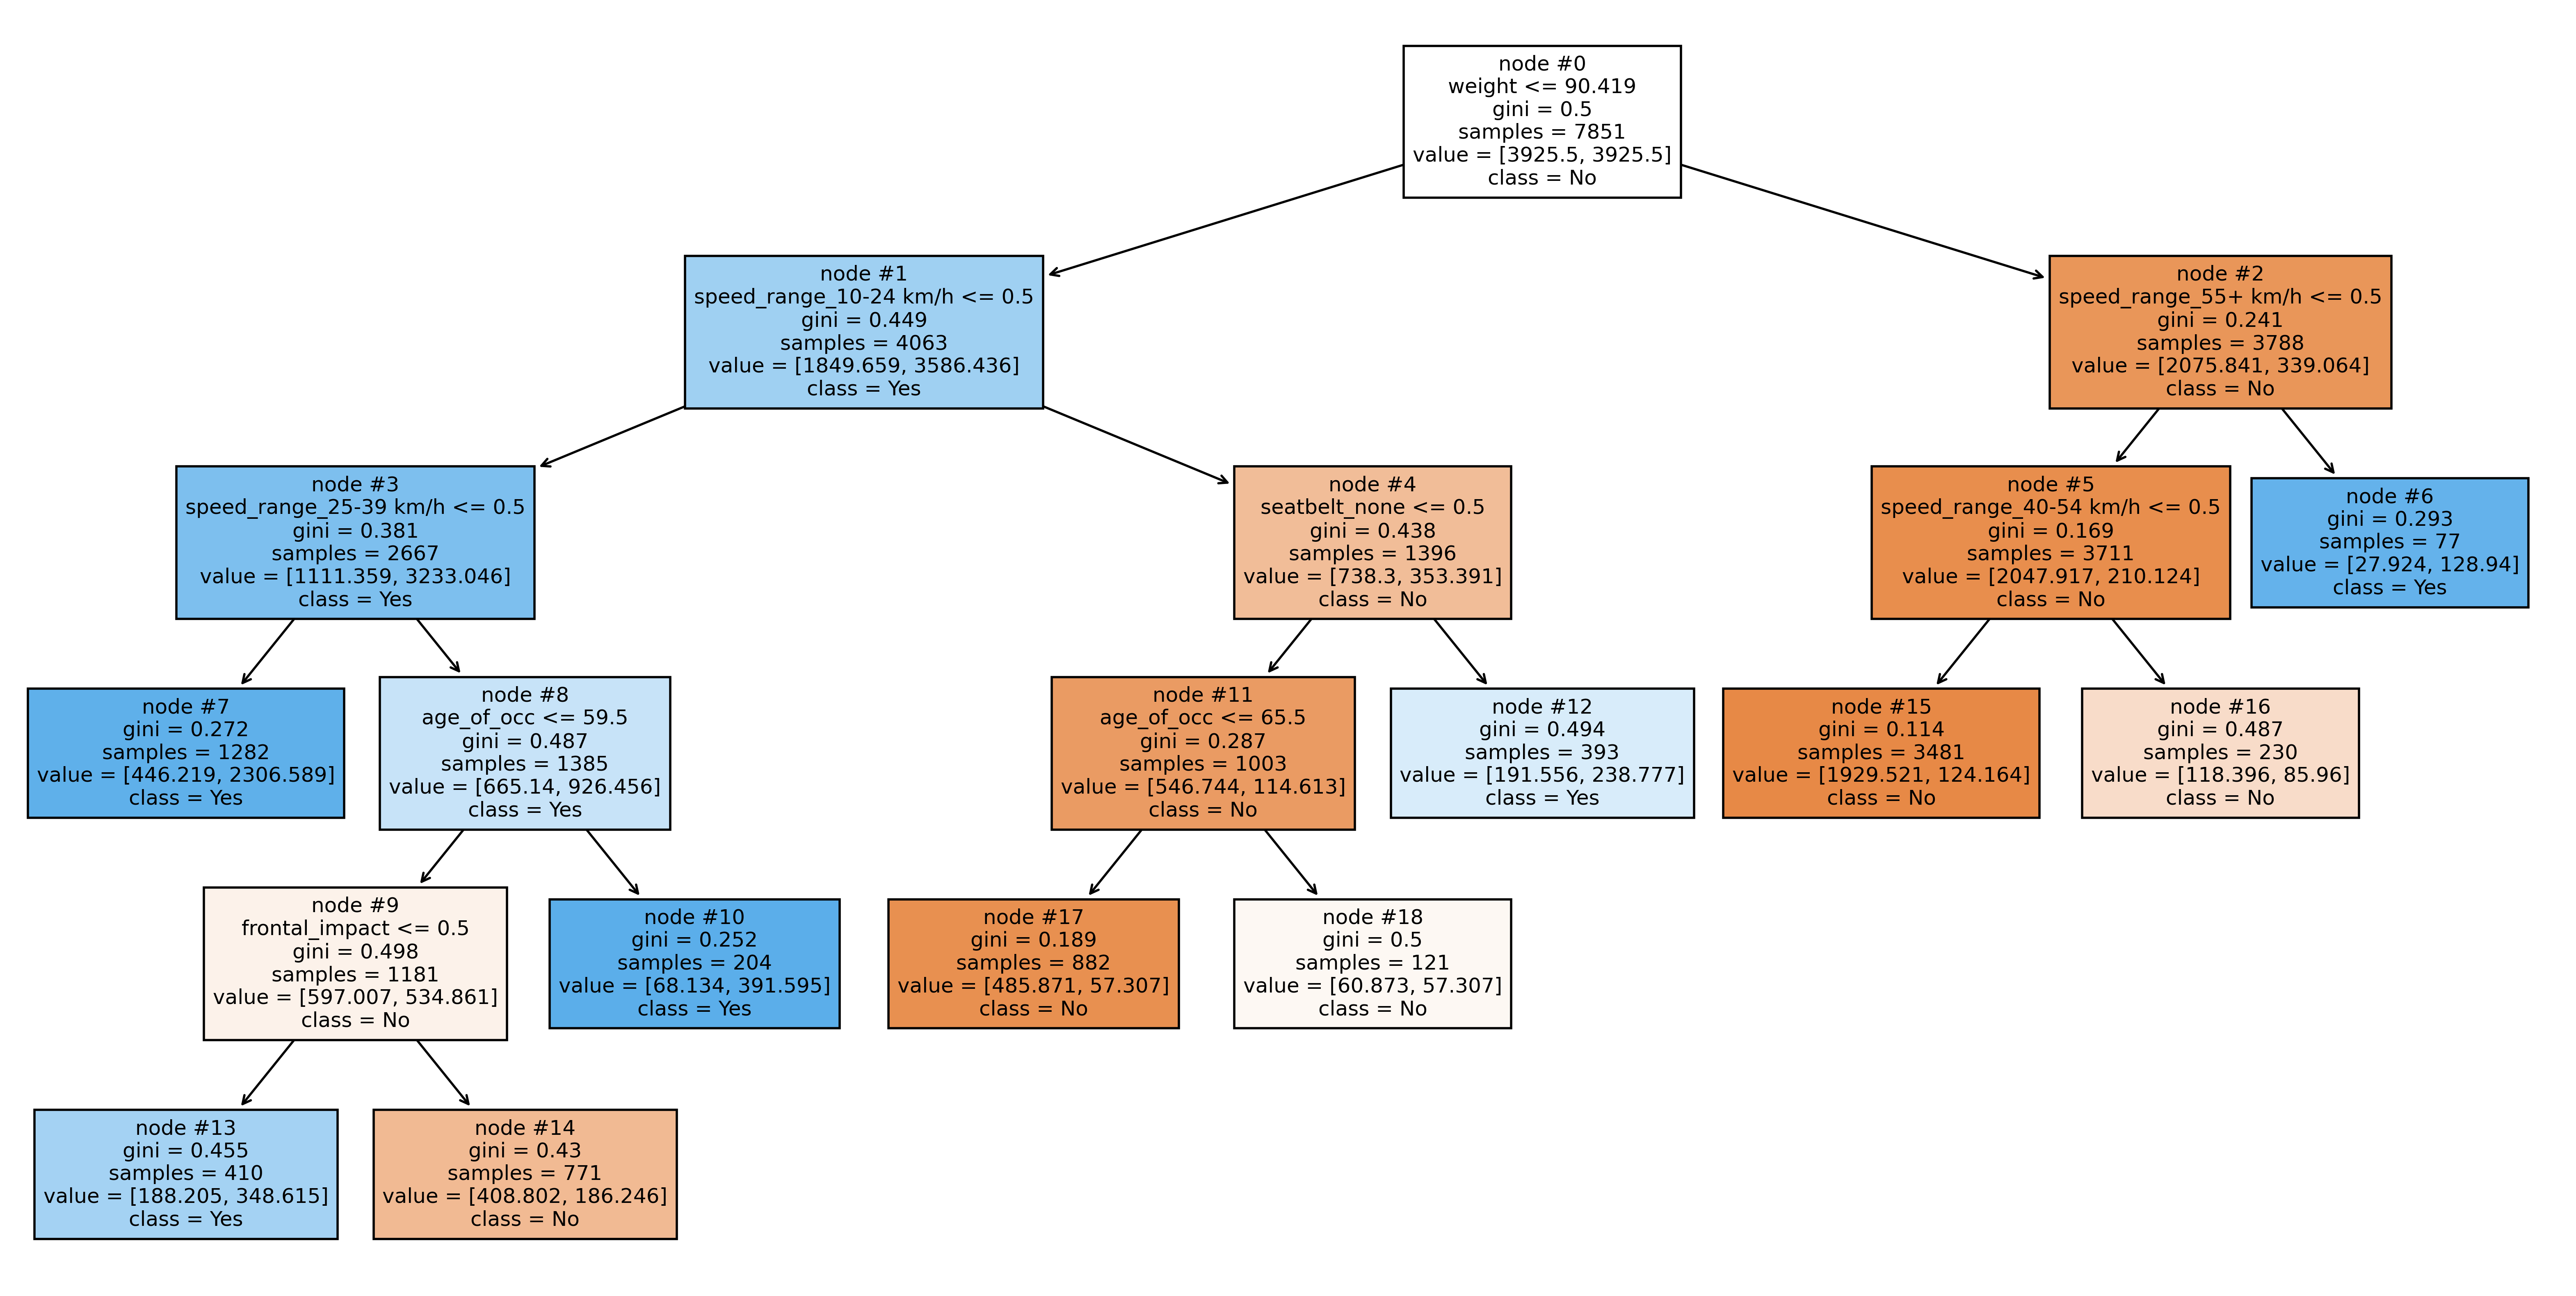
\includegraphics[width=0.7\linewidth]{dTree_vis.png}
	\caption{Decision Tree visualization of the tuned model. (Pre-pruning)}
	\label{fig:dTree_vis}
	\end{figure}
	
	\begin{figure}[h]
		\centering
		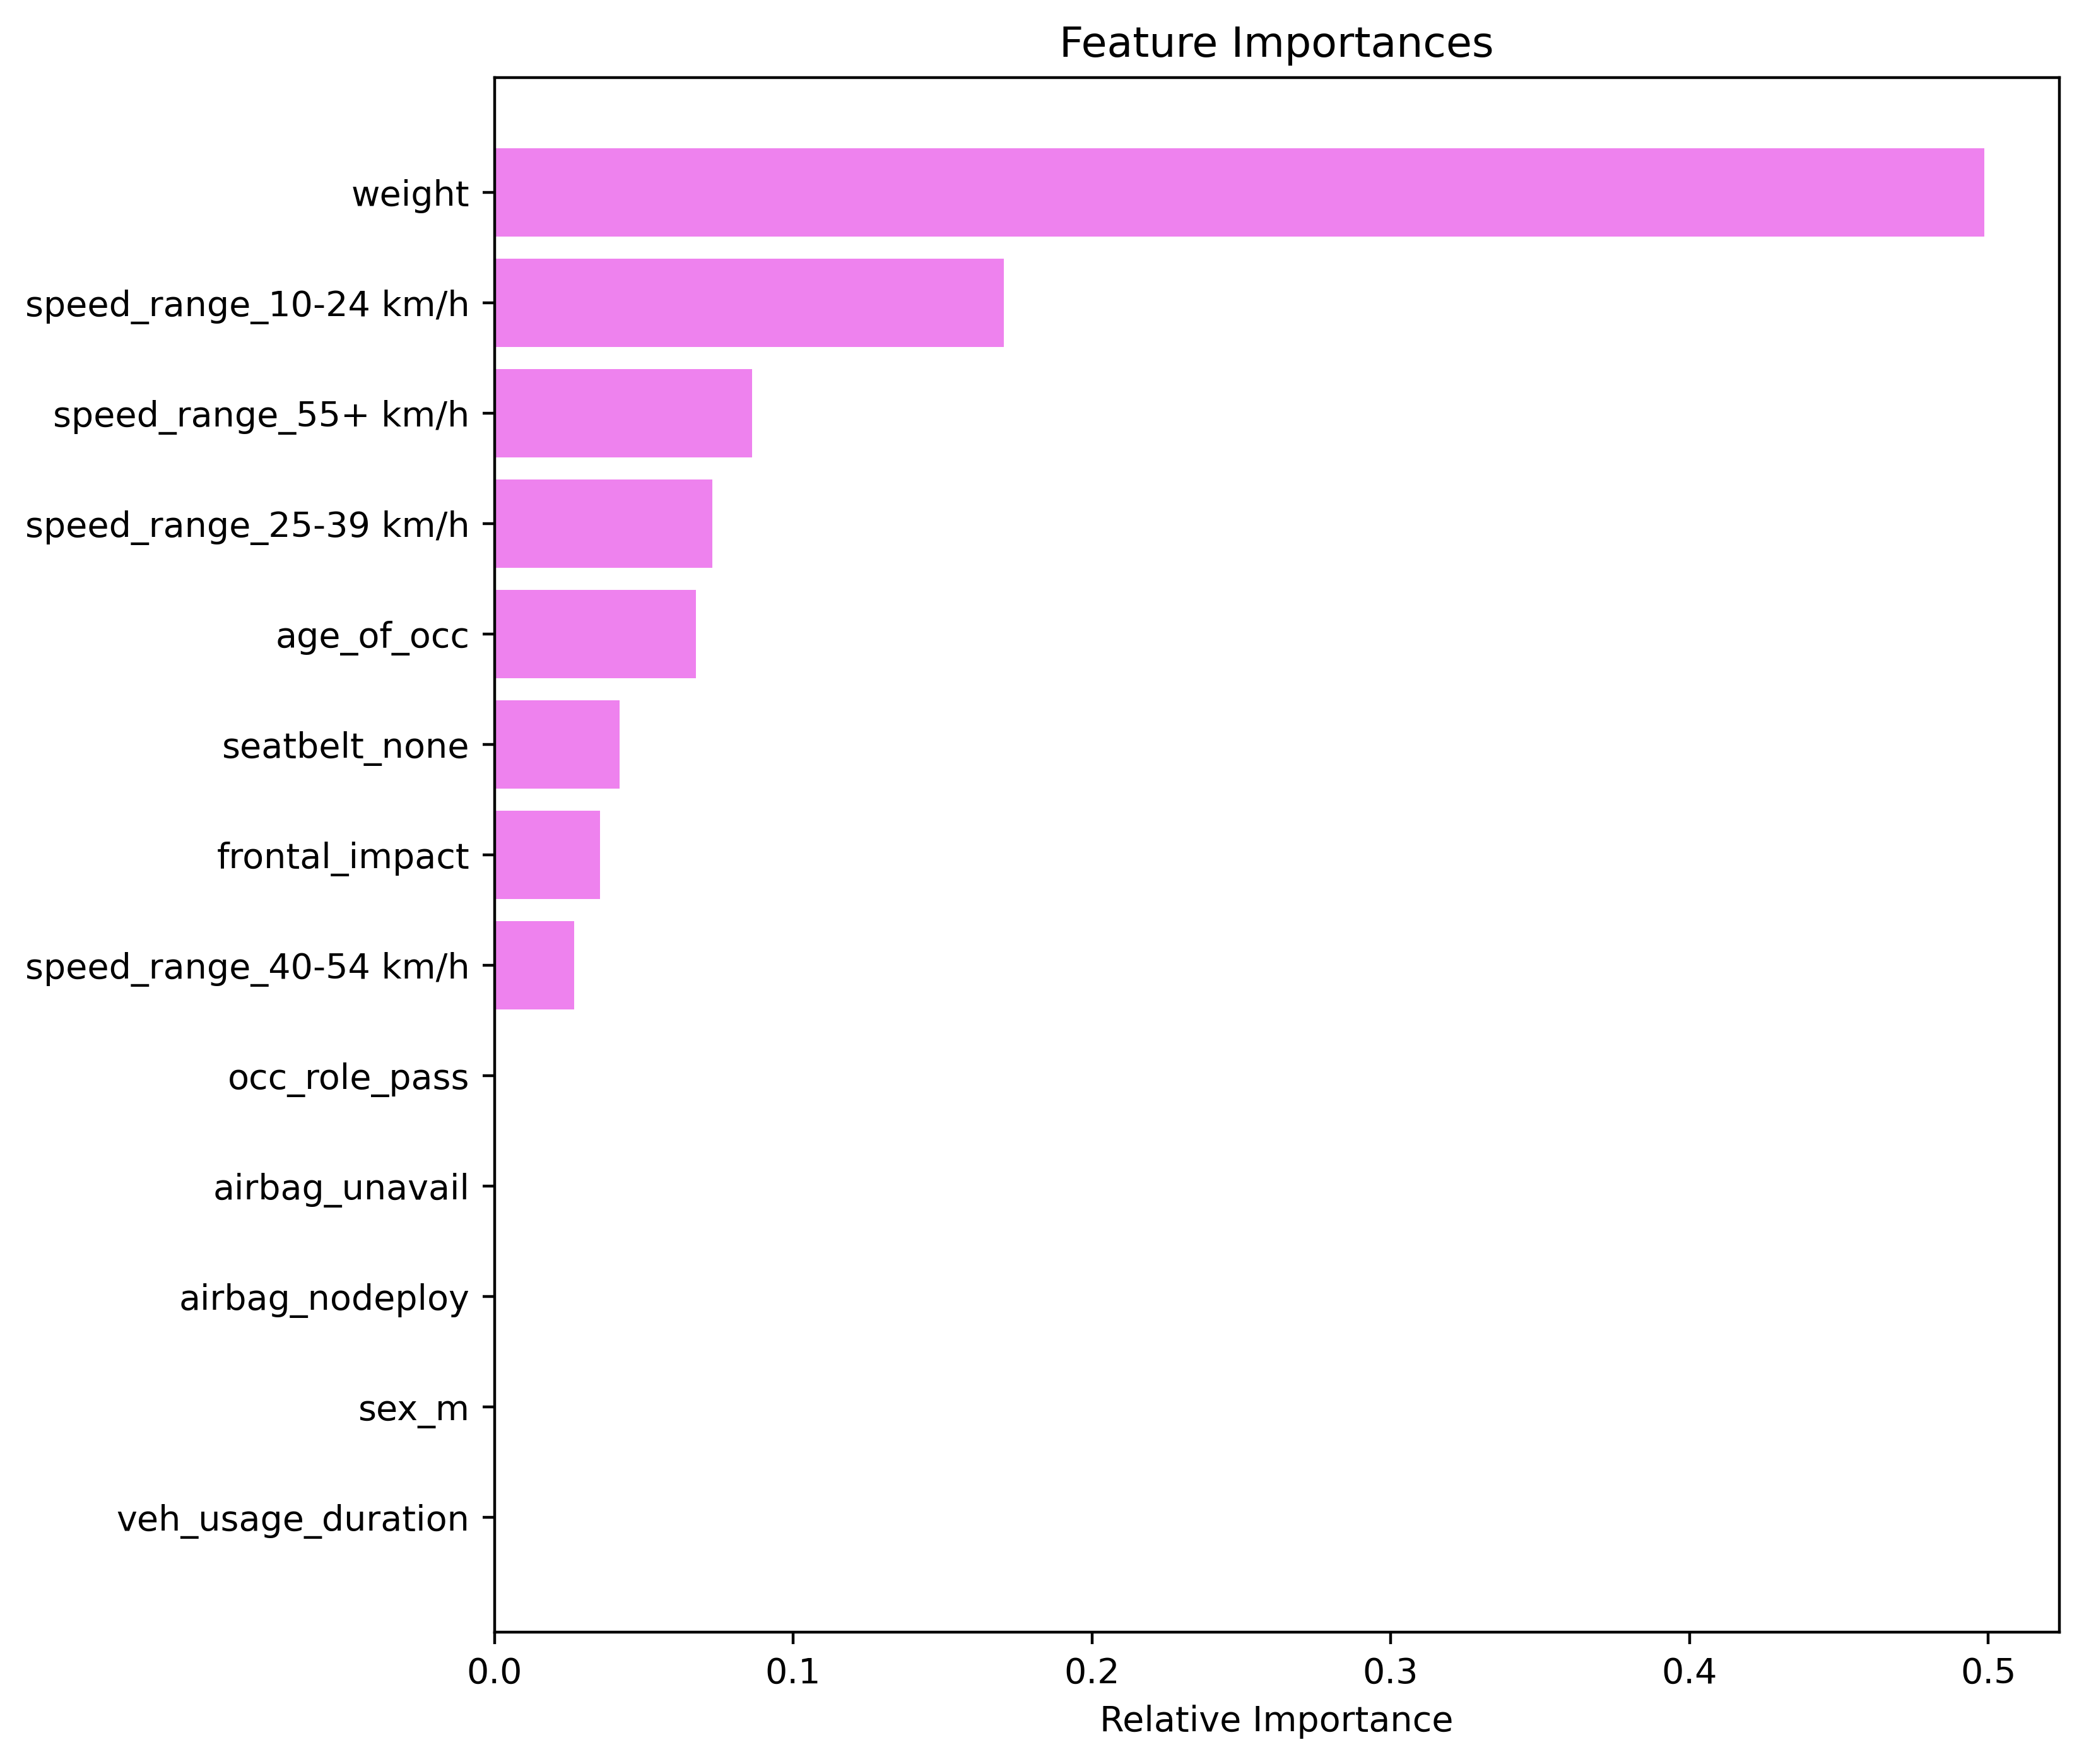
\includegraphics[width=\linewidth,height=9cm]{_feat_importance.png}
		\caption{Importance of features as inferred from tuned decision tree model (pre-pruning)}
		\label{fig:feat_imp}
	\end{figure}
	The visualization for the tuned decision tree is shown in figure \ref{fig:dTree_vis}. It has a depth of 6. The feature importance is obtained from this tuned model which is shown in figure \ref{fig:feat_imp}. Weight, speed of vehicle, age, configuration of seat belt and whether there was a frontal impact are most features in deciding survival chances from crash. Having a speed range of 55+ km/h generally associated more with mortality as we had observed during EDA. The weight of the vehicle involved in the accident which turns out to be most important factor has more mortality rate for accident when < 90.5 as observed from the top node of decision tree. So, lighter vehicles are more prone to damages and fatal crashes and associated with higher mortality rate. This is also confirmed from the box plot with respect to weight. Similarly higher age associated more with mortality.
	%%%%%%%%%%%%%%%%%%%%%%%%%%%%	
	\clearpage
	\subsection{Final Model comparison}
	\begin{figure}[h]
		\centering
		\includegraphics[width=\linewidth]{training_perf_compare.png}
		\caption{Comparison of base and tuned model performance on training set.}
		\label{fig:training_perf_copmpare}
	\end{figure}

	\begin{figure}[h]
		\centering
		\includegraphics[width=\linewidth]{test_perf_copmpare.png}
		\caption{Comparison of base and tuned model performance on test set.}
		\label{fig:test_perf_copmpare}
	\end{figure}
	
	\begin{itemize}
		\item Logistic regression accuracy is quite good both on training and testing data set. This signifies good level of generalization. After tuning to find the optimal threshold it show good performance on recall as well.
		\item Naive bayes and KNN on the otherhand although perform good interms of accuracy in both training and testing, they failed to deliver good performance in terms of recall score.
		\item Complete Base decision tree severely over fits the training data giving perfect accuracy. But this over fitting is exposed in the performance on testing set which is significantly lower.  
		\item Pre prunned decision tree performs much better with similar score on training and test data set. This shows good level of generalization. The recall score 0f 85.5 \% is achieved in test set through grid search and cross validation.
	\end{itemize}
	
	%%%%%%%%%%%%%%%%%%%%%%%%%%%%%%%%%%%%%%%%%%%%%%%%%%%%%%%%%%%%%%%%%%%%%%%%%%
	\section{Actionable insights and Recommendations}
	\subsection{Actionable insights}
	\begin{itemize}
	\item The analysis reveals that vehicle weight is the most significant factor in determining survival chances in crashes. Lighter vehicles (weighing less than 90.5) are associated with a higher mortality rate. This insight suggests that enhancing the structural integrity of lighter vehicles could potentially reduce fatalities.
	\item Vehicles traveling at speeds greater than 55 km/h are more likely to be involved in fatal crashes. Implementing stricter speed regulations and promoting safe driving practices at high speeds can significantly enhance survival rates in accidents.
	\item Higher age is correlated with an increased mortality rate in crashes. This underscores the importance of targeted safety measures for older adults, such as advanced driver assistance systems and age-specific vehicle safety features.
	
	\item The configuration of seat belts and the occurrence of frontal impacts are critical factors influencing survival chances. Encouraging the use of proper seat belt configurations and enhancing frontal impact safety features in vehicles can improve overall crash survivability.
	
	\item The analysis shows a slight difference in fatalities between males and females, with males having slightly more fatalities. This could be attributed to factors such as driving behavior or exposure risk, suggesting the need for targeted safety interventions based on gender-specific risk factors.
	
	\item The distribution of fatalities based on the occupant's role reveals that passengers are more prone to severe outcomes compared to drivers. This is likely due to the lack of high-efficiency airbags in passenger seats. Enhancing safety features for all occupants, including passengers, can reduce the vulnerability in crashes.
	
	
		
	\end{itemize}
	
	\subsection{Business Recommendations}
	\begin{itemize}
	\item Focus on innovative materials and structural design improvements for lighter vehicles. Private companies should be encouraged to Allocate a significant portion of the R and D budget to develop stronger, more resilient materials that can enhance the safety of lighter vehicles without significantly increasing their weight. Educate consumers about the enhanced safety features and structural improvements in lighter vehicles.
	
	\item Advocate for and implement stricter speed limits, especially in high-risk areas where crashes are more frequent. Collaborate with local authorities and law enforcement to ensure compliance and promote safe driving practices. Use technology such as speed cameras and dynamic speed signs to monitor and manage vehicle speeds effectively.  Launch awareness campaigns and educational programs that highlight the risks associated with driving at speeds greater than 55 km/h. Provide resources and training for drivers to adopt safer driving habits, focusing on speed management and defensive driving techniques.
	
	\item Develop and implement advanced driver assistance systems (ADAS) tailored to the needs of older drivers. These could include features like lane departure warnings, automatic emergency braking, and adaptive cruise control. Additionally, design and promote vehicle safety features that cater specifically to older adults, such as adjustable seat belts and ergonomic controls.
	
	\item Establish a system for continuous monitoring of crash data and effectiveness of speed regulations and safety measures. Use this data to make informed decisions and implement necessary improvements.
	
	\item Launch comprehensive awareness campaigns focusing on the importance of using seat belts properly. Provide clear instructions and demonstrations on the correct seat belt usage. Collaborate with automotive manufacturers to include reminders and alerts for proper seat belt configurations in vehicles.
	
	\end{itemize}
	\begin{centering}
		\vspace{20pt}
		\subsection*{End of Report\\Submitted by : Haraprasad Dhal}
	\end{centering}
\end{document}